%%%%%%%%%%%%%%%%%%%%%%%%%%%%%%%%%%%%
%
%                                MAIN OF MY BOOK
%                                 edupuis@cnam.fr
%
%%%%%%%%%%%%%%%%%%%%%%%%%%%%%%%%%%%%

%----------------------------------------------------------------------------------------
%	PACKAGES AND OTHER DOCUMENT CONFIGURATIONS
%----------------------------------------------------------------------------------------

%\documentclass[20pt,fleqn,twoside,openright]{book} % Default font size and left-justified equations

\documentclass[11pt,fleqn, a4paper,twoside,openright]{book}


%-------------------------------------------------------------
%               FR CYBERDEF SECOPS COURSE
%                         BOOK CONFIG
%					        2020 eduf@ction
%-------------------------------------------------------------

\newcommand{\utitle}{SECOPS}
%\newcommand{\ubooktitleBefore}{Cyberdéfense d'Entreprise}
\newcommand{\ubooktitleBefore}{DRAFT - NON CORRIGE}
\newcommand{\ubooktitleMain}{Eléments de sécurité opérationnelle}
\newcommand{\ubooktitle}{Sécurité opérationnelle}
\newcommand{\uBookname}{Eléments de sécurité opérationnelle}
%\newcommand{\ubooktitleAfter}{SECOPS SEC101}
\newcommand{\ubooktitleAfter}{...en travaux...}
\renewcommand{\uCoursetheme}{
\includegraphics[width=0.04\paperwidth]{Tex/template.inc/Commons/CommonsPictures/shield-20.pdf} }

\renewcommand{\ecours}{e document \xspace} 

\renewcommand{\INFODistrib}{EN TRAVAUX NE PAS DIFFUSER}




%\PassOptionsToPackage{unicode}{hyperref}
%\PassOptionsToPackage{naturalnames}{hyperref}

\usepackage{beamerarticle}

\usepackage{ae}
\usepackage[french]{babel}
\usepackage[utf8]{inputenc}
\usepackage[T1]{fontenc}

\usepackage{ccicons}



\usepackage{titletoc} % Required for manipulating the table of contents

%===========================
% EDX PACKAGE
%===========================

\usepackage [hyphens]{url}

\usepackage[utf8]{inputenc}
\usepackage[french]{babel}
\usepackage[T1]{fontenc}



\usepackage{tikz} % Required for drawing custom shapes
\usetikzlibrary{tikzmark} 
\usetikzlibrary{mindmap,trees, backgrounds}
\usepackage{verbatim}
\usepackage{wrapfig}
\usepackage{xpatch}

\usepackage{hologo}

\usepackage{fontawesome}

\usepackage[skins]{tcolorbox} % don't forget SKINS option

\usepackage{listings}
\usepackage{upquote}

\lstset{
upquote=true,columns=flexible, basicstyle=\ttfamily,
language=HTML, 
frameround=tttt,
commentstyle=\color{gray},
identifierstyle=\color{blue},
keywordstyle=\color{ocre}\bfseries,
xleftmargin=2em,
xrightmargin=2em,
aboveskip=\topsep,
belowskip=\topsep, 
frame=single,
rulecolor=\color{ocre},
backgroundcolor=\color{ocre!5},
breaklines,
breakindent=1.5em,
showspaces=false,
showstringspaces=false,
showtabs=false,
}


\usepackage{graphicx} % Required for including pictures
\graphicspath{{Pictures/}} % Specifies the directory where pictures are stored

\usepackage{booktabs} % Required for nicer horizontal rules in tables

\usepackage{setspace}
\setstretch{1,1}

\usepackage{csquotes}

\usepackage{fancyhdr}

\usepackage{makeidx} 

\usepackage{xspace} 

\usepackage{titletoc} % Required for manipulating the table of contents

\usepackage[breaklinks, pdftex]{hyperref}

\hypersetup{pdftitle={\utitle},pdfauthor={\uauthor},hidelinks,backref=true,pagebackref=true,hyperindex=true,colorlinks=false,breaklinks=true,urlcolor=ocre,bookmarks=true,bookmarksopen=false}

%\pdfstringdefDisableCommands{%
%  \def\\{}%
%  \def\texttt#1{<#1>}%
%}

\usepackage[style=numeric,citestyle=numeric,sorting=nyt,sortcites=true,autopunct=true,babel=hyphen,hyperref=true,abbreviate=false,backref=true,backend=biber]{biblatex}

\usepackage{cleveref}



%===========================
% EDX COMMAND STANDART
%===========================

\newcommand\UKword[1]{\emph{#1}}
\newcommand\Ucenter[1]{\begin{center}{#1}\end{center}}

\newcommand\head[1]{\textbf{#1}}
\newcommand\tb[1]{\textbf{#1}}
\newcommand{\g}[1]{\og #1 \fg{}}
\newcommand{\uload}[1] {\input{../Tex/#1}}
\newcommand{\ucurcolor}{black}

\newcommand{\mak}[1]{\faicon{\aArrowCircleORight} #1}
%-----------------------------------------------------
%										 	\upspicture 
%---------------------------------------------------
\newcommand{\upspicture}[3]
{
\renewcommand{\ucurcolor}{#3}
\resizebox{#2\textwidth}{!}{\input{#1}}
}

%-----------------------------------------------------
%										 	\uchap
%---------------------------------------------------
\ifdefined\INTERTITLE
\newcommand{\uchap}[1]
	{
	\begin{LARGE}
	\textbf{\Ucenter{#1 \\ -oOo-}}	
	\end{LARGE}
	}
\else
	\newcommand{\uchap}[1]{}
\fi

%-----------------------------------------------------
%											\uexpand
%---------------------------------------------------
\newcommand {\uexpand}[1]{
\mode<all>\input{../Tex/Chapters/#1}
}

%-----------------------------------------------------
%											\upicture 
%---------------------------------------------------

\newcommand{\upicture}[4]{
\begin{figure}[!h] %h
  \begin{center}
	 \includegraphics[width=#3\textwidth]{#1.pdf}
  \end{center}
\caption{#2 \label{#4}}
\end{figure}
}


%-----------------------------------------------------
%											\uref 
%---------------------------------------------------
\newcommand{\uref}[1]{(Voir~\cref{#1} page~\pageref{#1})}



%-----------------------------------------------------
%											\updfimage 
%---------------------------------------------------

\newcommand{\updfimage}[3]
{
\begin{wrapfigure}{R}{#3\textwidth}
  \begin{center}
	 \resizebox{#3\textwidth}{!}{\includegraphics{#1.pdf}}
  \end{center}
\caption{#2}
\end{wrapfigure}
}



%************************PACKAGE***

%\usepackage{tikz}% Required for drawing custom shapes
\usetikzlibrary{shadows}


%-----------------------------------------------------
%											 		\rem 
% insertion d'une remarque avec R
%---------------------------------------------------
\newcommand\rem[1]{%
   \marginpar{%
   \tikzpicture[baseline={(title.base)}]
      \node[inner sep=5pt,text width=4cm,drop shadow={shadow yshift=-5pt,shadow xshift=5pt,ocre},fill=white] (box) {\vskip5pt \nointerlineskip #1};
      \node[right=10pt,inner sep=0pt,outer sep=10pt] (title) at (box.north west) {\bfseries\color{ocre}Remarque};
      \draw[draw=ocre,very thick](title.west)--(box.north west)--(box.south west)--(box.south east)--(box.north east)--(title.east);
      \fill[ocre]([yshift=-10pt]box.north west)--+(-5pt,-5pt)--+(0pt,-10pt);
   \endtikzpicture}%
}
%-----------------------------------------------------
%											 \utikzimage 
% insertion d'une image sur fichier tkz.tex
%---------------------------------------------------

\newcommand{\utikzimage}[3]
{
\begin{wrapfigure}{R}{#3\textwidth}
  \begin{center}
	 \resizebox{#3\textwidth}{!}{\input{#1.tkz.tex}}
  \end{center}
\caption{#2}
\end{wrapfigure}
}

%-----------------------------------------------------
%														\link 
% Url et footnote du lien
%-----------------------------------------------------
  
%  \newcommand{\link}[2]
%  {
%  \href{#1}
%  {
%  #2~\raisebox{-0.2ex}{\footnote
%  	{
% #1
%  	}
%  }
%  }
%  }
  
  
    \newcommand{\link}[2]
  {
  \href{#1}
  {
  #2~\raisebox{-0.2ex}{\faExternalLink}\footnote
  	{
 #1
  	}
  }
  }
  

  %-----------------------------------------------------
%														\Pframe 
% Beamer Frame
%-----------------------------------------------------




%\newenvironment{Pframe}[1]{\mode<all>{\begin{frame}<presentation>\frametitle{#1}}{\end{frame}}}
%
%\newenvironment{Tframe}[1]{{\begin{frame}<presentation>\frametitle{#1}}{\end{frame}}
%
%
%\newenvironment{Aframe}{\begin{frame}}{\end{frame}}
%

%\newcommand{\Aframetitle}[1]
%{
%\mode<presentation>{\frametittle{#1}}
%}
%













%===========================
% EDX STYLE
%===========================

\usepackage{parskip}
\setlength{\parindent}{10pt}
\setlength{\parskip}{5pt} % 1ex plus 0.5ex minus 0.2ex}

%---------------------------------------------------------------
%	MARGINS
%---------------------------------------------------------------

\usepackage{geometry}

\geometry{
	paper=a4paper, 
	top=4cm, 
	bottom=4cm, 
	left=3cm, 
	right=3cm, 
	headheight=20pt, 
	footskip=1.4cm, 
	headsep=10pt, 
%	showframe, 
	showcrop 
}



\makeatletter
\long\def\@makefntextFB#1{%
    \ifx\thefootnote\ftnISsymbol
        \@makefntextORI{#1}%
    \else
        \rule\z@\footnotesep
        \setbox\@tempboxa\hbox{\@thefnmark}%
            \ifdim\wd\@tempboxa>\z@
                \kern2em\llap{\@thefnmark.\kern0.5em}%
            \fi
        \hangindent2em\hangafter\@ne#1
    \fi}
\makeatother

 %-----------------------------------------------------------------------
%	COLOR
%-----------------------------------------------------------------------

%\usepackage{xcolor} % Required for specifying colors by name
\definecolor{ocre}{RGB}{160,0,0}   
                 
%-----------------------------------------------------------------------
%	FONTS
%-----------------------------------------------------------------------

%%\usepackage{avant} % Use the Avantgarde font for headings
%\usepackage{times} % Use the Times font for headings
%\usepackage{mathptmx} % Use the Adobe Times Rgman as the default text font together with math symbols from the Sym­bol, Chancery and Com­puter Modern fonts

%%\usepackage{microtype} % Slightly tweak font spacing for aesthetics
%%\usepackage[utf8]{inputenc} % Required for including letters with accents
%\usepackage[T1]{fontenc} % Use 8-bit encoding that has 256 glyphs

% Using AVANT GARDE Family

%\renewcommand{\familydefault}{\sfdefault}

%\fontfamily{pag}\selectfont
%\renewcommand{\familydefault}{pag} % sfdefault pag lmss

%bch         Charter
%lmr         Latin Modern Roman
%lmss        Latin Modern Sans Serif
%lmssq       Latin Modern Sans Serif extended
%lmtt        Latin Modern Typewriter
%lmvtt       Latin Modern Typewriter proportional
%pag         Avant Garde
%pbk         Bookman
%pcr         Courier
%phv         Helvetica
%pnc         New Century Schoolbook
%ppl         Palatino
%ptm         Times
%put         Utopia



\renewcommand{\rmdefault}{pag} % text 
\renewcommand{\sfdefault}{phv} % titre


 %%\usepackage{fontspec}
 
		%\usepackage{unicode-math}
		%\defaultfontfeatures { Scale = 0.92  }
  
  
  
  %%\setmainfont{Fira Sans Light}
  
  
 		 %[Ligatures = TeX,Numbers = OldStyle]
 		 %\setmathfont{Lucida Bright}
 		 %\setmonofont{Lucida Bright}
  
  
  
 %% \setsansfont{Fira Sans}
 
 
  		%[ Extension = .otf, UprightFont = *-Book,ItalicFont = *-BookItalic,  BoldFont = *-SemiBold, BoldItalicFont = *-SemiBoldItalic,Scale = 0.95, Numbers = OldStyle ]
		%  \newfontfamily\fullcaps{Lucida Bright} [Extension = .otf,  UprightFont = *_DemiBold,Scale = 0.95,Numbers = Uppercase ]


%-------------------------------------------------------------------------
%	COLOR
%-------------------------------------------------------------------------

  %% Couleurs
 % \usepackage{xcolor}
  \definecolor{comments}{rgb}{0.7,0,0}    % rouge foncé
  \definecolor{link}{rgb}{0,0.4,0.6}      % ~RoyalBlue de dvips
  \definecolor{url}{rgb}{0.6,0,0}         % rouge-brun
  \definecolor{citation}{rgb}{0,0.5,0}    % vert foncé
  \definecolor{ULlinkcolor}{rgb}{0,0,0.3} % de ulthese.cls
  \definecolor{rouge}{rgb}{0.85,0,0.07}   % rouge bandeau identitaire
  \definecolor{or}{rgb}{1,0.8,0}          % or bandeau identitaire




%-------------------------------------------------------------------------
%	BIBLIOGRAPHY AND INDEX
%-------------------------------------------------------------------------

%usepackage[style=numeric,citestyle=numeric,sorting=nyt,sortcites=true,autopunct=true,babel=hyphen,hyperref=true,abbreviate=false,backref=true,backend=biber]{biblatex}
%\addbibresource{bibliography.bib} % BibTeX bibliography file
%\defbibheading{bibempty}{}

\usepackage{calc} % For simpler calculation - used for spacing the index letter headings correctly
\usepackage{makeidx} % Required to make an index
\makeindex % Tells LaTeX to create the files required for indexing

%-------------------------------------------------------------------------
%	HEADERS AND FOOTERS
%-------------------------------------------------------------------------

\usepackage{fancyhdr} % Required for header and footer configuration

\pagestyle{fancy} % Enable the custom headers and footers

\ifcsname chapter \endcsname   % verify if command name exists in the CLASS (Book, report, article ...)

\renewcommand{\chaptermark}[1]{\markboth{\sffamily\normalsize\bfseries\chaptername\ \thechapter.\ #1}{}} % Styling for the current chapter in the header
  \else
%nothing
\fi

\renewcommand{\sectionmark}[1]{\markright{\sffamily\normalsize\thesection\hspace{5pt}#1}{}} % Styling for the current section in the header

\fancyhf{} % Clear default headers and footers
\fancyhead[LE,RO]{\sffamily\normalsize\thepage} % Styling for the page number in the header
\fancyhead[LO]{\sffamily\normalsize\rightmark} % Print the nearest section name on the left side of odd pages
\fancyhead[RE]{\sffamily\normalsize\leftmark} % Print the current chapter name on the right side of even pages
\fancyfoot[RE,LO]{\sffamily\normalsize\ubooktitleMain} % Uncomment to include a footer
\fancyfoot[LE,RO]{\sffamily\normalsize\ubooksubtitle} % Uncomment to include a footer

\renewcommand{\headrulewidth}{1.0pt} % Thickness of the rule under the header

\fancypagestyle{plain}{% Style for when a plain pagestyle is specified
	\fancyhead{}\renewcommand{\headrulewidth}{0pt}%
}

% Removes the header from odd empty pages at the end of chapters
\makeatletter
\renewcommand{\cleardoublepage}{
\clearpage\ifodd\c@page\else
\hbox{}
\vspace*{\fill}
\thispagestyle{empty}
\newpage
\fi}

%----------------------------------------------------------------------------------------
%	MAIN TABLE OF CONTENTS
%----------------------------------------------------------------------------------------


%\usepackage{titletoc} % Required for manipulating the table of contents

\contentsmargin{0cm} % Removes the default margin

% Part text styling (this is mostly taken care of in the PART HEADINGS section of this file)
\titlecontents{part}
	[0cm] % Left indentation
	{\addvspace{20pt}\bfseries} % Spacing and font options for parts
	{}
	{}
	{}

% Chapter text styling
\titlecontents{chapter}
	[1.25cm] % Left indentation
	{\addvspace{12pt}\large\sffamily\bfseries} % Spacing and font options for chapters
	{\color{ocre!60}\contentslabel[\Large\thecontentslabel]{1.25cm}\color{ocre}} % Formatting of numbered sections of this type
	{\color{ocre}} % Formatting of numberless sections of this type
	{\color{ocre!60}\normalsize\;\titlerule*[.5pc]{.}\;\thecontentspage} % Formatting of the filler to the right of the heading and the page number

% Section text styling
\titlecontents{section}
	[1.25cm] % Left indentation
	{\addvspace{3pt}\sffamily\bfseries} % Spacing and font options for sections
	{\contentslabel[\thecontentslabel]{1.25cm}} % Formatting of numbered sections of this type
	{} % Formatting of numberless sections of this type
	{\hfill\color{black}\thecontentspage} % Formatting of the filler to the right of the heading and the page number

% Subsection text styling
\titlecontents{subsection}
	[1.25cm] % Left indentation
	{\addvspace{1pt}\sffamily\small} % Spacing and font options for subsections
	{\contentslabel[\thecontentslabel]{1.25cm}} % Formatting of numbered sections of this type
	{} % Formatting of numberless sections of this type
	{\ \titlerule*[.5pc]{.}\;\thecontentspage} % Formatting of the filler to the right of the heading and the page number

% Figure text styling
\titlecontents{figure}
	[1.25cm] % Left indentation
	{\addvspace{1pt}\sffamily\small} % Spacing and font options for figures
	{\thecontentslabel\hspace*{1em}} % Formatting of numbered sections of this type
	{} % Formatting of numberless sections of this type
	{\ \titlerule*[.5pc]{.}\;\thecontentspage} % Formatting of the filler to the right of the heading and the page number

% Table text styling
\titlecontents{table}
	[1.25cm] % Left indentation
	{\addvspace{1pt}\sffamily\small} % Spacing and font options for tables
	{\thecontentslabel\hspace*{1em}} % Formatting of numbered sections of this type
	{} % Formatting of numberless sections of this type
	{\ \titlerule*[.5pc]{.}\;\thecontentspage} % Formatting of the filler to the right of the heading and the page number

%----------------------------------------------------------------------------------------
%	MINI TABLE OF CONTENTS IN PART HEADS
%----------------------------------------------------------------------------------------

% Chapter text styling
\titlecontents{lchapter}
	[0em] % Left indentation
	{\addvspace{15pt}\large\sffamily\bfseries} % Spacing and font options for chapters
	{\color{ocre}\contentslabel[\Large\thecontentslabel]{1.25cm}\color{ocre}} % Chapter number
	{}  
	{\color{ocre}\normalsize\sffamily\bfseries\;\titlerule*[.5pc]{.}\;\thecontentspage} % Page number

% Section text styling
\titlecontents{lsection}
	[0em] % Left indentation
	{\sffamily\small} % Spacing and font options for sections
	{\contentslabel[\thecontentslabel]{1.25cm}} % Section number
	{}
	{}

% Subsection text styling (note these aren't shown by default, display them by searchings this file for tgcdepth and reading the commented text)
%\titlecontents{lsubsection}
%	[.5em] % Left indentation
%	{\sffamily\footnotesize} % Spacing and font options for subsections
%	{\contentslabel[\thecontentslabel]{1.25cm}}
%	{}
%	{}


\usepackage[]{ccicons}




%----------------------------------------------------------------------------------------
%	THEOREM STYLES
%----------------------------------------------------------------------------------------

\usepackage{amsmath,amsfonts,amssymb,amsthm} % For math equations, theorems, symbols, etc

\newcommand{\intoo}[2]{\mathopen{]}#1\,;#2\mathclose{[}}
\newcommand{\ud}{\mathop{\mathrm{{}d}}\mathopen{}}
\newcommand{\intff}[2]{\mathopen{[}#1\,;#2\mathclose{]}}
\renewcommand{\qedsymbol}{$\blacksquare$}

\ifcsname chapter \endcsname   % verify if command name exists in the CLASS (Book, report, article ...)
	\newtheorem{notation}{Notation}[chapter]
 \else
	\newtheorem{notation}{Notation}[section]
\fi


% Boxed/framed environments
\newtheoremstyle{ocrenumbox}% Theorem style name
{0pt}% Space above
{0pt}% Space below
{\normalfont}% Body font
{}% Indent amount
{\small\bf\sffamily\color{ocre}}% Theorem head font
{\;}% Punctuation after theorem head
{0.25em}% Space after theorem head
{\small\sffamily\color{ocre}\thmname{#1}\nobreakspace\thmnumber{\@ifnotempty{#1}{}\@upn{#2}}% Theorem text (e.g. Theorem 2.1)
\thmnote{\nobreakspace\the\thm@notefont\sffamily\bfseries\color{black}---\nobreakspace#3.}} % Optional theorem note



\newtheoremstyle{ocrenumbox}% Theorem style name
{0pt}% Space above
{0pt}% Space below
{\normalfont}% Body font
{}% Indent amount
{\small\bf\sffamily\color{ocre}}% Theorem head font
{\;}% Punctuation after theorem head
{0.25em}% Space after theorem head
{\small\sffamily\color{ocre}\thmname{#1}\nobreakspace\thmnumber{\@ifnotempty{#1}{}\@upn{#2}}% Theorem text (e.g. Theorem 2.1)
\thmnote{\nobreakspace\the\thm@notefont\sffamily\bfseries\color{black}---\nobreakspace#3.}} % Optional theorem note


\newtheoremstyle{blacknumex}% Theorem style name
{5pt}% Space above
{5pt}% Space below
{\normalfont}% Body font
{} % Indent amount
{\small\bf\sffamily}% Theorem head font
{\;}% Punctuation after theorem head
{0.25em}% Space after theorem head
{\small\sffamily{\tiny\ensuremath{\blacksquare}}\nobreakspace\thmname{#1}\nobreakspace\thmnumber{\@ifnotempty{#1}{}\@upn{#2}}% Theorem text (e.g. Theorem 2.1)
\thmnote{\nobreakspace\the\thm@notefont\sffamily\bfseries---\nobreakspace#3.}}% Optional theorem note



\newtheoremstyle{blacknumboxS}% name of the style to be used
{5pt}% measure of space to leave above the theorem. E.g.: 3pt
{5pt}% measure of space to leave below the theorem. E.g.: 3pt
{\normalfont}% name of font to use in the body of the theorem
{}% measure of space to indent
{\small\bf\sffamily}% name of head font
{}% punctuation between head and body
{ }% space after theorem head; " " = normal interword space
{\color{black}\faEye~  \color{ocre}\small\sffamily\thmnote{#3 : }}

% Non-boxed/non-framed environments
\newtheoremstyle{ocrenum}% Theorem style name
{5pt}% Space above
{5pt}% Space below
{\normalfont}% Body font
{}% Indent amount
{\small\bf\sffamily\color{ocre}}% Theorem head font
{\;}% Punctuation after theorem head
{0.25em}% Space after theorem head
{\small\sffamily\color{ocre}\thmname{#1}\nobreakspace\thmnumber{\@ifnotempty{#1}{}\@upn{#2}}% Theorem text (e.g. Theorem 2.1)
\thmnote{\nobreakspace\the\thm@notefont\sffamily\bfseries\color{black}---\nobreakspace#3.}} % Optional theorem note
\makeatother

% Defines the theorem text style for each type of theorem to one of the three styles above



\ifcsname chapter \endcsname

\newcounter{dummy} 

\numberwithin{dummy}{section}
	\theoremstyle{ocrenumbox}
		\newtheorem{theoremeT}[dummy]{Proposition}
		\newtheorem{problem}{Problem}[chapter]
		\newtheorem{exerciseT}{Outillage}[chapter]
	\theoremstyle{blacknumex}
		\newtheorem{exampleT}{Example}[chapter]
	\theoremstyle{blacknumbox}
		\newtheorem{vocabulary}{Vocabulary}[chapter]
		\newtheorem{definitionT}{Definition}[section]
		\newtheorem{corollaryT}[dummy]{Concept}
	\theoremstyle{blacknumboxS}
		\newtheorem{remarqueST}[]{}
		\newtheorem{remarqueT}[dummy]{Remarque}
	\theoremstyle{ocrenum}
	\newtheorem{proposition}[dummy]{Proposition}
  
 \else
 
\newcounter{dummy} 
\numberwithin{dummy}{section}

	\theoremstyle{ocrenumbox}
		\newtheorem{theoremeT}[dummy]{Proposition}
		%\newtheorem{problem}{Problem}[section]
		\newtheorem{exerciseT}{Outillage}[section]
	\theoremstyle{blacknumex}
		\newtheorem{exampleT}{Example}[section]
	\theoremstyle{blacknumbox}
		\newtheorem{vocabulary}{Vocabulary}[section]
		\newtheorem{definitionT}{Definition}[section]
		\newtheorem{corollaryT}[dummy]{concept}
	\theoremstyle{blacknumboxS}
		\newtheorem{remarqueST}[]{}
		\newtheorem{remarqueT}[dummy]{Remarque}
	\theoremstyle{ocrenum}
		\newtheorem{proposition}[dummy]{Proposition}
\fi



%----------------------------------------------------------------------------------------
%	DEFINITION OF COLORED BOXES
%----------------------------------------------------------------------------------------

\RequirePackage[framemethod=default]{mdframed} % Required for creating the theorem, definition, exercise and corollary boxes

% Theorem box
\newmdenv[skipabove=7pt,
skipbelow=7pt,
backgroundcolor=black!5,
linecolor=ocre,
innerleftmargin=5pt,
innerrightmargin=5pt,
innertopmargin=5pt,
leftmargin=0cm,
rightmargin=0cm,
innerbottommargin=5pt]{tBox}

% Exercise box	  
\newmdenv[skipabove=7pt,
skipbelow=7pt,
rightline=false,
leftline=true,
topline=false,
bottomline=false,
backgroundcolor=ocre!10,
linecolor=ocre,
innerleftmargin=5pt,
innerrightmargin=5pt,
innertopmargin=5pt,
innerbottommargin=5pt,
leftmargin=0cm,
rightmargin=0cm,
linewidth=4pt]{eBox}	

% Definition box
\newmdenv[skipabove=7pt,
skipbelow=7pt,
rightline=false,
leftline=true,
topline=false,
bottomline=false,
linecolor=ocre,
innerleftmargin=5pt,
innerrightmargin=5pt,
innertopmargin=0pt,
leftmargin=0cm,
rightmargin=0cm,
linewidth=4pt,
innerbottommargin=0pt]{dBox}	

% Corollary box
\newmdenv[skipabove=7pt,
skipbelow=7pt,
rightline=false,
leftline=true,
topline=false,
bottomline=false,
linecolor=gray,
backgroundcolor=black!5,
innerleftmargin=5pt,
innerrightmargin=5pt,
innertopmargin=5pt,
leftmargin=0cm,
rightmargin=0cm,
linewidth=4pt,
innerbottommargin=5pt]{cBox}

% Creates an environment for each type of theorem and assigns it a theorem text style from the "Theorem Styles" section above and a colored box from above
%\newenvironment{theorem}{\begin{tBox}\begin{theoremeT}}{\end{theoremeT}\end{tBox}}
\newenvironment{exercise}{\begin{eBox}\begin{exerciseT}}{\hfill{\color{ocre}\tiny\ensuremath{\blacksquare}}\end{exerciseT}\end{eBox}}				  
%\newenvironment{definition}{\begin{dBox}\begin{definitionT}}{\end{definitionT}\end{dBox}}	
%\newenvironment{example}{\begin{exampleT}}{\hfill{\tiny\ensuremath{\blacksquare}}\end{exampleT}}		
%\newenvironment{corollary}{\begin{cBox}\begin{corollaryT}}{\end{corollaryT}\end{cBox}}	
\newenvironment{nota}{\begin{cBox}\begin{remarqueT}}{\end{remarqueT}\end{cBox}}	

%----------------------------------------------------------------------------------------
%	REMARK ENVIRONMENT
%----------------------------------------------------------------------------------------

\newenvironment{remark}{\par\vspace{10pt}\small % Vertical white space above the remark and smaller font size
\begin{list}{}{
\leftmargin=35pt % Indentation on the left
\rightmargin=25pt}\item\ignorespaces % Indentation on the right
\makebox[-2.5pt]{\begin{tikzpicture}[overlay]
\node[draw=ocre!60,line width=1pt,circle,fill=ocre!25,font=\sffamily\bfseries,inner sep=2pt,outer sep=0pt] at (-15pt,0pt){\textcolor{ocre}{R}};\end{tikzpicture}} % Orange R in a circle
\advance\baselineskip -1pt}{\end{list}\vskip5pt} % Tighter line spacing and white space after remark

%----------------------------------------------------------------------------------------
%	SECTION NUMBERING IN THE MARGIN
%----------------------------------------------------------------------------------------

\makeatletter
\renewcommand{\@seccntformat}[1]{\textcolor{ocre}{\csname the#1\endcsname}\quad}   

%----------------------------------------------------------------------------------------
%	PART HEADINGS
%----------------------------------------------------------------------------------------

% Numbered part in the table of contents
\newcommand{\@mypartnumtocformat}[2]{%
	\setlength\fboxsep{0pt}%
	\noindent\colorbox{ocre!20}{\strut\parbox[c][.7cm]{\ecart}{\color{ocre!70}\Large\sffamily\bfseries\centering#1}}\hskip\esp\colorbox{ocre!40}{\strut\parbox[c][.7cm]{\linewidth-\ecart-\esp}{\Large\sffamily\centering#2}}%
}

% Unnumbered part in the table of contents
\newcommand{\@myparttocformat}[1]{%
	\setlength\fboxsep{0pt}%
	\noindent\colorbox{ocre!40}{\strut\parbox[c][.7cm]{\linewidth}{\Large\sffamily\centering#1}}%
}

\newlength\esp
\setlength\esp{4pt}
\newlength\ecart
\setlength\ecart{1.2cm-\esp}
\newcommand{\thepartimage}{}%
\newcommand{\partimage}[1]{\renewcommand{\thepartimage}{#1}}%
\def\@part[#1]#2{%
\ifnum \c@secnumdepth >-2\relax%
\refstepcounter{part}%
\addcontentsline{toc}{part}{\texorpdfstring{\protect\@mypartnumtocformat{\thepart}{#1}}{\partname~\thepart\ ---\ #1}}
\else%
\addcontentsline{toc}{part}{\texorpdfstring{\protect\@myparttocformat{#1}}{#1}}%
\fi%
\startcontents%
\markboth{}{}%
{\thispagestyle{empty}%
\begin{tikzpicture}[remember picture,overlay]%
\node at (current page.north west){\begin{tikzpicture}[remember picture,overlay]%	
\fill[ocre!20](0cm,0cm) rectangle (\paperwidth,-\paperheight);
\node[anchor=north] at (4cm,-3.25cm){\color{ocre!40}\fontsize{220}{100}\sffamily\bfseries\thepart}; 
\node[anchor=south east] at (\paperwidth-1cm,-\paperheight+1cm){\parbox[t][][t]{8.5cm}{
\printcontents{l}{0}{\setcounter{tocdepth}{1}}% The depth to which the Part mini table of contents displays headings; 0 for chapters only, 1 for chapters and sections and 2 for chapters, sections and subsections
}};
\node[anchor=north east] at (\paperwidth-1.5cm,-3.25cm){\parbox[t][][t]{15cm}{\strut\raggedleft\color{white}\fontsize{30}{30}\sffamily\bfseries#2}};
\end{tikzpicture}};
\end{tikzpicture}}%
\@endpart}
\def\@spart#1{%
\startcontents%
\phantomsection
{\thispagestyle{empty}%
\begin{tikzpicture}[remember picture,overlay]%
\node at (current page.north west){\begin{tikzpicture}[remember picture,overlay]%	
\fill[ocre!20](0cm,0cm) rectangle (\paperwidth,-\paperheight);
\node[anchor=north east] at (\paperwidth-1.5cm,-3.25cm){\parbox[t][][t]{15cm}{\strut\raggedleft\color{white}\fontsize{30}{30}\sffamily\bfseries#1}};
\end{tikzpicture}};
\end{tikzpicture}}
\addcontentsline{toc}{part}{\texorpdfstring{%
\setlength\fboxsep{0pt}%
\noindent\protect\colorbox{ocre!40}{\strut\protect\parbox[c][.7cm]{\linewidth}{\Large\sffamily\protect\centering #1\quad\mbox{}}}}{#1}}%
\@endpart}
\def\@endpart{\vfil\newpage
\if@twoside
\if@openright
\null
\thispagestyle{empty}%
\newpage
\fi
\fi
\if@tempswa
\twocolumn
\fi}

%----------------------------------------------------------------------------------------
%	CHAPTER HEADINGS
%-------------------------------------------------%--------------------------------------

% A switch to conditionally include a picture, implemented by Christian Hupfer
\newif\ifusechapterimage
\usechapterimagetrue
\newcommand{\thechapterimage}{}%
\newcommand{\chapterimage}[1]{\ifusechapterimage\renewcommand{\thechapterimage}{#1}\fi}%
\newcommand{\autodot}{.}
\def\@makechapterhead#1{%
{\parindent \z@ \raggedright \normalfont
\ifnum \c@secnumdepth >\m@ne
\if@mainmatter
\begin{tikzpicture}[remember picture,overlay]
\node at (current page.north west)
{\begin{tikzpicture}[remember picture,overlay]
\node[anchor=north west,inner sep=0pt] at (0,0) {\ifusechapterimage\includegraphics[width=\paperwidth]{\thechapterimage}\fi};
\draw[anchor=west] (\Gm@lmargin,-9cm) node [line width=2pt,rounded corners=15pt,draw=ocre,fill=white,fill opacity=0.3,inner sep=15pt]{\strut\makebox[22cm]{}};
\draw[anchor=west] (\Gm@lmargin+.3cm,-9cm) node {\huge\sffamily\bfseries\color{white}\thechapter\autodot~#1\strut};
\end{tikzpicture}};
\end{tikzpicture}
\else
\begin{tikzpicture}[remember picture,overlay]
\node at (current page.north west)
{\begin{tikzpicture}[remember picture,overlay]
\node[anchor=north west,inner sep=0pt] at (0,0) {\ifusechapterimage\includegraphics[width=\paperwidth]{\thechapterimage}\fi};
\draw[anchor=west] (\Gm@lmargin,-9cm) node [line width=2pt,rounded corners=15pt,draw=ocre,fill=white,fill opacity=0.3,inner sep=15pt]{\strut\makebox[22cm]{}};
\draw[anchor=west] (\Gm@lmargin+.3cm,-9cm) node {\huge\sffamily\bfseries\color{white}#1\strut};
\end{tikzpicture}};
\end{tikzpicture}
\fi\fi\par\vspace*{270\p@}}}

%-------------------------------------------

\def\@makeschapterhead#1{%
\begin{tikzpicture}[remember picture,overlay]
\node at (current page.north west)
{\begin{tikzpicture}[remember picture,overlay]
\node[anchor=north west,inner sep=0pt] at (0,0) {\ifusechapterimage\includegraphics[width=\paperwidth]{\thechapterimage}\fi};
\draw[anchor=west] (\Gm@lmargin,-9cm) node [line width=2pt,rounded corners=15pt,draw=ocre,fill=white, fill opacity=0.8,inner sep=15pt]{\strut\makebox[22cm]{}};
\draw[anchor=west] (\Gm@lmargin+.3cm,-9cm) node {\huge\sffamily\bfseries\color{ocre}#1\strut};
\end{tikzpicture}};
\end{tikzpicture}
\par\vspace*{270\p@}}
\makeatother

%----------------------------------------------------------------------------------------
%	LINKS
%----------------------------------------------------------------------------------------


\usepackage{bookmark}
\bookmarksetup{
open,
numbered,
addtohook={%
\ifnum\bookmarkget{level}=0 % chapter
\bookmarksetup{bold}%
\fi
\ifnum\bookmarkget{level}=-1 % part
\bookmarksetup{color=ocre,bold}%
\fi
}
}


\usepackage{cleveref}


\usepackage[style=numeric,citestyle=numeric,sorting=nyt,sortcites=true,autopunct=true,babel=hyphen,hyperref=true,abbreviate=false,backref=true,backend=biber]{biblatex}
\addbibresource{../tex/bibliography.bib} % BibTeX bibliography file
\defbibheading{bibempty}{}


\begin{document}

%----------------------------------------------------------------------------------------
%	COVER  OF THE BOOK (1st and 4th)
%----------------------------------------------------------------------------------------

%% Tex/Template.inc/BookModel/BookPictures/chapterS : page de copyright

\begingroup

% Suppress headers and footers on the title page
\thispagestyle{empty} 

\color{white} 

\begin{tikzpicture}[remember picture,overlay]
\node[inner sep=0pt] (background) at (current page.center) {
\includegraphics[width=\paperwidth]{\upath/template.inc/BookModel/BookPictures/background.pdf}}; 

\node [rotate=60,scale=5,text opacity=0.1] at (current page.center) { \textit{\color{red}\INFODistrib} };

\draw (current page.center) node [fill opacity=0.0,text opacity=1,inner sep=1cm] % fill=ocre!00!
{\Huge\centering\bfseries\sffamily\parbox[c][][t]{\paperwidth}
	{\centering \ubooktitleBefore\\[20pt] % Book title
	\centering \ubooktitleMain\\[25pt] % Book title
	{\Large \ubooktitleAfter}\\[20pt] % Subtitle
	}	
};
\node at (current page.center)  [xshift=0cm, yshift=-8 cm, text opacity=1]  { \Large\bfseries\sffamily {\color{white}Eric DUPUIS} } ; 
\node at (current page.center)  [xshift=0cm, yshift=-10cm, text opacity=1]  { {\color{white}\printer} } ; 

\node at (current page.center)  [xshift=0cm, yshift=6cm, text opacity=1.0]  { 
\includegraphics[width=0.2\paperwidth]{\upath/template.inc/BookModel/BookPictures/shield-20-white.pdf}} ; 

%\node at (current page.south west) [anchor=south west, xshift=+10cm,  yshift=+25cm]  {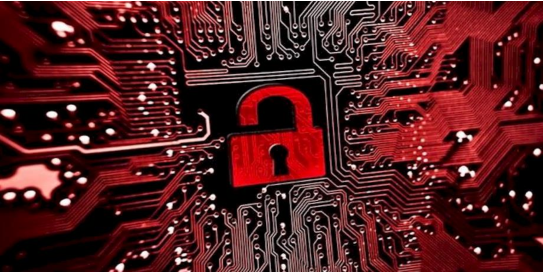
\includegraphics[width=5cm]{Tex/Pictures/chapter_head_1.pdf}}; 
\end{tikzpicture} 

\vfill
\endgroup


  % Book Cover
%----------------------------------------------------------------------------------------
%	COPYRIGHT PAGE
%----------------------------------------------------------------------------------------

\newpage

~\vfill
\thispagestyle{empty}

\noindent {\Huge\ccbyncndeu}\\ 

\noindent 2020 EDUF@CTION PUBLICATION (CC-BY-NC-ND)\\ % Copyright notice

%\copyright\ 

\noindent C\edoc est issu des supports de notes du cours SEC 101 \\ du \uCnam \\
ISBN-13: 978-1984901149 \\
ISBN-10: 1984901141 \\
Tous droits de reproduction, d’adaptation et de traduction,\\
intégrale ou partielle réservés pour tous pays.\\
L’auteur est seul propriétaire des droits et responsable du contenu de cet ouvrage.\\

\noindent \textit{Imprimé en Janvier 2020 \\ \printer} % 

%\chapter{Introduction}
\label{chapter:introduction}

\emph{An introduction... \cite{example-article}}


%----------------------------------------------------------------------------------------
%	TABLE OF CONTENTS
%----------------------------------------------------------------------------------------

%\usechapterimagefalse % If you don't want to include a chapter image, use this to toggle images off - it can be enabled later with 

 
	\usechapterimagetrue
	\chapterimage{../Tex/Template.inc/BookModel/BookPictures/chapter_head_1.pdf} 

\pagestyle{empty} % Disable headers and footers for the following pages

\tableofcontents % Print the table of contents itself

\cleardoublepage % Forces the first chapter to start on an odd page so it's on the right side of the book

\pagestyle{fancy} % Enable headers and footers again


%-------------------------------------------------------------
%               FR CYBERDEF SECOPS BOOK
%              $File : MyBookCyber.tex
%                             2020 eduf@ction
%-------------------------------------------------------------
% 								BOOK FILES
%-------------------------------------------------------------

%-------------------------------------------------------------
% 								PART 0
% 							Introduction
%-------------------------------------------------------------

\part{Cyber-généralités}
%-------------------------------------------------------------
%               FR CYBERDEF SECOPS BOOK
%                              $File : part0.tex
%                             2020 eduf@ction
%-------------------------------------------------------------
% 								BOOK FILES
 %	PART 0 : introduction et généralités
%-------------------------------------------------------------

%----------------------------------------------------------------------------------------
\chapterimage{Tex/template.inc/BookModel/BookPictures/chapter_head_2.pdf} 
%----------------------------------------------------------------------------------------

\chapter{Introduction}

	% Chap-Intro-gen.tex
% Introduction générale au cours SEC 101

\section{Avant propos }

Chaque jour, la presse se fait l'écho d'attaques et de piratages informatiques, de fragilités découvertes dans les produits et services incluant des codes logiciels, de vols de données. ou de divulgations d'informations sensibles.
Derrière ces incidents, nous découvrons des menaces de tout ordre, actions criminelles, étatiques, hacktivismes. Construire des systèmes surs, les protéger et les défendre, dans une société en ou d'accélérer la digitalisation est devenu un challenge quotidien pour des équipes spécialisées qui luttent contre ces menaces. 
La cybersécurité est un domaine de mythes et de légendes. Ses activités plongent au plus profond de notre histoire avec des notions comme la course entre le méchant et le gentil, le gendarme et le voleur jusqu'au corsaire et au pirate, en n'oubliant pas les luttes secrètes entre les espions et le contre-espionnage. Une thématique qui résonne, donc comme un domaine de romans, qui se traduit toutefois par une réalité souvent moins réjouissante pour les équipes chargés de la cybersécurité dans les entreprises. Les métiers de la cybersécurité sont nombreux, pour certains très techniques, d'autres plus fonctionnels, juridiques, ou managériaux. 

La cybersécurité est une discipline transverse et interdisciplinaire à plusieurs titres :
\begin{itemize}
  \item nécessité de maitriser les nombreuses technologies des systèmes d'information ainsi que leurs zones de fragilités;
  \item nécessité de maitriser de nombreuses solutions de sécurité permettant de couvrir, en n'oubliant qu'elles aussi peuvent être fragiles (Cf. Certification et Qualification de produits de sécurité et Critères communs);
  \item nécessité de faire coopérer des métiers et des cultures différentes ;
  \item nécessité de gérer l'entreprise dans des cadres de conformité souvent complexes et coûteux.
\end{itemize}


\mode<presentation>{\picframe{../Tex/Pictures/img-4model}{Cybersécurité : un domaine hollistique}{0.9}{lb_4model}}

Ces métiers concourent tous à une seule et même mission, : assurer la continuité de la mission ou du service en préservant le patrimoine de l'entreprise contre toute menace dans l'environnement numérique.

%\section{les grands cyber-risques}

% les grzands typologies de menaces liées au politique,, au vols, à la guerre écononiques" : Chnatage, Ilmages, Vole, Continuité d'activité ... manipulation, esionnage ...

% Les cyberrisques dépenade de la cibles, et souvent la cibles ets liée à l'attaquant

%\section{les vecteurs cyber}

\section{Les axes d'une cybersécurité intégrée}

% ajouter le joke sur les corsaires et une hallebarde

La cybersécurité dans une entreprise est donc une co-activité d'hommes de l'art.  C'est aussi un domaine en perpétuelle évolution, soutenu et contraint par des lois, des règlements , des normes, des méthodologies, et de technologies spécialisées.  Il nécessite pour être efficace d'être orchestré pour maintenir en condition de sécurité une organisation dont le périmètre peut être complexe.

Il y a de nombreuses manières d’aborder la cybersécurité au sein de l’entreprise, et nombreux ouvrages spécialisés en détaillent les concepts et les méthodologies. Nous avons toutefois délibérément choisi ici de confronter, si ce n'est corréler, dans un seul support, trois domaines qui apparaissent souvent dans la littérature comme des domaines d'expertise différents : la gestion des risques , la gouvernance de la cybersécurité, et la cybersécurité opérationnelle. 

Nous avons donc fait ce choix de structurer notre approche suivant le prisme de la cyberdéfense d'entreprise avec une analyse en trois axes majeurs qui résument les difficultés dont relève cette discipline holistique \cite{sch13}. 



% begin PRZ===================
\begin{frame}<presentation>{Les 3 axes de la cybersécurité}
	\begin{itemize}
 \item \tb{l'analyse des risques} informatiques sur les actifs les plus sensibles de l'entreprise avec les difficultés d'identifier la sensibilité de ces actifs et les menaces qui pèsent sur l'environnement ;
\item la structuration des \tb{politiques de sécurité} des systèmes d'information pour des architectures de sécurité de confiance, dans des systèmes d'informations complexes, intégrant des services dans le cloud, des technologies obsolètes et des politiques de sécurité sédimentées ;
\item la construction et l’organisation d'une \tb{sécurité opérationnelle} vue sous un angle d'anticipation et de veille, de détection, et enfin d'alerte et de réponse aux attaques, nécessitant une activité continue avec des ressources de plus en plus expertes et avec des outils plus \g{pointus}.
\end{itemize}
\end{frame}
% end PRZ====================

%\rem{Politiques : le monde de la reflexion, Stratégies le monde l'action}




\mode<all>{
\picframe{../Tex/Pictures/img-cycle}{Processus Cyber d'entreprise}{0.9}{lbl-cycle}
}

La figure \ref{lbl-cycle} présente la dynamique avec laquelle nous avons structuré dans c\edoc.


De  \head{l’analyse de risque}, nous pouvons déduire et/ou modifier des politiques de sécurité adaptées. 
Sur la base de l’existant, il est alors possible d’adapter ou simplement de mieux utiliser ou configurer les architecture techniques et organisationnelles pour définir un niveau de protection attendu.
Il y a malheureusement toujours un écart entre les mesures de sécurité souhaitées et la réalité des mesures déployées. Que ce soit des défauts de configuration, des délais de mise en place plus longue prévu, le système n’est que très rarement au niveau décrit dans les éléments de spécification ou les documents d'assurance sécurité.
Mesurer ce niveau, analyser les écarts et remédier relève d’un des grands thèmes de la gouvernance sécurité. Il reste à lui seul un consommateur à plus de 30\% des charges d'activité de cette gouvernance.

Après avoir définit des \head{politiques de sécurité} et mesurer leur déploiement dans l’environnement de l’entreprise, il n’en demeure pas moins que l’ennemi est toujours à ses portes et de plus en plus souvent. Il arrive à pénétrer le périmètre de sécurité.
Non pas que les barrières et filtre de l'entreprise ne sont plus efficaces mais simplement parce que l'attaquant change plus souvent de stratégie que l'entreprise de politique. La sécurité se doit d'être plus dynamique.
L’entreprise doit faire face à des attaquants qui ne raisonnent pas sous forme de politiques d’attaque, mais en stratégie d'action. L’entreprise doit raisonner aussi de la même manière pour se défendre. C'est à ce titre que l'on parle de stratégie de Cyberdefense.
C'est avec stratégies de \g{cyberdéfense} que nous aborderons les moyens organisationnels et techniques à mettre en place.

Vous trouverez  dans ce document une terminologie qui peut être certaines fois éloigné des expressions classiques de la sécurité informatique. \\
J'ai choisi de d'utiliser et mixer sans trop de complexes des termes et concepts issus du monde militaire (renseignement, tenir une position, infiltration …) et de nombreux autres issus de l'univers médical (infection, épidémie, comportement).\\ Ces incursions dans les analogies d'autres champs professionnels, bien que présents pour illustrer certains concepts, n'en demeurent pas moins justifiés par leurs usages de plus en plus répandus dans le monde de la cybersécurité. Par ailleurs, les termes sécurité, et cybersécurité pourront être utilisés indifféremment dans le corps de ce document.

\section {Transformation numérique}

% Les causes de la complexité

La cybersécurité est devenue en quelques années un axe fondamental dans la prise en compte de ces nouveaux risques sociétaux qu'apporte l'informatique au cœur de chaque activité sociale, économique ou politique. \\

%Quelque que soit le niveau d'impact  --- personnel, entreprise, Etatique, 
Les  transformations digitale d'une grande partie des acteurs économiques apporte de nouveaux risques. Les modifications des conditions d'utilisation des technologies dans les grises comme celle du COVID-19 engendrent aussi de risques globaux réduisant les frontières entre les espaces professionnels et les espaces privés.

Le législateur s'en est saisi depuis bien des années avec de nombreuses réglementations et lois permettant de protéger en particulier, le citoyen et l'Etat.

On notera en particulier dans cette évolution du cadre réglementaire,  la protection des données personnelles, mais aussi la protection des systèmes  en lien avec la protection de la nation avec la dynamique de Cyberdéfense soutenue par les différentes lois de programmation militaire. L'entreprise se trouve quant à elle prise en sandwich entre les exigences de l'état et les désirs de liberté que défend le citoyen. Il faut aussi noter que le citoyen est souvent un salarié et son rôle dans la cybersécurité de l'entreprise peut soulever des problématiques complexes.\footnote{Lanceurs d'alertes, comportements déviants des utilisateurs légitimes}
 
Se sentir en sécurité dans un monde de transformation digitale c'est bien entendu disposer des moyens de se protéger et protéger son patrimoine, que ce dernier soit ou non informationnel, mais aussi de le défendre en continue. Il est moins de moins en moins accepté de le protéger, en érigeant des murs épais, solides et supposés infranchissables. L'entreprise a besoin de faire circuler rapidement les savoirs, de partager largement des informations entre les salariés, les clients, les citoyens, les fournisseurs...


Il est donc nécessaire de correctement définir les biens vitaux ou essentiels pour y mettre les meilleurs moyens pour les défendre. Par ailleurs comme toute activité protégée et défendue qui peut subir des dommages, il est important de structurer l'activité numérique d'une entreprise ou d'une organisation pour pouvoir fonctionner en mode dégradé, et revenir à la normale en moins de temps possible.


Entre une maitrise des risques cyber et une capacité de se défendre et réagir, il est nécessaire de disposer déjà d'un bon niveau de protection adaptée aux enjeux du numérique. Il existe de nombreuses définitions de cette cybersécurité.

Pour ma part je vous propose de poser pour la suite de mon propos, une définition simple, qui a ses détracteurs mais qui résume en une pseudo équation la manière dont nous traiterons ce domaine dans c\ecours. \\
\begin{nota}[Une définition de la cybersécurité]
\begin{align}
Cybers\acute{e}curit\acute{e} \cong Cyberprotection\oplus Cyberd\acute{e}fense \oplus Cyberr\acute{e}silience
\end{align}
\end{nota}


% begin PRZ====================
\begin{frame}<presentation>{Une définition de la cybersécurité}
\begin{align}
Cybers\acute{e}curit\acute{e} \cong Cyberprotection\oplus Cyberd\acute{e}fense \oplus Cyberr\acute{e}silience
\end{align}
\end{frame}
% end PRZ====================

% begin PRZ====================
\begin{frame}

La cybersécurité est l'enchainement opéré, organisé, documenté, piloté, optimisé de trois environnements d'ingénierie :
\begin{itemize}
 \item \tb{Protéger} l'environnement par les mesures et solutions technologies adaptées au niveau de risque que l'entreprise est prêt à prendre; 
 \item \tb{Défendre} les actifs les plus sensibles de l'entreprise en surveillant et combattant la menace (y compris l'image de l'entreprise);
 \item assurer \tb{la continuité et la reprise d'activité} de l'entreprise face à tout incident rendant indisponible tout ou partie d'une fonction essentielle de celle-ci.
\end{itemize}

\end{frame}
% end PRZ====================

La Cybersécurité c’est donc avant-tout la mise en place de mécanismes de protection des biens et des processus numériques sensibles. C’est historiquement avec cette premiere dynamique que l’entreprise déploie des solutions de sécurité. 

Toutefois, malgré ce niveau de protection et souvent les lourds investissements réalisés dans des composants de sécurité périmétrique, l’entreprise peut se faire surprendre avec des attaques contournant ces mesures. Face à ces attaques, l’entreprise découvre que la solidité de l’entreprise n’est pas directement lié aux investissements sur les systèmes de protections. Il lui faut anticiper les menaces, les détecter non seulement sur son périmètre mais aussi dans l’écosystème de l’environnement les menaces potentielles. Ces menaces exploitent des vulnérabilités qu’il convient de détecter en amont.

Malheureusement, malgré ces mesures de protection et de défense qui permet de réagir vite et efficacement, il arrive que des attaques informatiques arrivent à leur fin. La capacité de l’entreprise à revenir à une situation normale, avec un contexte assaini est un critère dont un chef d’entreprise appréciera la valeur qu’après un incident.

% ajouter l’equation du risque dans le texte du RISQUE

Il fut une époque pas si lointaine, ou dans l'évaluation de la probabilité d'une attaque, l'analyste consacrait du temps. Aujourd'hui bine que ce paramètre continue quand même à être pris en compte, l'analyste positionne cette probabilité à 100\%.  (cf. figure \ref{lbl-riskassess})

% I M A G E -----------> 


\mode<presentation>{\picframe{../Tex/Pictures/img-risk-assess}{le cyber-risque}{0.9}{lbl-riskassess}}

 Car l'ensemble des experts du domaine est globalement en accord sur la posture que doivent prendre les entreprises et les organisations : \g{Le temps n'est plus de savoir si on sera attaqué ou pas, mais plutôt de savoir quand et comment on le sera}, qui concrètement se résume à la certitude que tout incident de sécurité peut se produire.
 
Dans les modèles d'analyse de risque et d'évaluation de la cybersécurité, l'analyste se positionne aujourd'hui du point de vu de l'attaquant. Ce regard lui permet de mieux comprendre la menace comme équation duale du risque, mais vu de l'énergie dépenser par l'attaquant et du risque qu'il prend. (cf. figure \ref{lbl-riskjail})



\mode<presentation>{\picframe{../Tex/Pictures/img-risk-prison}{La menace : une vision de l'attaquant}{0.9}{lbl-riskjail}}


\section{sécurité du système d'information}

Le système d'information est au coeur de ce \g{monde digital }, et il est le lieu d'activités humaines très denses, permettant à des utilisateurs de réaliser leurs activités, professionnelles ou privées, à l'aide de processus informatiques et de services. 

Ces activités doivent de plus en plus faire face à tout un système d'agression orchestré par des attaquants non seulement humains mais aussi\g{automatiques}. On observe aujourd'hui une multitude de situations critiques, incertaines dont l'occurrence quasi quotidienne provient de phénomènes variés, humains (isolés, en réseau,…), physiques et/ou technologiques. Parmi ces difficultés qui profitent aux pirates informatiques il y a de nombreuses failles ou fragilités que nous découvrirons, provenant des systèmes du SI sans lesquelles ils ne pourraient exploiter leurs attaques. Ces phénomènes sont une menace pour les conditions de sécurité du système d'information.

\subsection{Les fonctions SSI de gouvernance}

Au sein des grandes entreprises, il existe de nombreuses fonctions ou missions pour gouverner, piloter cette sécurité numérique.

%----begin FRAME-------
\mode<presentation>{\texframe
{SSI : Responsabilités}
{les métiers}
{
\begin{itemize}
 \item \head{Le gestionnaire de risque} ou \UKword{Risk Manager} qui porte l'animation de la gestion des risques dans les projets ou dans l'entreprise;
\item \head{Le responsable sureté / sécurité } généralement responsable de la sécurité physique ou sein de l'entreprise (vol, intrusion physique, contrôle d'accès). Il endosse le plus souvent la responsabilité des biens et des personnes;
\item \head{L'audit et le contrôle} : Au sein des grandes organisations, il peut exister un service \g{indépendant} dont la mission est d'auditer et de contrôler les activités des services;
\item \head{Les RSSI} : Responsables de la sécurité des Systèmes d'Information;
\item \head{Les DSSI} : Au sein des grandes entreprises, les RSSI globaux ne dépendent plus trop de DSI, et possèdent le rang de directeur;
\item \head{Le DPO} : la dernière responsabilité apparue dans l'environnement de la sécurité (En France successeur du CIL , Correspondant Informatique et Liberté) (\UKword{Data Protection Officer}).
\end{itemize}
}}%----end FRAME-------


Nous ne présentons rapidement ici que ceux qui seront utilisés directement dans ce document et qui sont fortement en liaison avec la sécurité des systèmes d'information.

\subsubsection{Les DSSI et RSSI}

Au sein de l'entreprise, il est important que quelqu'un porte la charge de suivre ces conditions de sécurité. C'est le rôle du RSSI (Responsable de la sécurité des systèmes d'information), ou DSSI (Directeur de la sécurité des systèmes d'information).
La mission de ce RSSI d'entreprise est de protéger son Système d'Information (SI), de le mettre dans une posture d'amélioration continue tant de son système de protection que de son système de défense. Le RSSI n'est pas seul pour assumer ces missions, à tous les niveaux de l'entreprise, s'organise des fonctions de sécurité tant au sein de la DSI (auquel est souvent rattaché le RSSI), qu'au sein d'autres activités de l'entreprise. 

\subsubsection{Le DPO}

A partir de mai 2018, une responsabilité plus juridique liée à la protection des données a été rendue plus visible avec la nécessité de disposer d'un DPO en entreprise (Data Protection Officer) héritier en France du Correspondant Informatique et Liberté \textit{CIL}.
Nous n'aborderons pas la fonction, les missions et la dynamique de responsabilité du DPO ici. Il faut toutefois que cette fonction possède de nombreux recouvrements dans la chaine de gouvernance du risque \g{informatique} auprès des directions d'entreprise. Orienté vers la protection des données à caractère personnel, le tropisme de la fonction DPO peut conduire certaines structures à oublier des pans importants des risques numériques comme :

\begin{itemize}
	\item la protection du patrimoine informationnel. (Espionage industriel).
	\item la protection des systèmes d'information contre risques de ruptures de services (Continuité d'activité)
\end{itemize}

\subsubsection{L'officier de sécurité de défense}
Pour les entreprises traitant des informations classifiées de défense ou liées aux contraintes de la classification de l'état, il est indispensable de se doter d'une fonction OS de défense. Son rôle est de s'assurer de la conformité à l'Instruction Générale Interministérielle IGI 1300 pour le \g{Confidentiel Défense} et l'instruction Interministérielle II901 pour le \g{DIFFUSION RESTREINTE}.

Nous resterons donc dans le cadre fonctionnel de la Cybersécurité dans son volet protection des Systèmes d'information et gestion des risques numériques.
Quand nous aborderont des sujets en forte adhérence avec les dynamiques de la GDPR nous donnerons les liens et les indications adaptés pour les DPO.
Par exemple, nous aborderons l'usage des données nominatives collectées et traitées dans les SIEM, ou celle recueillis sur le DarkWeb etc ...
\begin{remark}
Consulter le site \url{www.cnil.fr} pour parfaire ses connaissances en matière de réglementation européenne sur la protection des données personnelles. 
\end{remark}

\subsubsection{Responsabilités SSI}

Le maintien des conditions de sécurité du système d'information des grandes entreprises nécessite un RSSI Central ou une fonction semblable rattachée à un niveau plus global de l'entreprise.
On découvre ainsi des RSSI rattachés à la direction des risques, la direction générale, au contrôle interne …\\
 Il n'y pas de rattachement bien définit. La couverture de responsabilité dépend grandement de la taille et de l'activité de l'entreprise, mais aussi de la maturité de celle-ci en matière de gestion de risque et de gouvernance. Il peut y avoir des RSSI par entité, par projet à l’intérieur d'une entreprise. Leur mandat est fixé en fonction des enjeux sécurité de ces entités ou ces projets. 

Le fin mot de l'histoire est le \g{R} de RSSI. Son domaine de responsabilité dépendra de son mandat pour assumer ce rôle de garant d'un environnement \g{ possédant } des bonnes conditions de sécurité.
La gouvernance de la sécurité, est au coeur du métier du RSSI. La discipline que pilote un RSSI dans l’entreprise se nomme GRC (Gouvernance, Risque et Conformité)

La notion de système d'information a profondément évoluée ces dernières années. Le périmètre des risques digitaux inclus maintenant des systèmes et services externes à l'entreprise. Beaucoup d'entre eux sous la forme de réseaux sociaux, de services cloud ouvrant par ailleurs le domaine de supervision à la téléphonie avec les smartphones et leurs applications professionnelles ou non.

Bien entendu en fonction de la taille de l'entreprise et de ses enjeux, on peut disposer au sein de l'entreprise de nombreuses personnes ayant une fonction de RSSI. 

Le métier est riche et dispose d'un spectre de responsabilité et d'activité très large en terme de poste on y trouve par exemple :

% FRAME beamer PRZ ------------------------------------
\mode<all>{\texframe{Fonctions RSSI}{différents métiers} 
{
\begin{itemize}
\item \textbf{RSSI d'entreprise} : Responsable de la sécurité de sa structure.
\item  \textbf{RSSI d'un département, d'une organisation intermédiaire} : A l'image d'un RSSI d'entreprise, il assure toute les taches de gouvernance, il applique et fait appliquer les directives et politique de sécurité aux équipes du département / division / structure intermédiaire, il déploie les actions décidée dans la chaine fonctionnelle sécurité
\item   \textbf{RSSI d'un contrat, d'un projet contractualisé (Security Manager)} : Responsable de la sécurité du  déroulement d'un contrat. Souvent lié à un plan d'assurance sécurité, le RSSI contrat se doit d'assurer pour le client ou pour le fournisseur le suivi des exigences de sécurité du contrat.
\end{itemize}
}} % end FRAME.........................................................


\mode<all>{\texframe{Fonctions RSSI}{suite}
%. . . . . . . . . . . . . . . . . . . . . . . . . . . . . . . . . . . . . . . . . . . .
{\begin{itemize}
	\item \textbf{RSSI Projet} : La responsabilité sécurité couvre le projet. Le RSSI on parle souvent de \g{security by design}. La responsabilité dans ce type de poste recouvre l'intégration de la sécurité dans le système, le suivi des indicateurs définis (contractuels, ou réglementaires), la remonté des indicateurs de suivi de sécurité à la MOA (Maitrise d'ouvrage), la prise de décision autour des choix de sécurité ....
	\item \textbf{RSSI Produit / Service} : Au delà de ce qui est fait pour un projet, le RSSI produit a en charge de gérer la sécurité opérationnel c'est à dire Maintenir la sécurité de son produit ou de son service.
 \item \textbf{RSOP} : Le responsable sécurité opérationnelle, est souvent une RSSI dépendant d'une DSI, il est généralement et dans beaucoup de d'entreprise de taille moyenne le RSSI technique. Il assure opérationnellement la mise en place technique des politiques de sécurité et maintien en condition de sécurité l'ensemble de l'environnement informatique. Il est aujourd'hui au coeur de la sécurité opérationnelle face aux attaques et aux crises cyber.
\end{itemize}
}} % end FRAME.........................................................


\subsection{Conditions de sécurité}

Les conditions de sécurité représentent les propriétés fondamentales du SI, appelées : DICT (Disponibilité, Intégrité, Confidentialité, Traçabilité), qui favoriseront le fonctionnement optimisé du SI et éviteront l'avènement d'incidents de sécurité irréversibles ou même gênants pour son fonctionnement. D'un certain point de vue, les conditions de sécurité représentent le paramétrage du SI pour lequel le système fonctionne bien dans des conditions de sécurité \g{ connues et approuvées }

Ces fameux critères \textbf{DICT} ou propriétés de sécurité des systèmes d'information vise les objectifs suivants :
%-----------------------------------------
\begin{nota}[DISPONIBILITE]
le système doit fonctionner sans faille (arrêt, ou dégradation) durant les plages d'utilisation prévues et garantir l'accès aux services et ressources définies et installées avec le temps de réponse attendu.
\end{nota}
%-----------------------------------------
\begin{nota}[INTEGRITE]
Les données doivent être celles que l'on attend, et ne doivent pas être altérées de façon fortuite, illicite ou malveillante. En clair, les éléments considérés doivent être exacts et complets.
\end{nota}
%-----------------------------------------
\begin{nota}[CONFIDENTIALITE] Seules les personnes autorisées peuvent avoir accès aux informations qui leur sont destinées. Tout accès indésirable doit être empêché.
\end{nota}
%-----------------------------------------
\begin{nota}[TRACABILITE] (ou preuve ) : garantie que les accès et tentatives d'accès aux éléments considérés sont tracés et que ces traces sont conservées et exploitables.
\end{nota}
%-----------------------------------------
D'autres aspects peuvent aussi être considérés comme des objectifs de la sécurité tels que :
%-----------------------------------------
\begin{nota}[AUTHENTICITE]
l'identification des utilisateurs est fondamentale pour gérer les accès aux espaces de travail pertinents et maintenir la confiance dans les relations d'échange. On voit aussi dans la littérature la terminologie \g{ critères ACID (Authentification, Confidentialité, Intégrité, Disponibilité)}.
\end{nota}
%-----------------------------------------
\begin{nota}[NON-REPUDIATION]
La non-répudiation et l'imputation : aucun utilisateur ne doit pouvoir contester les opérations qu'il a réalisées dans le cadre de ses actions autorisées et aucun tiers ne doit pouvoir s'attribuer les actions d'un autre utilisateur.
\end{nota}

Dans un contexte d'activité économique dense et en perpétuel renouvellement, les conditions de sécurité sont aussi en perpétuelle évolution, c’est pourquoi nous parlons d'un cycle de vie vertueux au cours duquel les nouveaux paramètres tirent profit des expériences passées.  Ainsi, l’amélioration continue également appelée \g{ lean management} dans d’autres domaines (industrie, …) travaille-t-elle sur le cycle de vie des conditions de sécurité souvent appelé PDCA pour Plan, Do, Check, Act (Roue de Deming).\\
Ce cycle de vie doit néanmoins être maitrisé par le RSSI en place avec ses équipes, il faut co-produire ces conditions de sécurité, cette maîtrise est complexe, fortement dépendante du contexte de l'entreprise, c’est pourquoi elle doit être accompagnée d'une méthodologie rigoureuse et partagée qui constitue le savoir-faire de base du RSSI et de son équipe. Par ailleurs, parmi ces conditions, certaines sont universelles et d’autres propres à chaque entreprise. \\ Comme le montre le diagramme \ref{lbl-cycledevie}, il est possible aussi d’utiliser un cycle de vie sécurité de type projet, qui se rapproche par ailleurs de la manière dont nous avons structurer c\edoc. 

\mode<presentation>{\picframe{../Tex/Pictures/img-cyclevie}{Cycle de vie sécurité dans les projets}{0.9}{lbl-cycledevie}}


Dans cette optique, ce cadre méthodologie a été défini par le sous-comité 27 de l'ISO, par le bouquet de normes ISO 27x. Il s’agit également d'un ensemble de bonnes pratiques et de bon sens, que le RSSI peut suivre au travers de 3 Volets fondamentaux qui constituent les référentiels utilisés pour ce cours sur la cybersécurité. La norme 27001 est en particulier un cadre pour organiser la dynamique de la mise en condition de sécurité de l’entreprise et son maintien dans le temps. Cet environnement que le RSSI doit bâtir est le système de management de la sécurité (SMSI).

\\
Notre dynamique méthodologique est soutenue dans  c\edoc, par trois cadres normatifs : 
 
% FRAME beamer PRZ ------------------------------------
\mode<all>{\texframe{Cadres normatifs}{3 modèles du cadre}
%. . . . . . . . . . . . . . . . . . . . . . . . . . . . . . . . . . . . . . . . . . . .
{
\begin{itemize}
\item Identifier ses cyber-risques sur la base de méthodologies que l’on retrouve dans l’environnement ISO/CEI 27001/27005 mais aussi sur la méthodologie EBIOS de l’ANSSI (Méthode EBIOS RM en particulier); 
\item Elaborer une politique de cybersécurité sur la base des cadres ISO/CEI  27001 et 27002, en n’oubliant pas les architectures de sécurité et la sécurité des architectures associées ; 
\item Détecter en amont des attaques et savoir réagir à ses cyber-incidents en se basant sur ISO 27035 et sur la continuité d’activité avec l’ISO 22301 et 27031.
\end{itemize}
}} % end FRAME.........................................................


\begin{nota}[Pourquoi des normes dans c\edoc?]
L’objectif de c\edoc, n’est pas de présenter en détail un cadre normatif, mais bien de les utiliser pour ce qu’elles sont : des langages communs permettant d’appréhender une terminologie, des méthodologies, des outils. L’ISO 27001 comporte un grand nombre de normes (plus de 50…) qu’il convient de connaitre comme outils terminologiques et de référence. Leur maitrise nécessite une spécialisation le plus souvent demandée pour des métiers de conseil ou d’implémentation pour une certification.
\end{nota}

Ces documents définissent un cadre méthodologique et normatif pour définir, créer, élaborer maintenir, améliorer les conditions ou les critères de sécurité pour le fonctionnement du système protégé et surveillé. 
Ils permettent aux acteurs de l'entreprise évoluant autour du métier RSSI un cadre méthodologique ainsi qu’un \g{how to} du maintien en conditions de sécurité. C’est en particulier au travers de ces trois axes que la mission de RSSI repose. 
Le nombre d’entreprises prêtes à accueillir des spécialistes de ce savoir-faire est en forte augmentation car les PME/PMI ont pris conscience que la sécurisation de l’entreprise est devenu primordiale pour \g{survivre} dans l’écosystème digital de nos sociétés modernes. Les contraintes légales issues de la Loi de Programmation Militaire (LPM), de la Règlementation pour la Protection des Données Personnelles (RGPD), de la directive NIS nécessitent de disposer d’une vision globale et transverse tant technique, qu'organisationnelle ou humaine de la cybersécurité.

Nous tenterons donc dans le suite du cours, de vous donner des contextes d'usages de ces cadres normatifs indispensables pour aborder la cyberdéfense d’entreprise. 

\section{les enjeux légaux}

Beaucoup d'environnements normatifs sont issus de la pression des différents cadres législatifs sur le marché. Que ce soit avec la pression du grand public ou avec les enjeux stratégiques et économique des pays, ces lois organisent profondément les modes de gouvernance de la sécurité en entreprise.

\subsection{Quelques cadres législatifs d'influence}
Parmi les grandes lois qui ont influencé  le monde de la sécurité des entreprises ces dix dernières années :

\begin{itemize}
 \item En France, le cyberdéfense est largement orientée par les différentes \g{Lois de programmation militaire} avec des directives nationale de sécurité par grands domaines d'infrastructures vitales.
 \item En Europe deux grandes directives ont donné plus de responsabilité aux entreprises dans l'engagement sécurité avec GDPR et NIS qui sont déclinés en droits français via la CNIL, et l'ANSSI. On notera par ailleurs la montée en puissance dans la confiance numérique avec le cadre de certification européen.
 \item Aux Etats Unis, le \UKword{Cloud security Act}, a bouleversé la vision des risques numériques des états avec les potentielles nuisances liées à l'extraterritorialité de lois américaines
 \item En Russie et en Chine, plusieurs lois autour de l'usage d'internet interpellent les entreprises et en particulier celles du numérique sur la protections des données de leurs clients ou utilisateurs de leurs services.
\end{itemize}


\subsection{Le cadre de certification européen}

Le règlement établit un \link{https://www.ssi.gouv.fr/entreprise/reglementation/cybersecurity-act-2/le-cadre-de-certification-europeen}{cadre européen de certification}
 de cybersécurité pour harmoniser à l’échelle européenne les méthodes d’évaluation et les différents niveaux d’assurance de la certification, au sein duquel l’ENISA trouve toute sa place. Les certificats délivrés bénéficieront d’une reconnaissance mutuelle au sein de l’Union européenne (UE). 

\subsection{Cyberdefense et loi de programmation militaire}
Pour ceux intéressés par les contraintes et cadre généraux de la cyberdéfense au sein des lois de programmation successives (2008, 2013, 2019 ...) il est conseiller d'aller voir sur le site de l'ANSSI. Les différentes LPM ont fait évoluer le cadre réglementaire pour assurer à la France une capacité de défendre la continuité de l'état et des infrastructures vitales du pays \link{https://www.ssi.gouv.fr/entreprise/protection-des-oiv/protection-des-oiv-en-france/}{(Cf. Opérateurs d'infrastructures vitales)}.

	\section{Quelques organismes de référence}

La normalisation et la réglementation en matière de cybersécurité est riche mais certaine fois complexe.
Le plus simple pour s'enrichir de ces savoirs et surtout pour disposer des meilleurs informations à la sources autant \g{fréquenter} les sites internet institutionnels des organismes qui sont et continuent à être les points de  référence dans le domaine de cybersécurité.

De nombreux services étatiques et de normalisation possèdent des activités dites Cyber dans leur structures :

\begin{itemize}
    \item  Organismes français : AFNOR, Cert FR, CNIL, HADOPI, ANSSI, DGSE, DGSI, DGA/MI, Commandement de la cyberdéfense, C3N, OCLCTIC, BEFTI ...
  \item  Organismes internationaux : ISO, ETSI, CERT, Europo, lnterpol , ENISA , FIRST ...
  \item  Organismes étrangers : FBI, CIA, NSA, GCHQ, Unité 8200, Fapsi, The SANS institute, CISA ...
\end{itemize}

Je vous propose de donner quelques pointeurs sur des organismes experts  de référence du point de vue occidental par portée.

\subsection{International et Etats-Unis}

Au niveau international, on ne peut éviter les Etats-Unis, un pays qui oeuvre fortement dans le domaine des standards.

Le National Institute of Standards and Technology, ou NIST est une agence du département du Commerce des États-Unis. Son but est de promouvoir l'économie en développant des technologies, la métrologie et des standards avec l'industrie. 

\begin{itemize}
  \item \link{https://csrc.nist.gov/}{NIST COMPUTER SECURITY RESOURCE CENTER }
  \item \link{https://www.nist.gov/itl/fips-general-information}{NIST INFORMATION TECHNOLOGY LABORATORY}
\end{itemize}

On notera en particulier les référentiels cryptographiques du NIST et ceux liées à la cyberdéfense en particulier avec le \UKword{CyberSecurity FrameWork}

\subsubsection{SEI : Université de Carnegie Mellon}


Le Software Engineering Institute (SEI) est un centre de recherche-développement financé par des fonds fédéraux et placé sous le parrainage du département de la Défense des États-Unis ; son fonctionnement incombe à Carnegie Mellon University. Le SEI travaille avec des organisations pour apporter des améliorations significatives à leurs capacités d’ingénierie logicielle en leur fournissant le leadership technique afin de faire progresser la pratique de l’ingénierie logicielle. Le CERT Division du SEI est l’entité qui fait autorité et cherche à améliorer la sécurité et la résilience des systèmes et réseaux en particulier dans le domaine du logiciel(\link{https://www.sei.cmu.edu/research-capabilities/cybersecurity/}{Carnegie Mellon University - Cybersecurity research}).

\subsubsection{ISO}


L’ISO est une Organisation Internationale participant à l’élaboration de Standards. En ce sens la conformité à une norme a l’avantage d’être reconnu internationalement.
 
Les normes de la famille ISO 27000 permettent d’organiser et structurer la démarche de la gestion de la sécurité des systèmes d’information. Le schéma ci-dessous propose une représentation de la famille et leur positionnement : 

\begin{itemize}
  \item ISO 27001 décrit les processus permettant le management de la sécurité de l’information (SMSI)
  \item ISO 27002 présente un catalogue de bonnes pratiques de sécurité
  \item ISO 27003 décrit les différentes phases initiales à accomplir afin d’aboutir à un système de Management tel que décrit dans la norme ISO 27001
  \item ISO 27004 permet de définir les contrôles de fonctionnement du SMSI
  \item ISO 27005 décrit les processus de la gestion des risques
  \item ISO 27006 décrit les exigences relatives aux organismes qui auditent et certifient les SMSI des sociétés.
\end{itemize}

Nous aborderons dans le chapitre sur les politiques de sécurité, l'usage de ce cadre normatif dans la gouvernance globale de la cybersécurité au sein de l'entreprise

%TODO : Pourquoi se faire certifier ISO27K, les points durs.

\subsection{Europe}

Règlement (CE) n460/2004 du Parlement européen et du Conseil
du 10 mars 2004
instituant l'Agence européenne chargée de la sécurité des réseaux et de l'information
Agence européenne chargée de la sécurité des réseaux et de l'information
\link{https://www.enisa.europa.eu}{ENISA}

%BEGIN wikpedia
% TODO
\begin{itemize}
  \item Conseiller et assister la Commission et les États membres en matière de sécurité de l'information et les aider, en concertation avec le secteur, à faire face aux problèmes de sécurité matérielle et logicielle.
  \item Recueillir et analyser les données relatives aux incidents liés à la sécurité en Europe et aux risques émergents.
  \item Promouvoir des méthodes d'évaluation et de gestion des risques afin d'améliorer notre capacité de faire face aux menaces pesant sur la sécurité de l'information.
  \item Favoriser l'échange de bonnes pratiques en matière de sensibilisation et de coopération avec les différents acteurs du domaine de la sécurité de l'information, notamment en créant des partenariats entre le secteur public et le secteur privé avec des entreprises spécialisées.
  \item Suivre l'élaboration des normes pour les produits et services en matière de sécurité des réseaux et de l'information.
\end{itemize}
%END Wikipeida



\subsection{En France}

En France, la Cybersécurité est pilotée par un organisme dépendant des services du 1er Ministre. l'Agence National des Systèmes d'information (ANSSI).
L'ANSSI possède plusieurs rôles de fait. C'est un \g{régulateur} c'est à dire qu'elle définit des cadres réglementaires pour les entreprises mais c'est aussi une agence qui édicte des préconisations et des guides.

 \link{https://www.ssi.gouv.fr/agence/cybersécurité/ssi-en-france/}{Le site de l'agence} est riche en information et guide sur la cybersécurité.

Dépendant aussi de l'état, la \link{https://www.cnil.fr/}{CNIL} (Commission National Informatique et Liberté) est une autorité dont la mission est de protéger le citoyen. Avec l'avènement du règlement de protection des données personnelles, la CNIL a vu son pouvoir étendu.  

Il faut aussi citer l'AFNOR (l'Association française de normalisation), qui relaie en France la normalisation internationale dont l'ISO au de la de ses actions de normalisation purement française.

\section{Quelques associations et groupements professionnelles} 

A titre d'information, vous trouverez avec ces associations des points d'entrées sur 

\begin{itemize}
  \item \head{Club des Experts de la sécurité de l’Information et du Numérique}.
le \link{https://www.cesin.fr}{CESIN} est une association regroupant les RSSi d'entreprises, l'adhésion à cette association nécessite un parrainage et vous devez être RSSI.

  \item\head{Club de la sécurité de l'information Français}
\link{https://clusif.fr}{CLUSIF}, association qui propose de nombreux échanges sur la cybersécurité.

  \item\head{Club CyberEdu}
\link{https://www.cyberedu.fr}{CyberEdu}, issu des travaux sur la formation des enseignants en cybersécurité de l'ANSSI, l'association regroupe les écoles et les utilisateurs des travaux de CyberEdu.

  \item\head{Club HexaTrust}
\link{https://www.hexatrust.com/le-club/}{HexaTrust}, regroupe les éditeurs et fournisseurs de services français en cybersécurité.
\end{itemize}


	
\chapter{Attaques et attaquants}\index{Attaquants}

	%-------------------------------------------------------------
%               FR CYBERDEF SECOPS COURSE
%                                        SECOPS
%                                           Intro
%
%                       Introduction Cyberdefense
%                        Chap-Intro-attaquants.tex
%
%                              2020 eduf@ction
%-------------------------------------------------------------


Avant de nous lancer dans la mise en place de mécanismes de sécurité, de défense et de résilience, il est intéressant de revenir aux éléments essentiels d'une cyberdéfense d'entreprise. En effet, se protéger, se défendre, résister fait écho au concept d'attaque. Je vous propose important de définir et de caractériser une attaque et un attaquant. 

\utocomplete
	
	\utodo

\chapter{Enjeux pédagogiques}\index{Pédagogie}

	 
%----------------------------------------------------------------------
% 		S E C T IO N   PEDAGO
%----------------------------------------------------------------------
\section{Objectifs pédagogiques}
Il me semblait important d'apporter au lecteur un peu d'information autour des éléments pédagogiques de c\ecours. Vous trouverez donc dans ce chapitre quelques éléments sur les compétences, les métiers, le positionnement des activités de la cybersécurité.
En effet, c\ecours tente d'être une introduction à la cyberdéfense d'entreprise permettant à des acteurs du digital n'ayant pas ou peu de connaissance du domaine de repérer dans ce domaine à large spectre d'activités et de métiers.

Nous y abordons aussi les limites de c\ecours ainsi que des recommandations pour aborder le contenu avec plus de facilité pour ceux moins familiers du monde de l'informatique et des réseaux.

\subsection{Les compétences à acquérir}
A l'issue de c\ecours, vous devriez être en mesure de comprendre les mécanismes qui contribuent à la mise en place d'une organisation de cyberdéfense d'entreprise avec les grandes capacités nécessaires.  Pour les réaliser avec efficacité, il est nécessaire de positionner ces activités au sein des fonctions sécurité plus large. Les compétences acquises sont de diverses natures, mais globalement vous devriez être en mesure à un niveau de gouvernance et de pilotage de :  

\begin{itemize}
	\item Analyser les risques numériques pesant sur l'entreprise ou l'organisation ;
	\item Mesurer le niveau de sécurité de de l'environnement ;
	\item Auditer, conseiller, accompagner le changement ;
	\item Mettre en place une gouvernance efficace dans le domaine de la cybersécurité ;
	\item Déployer une politique de sécurité informatique et de cybersécurité et appliquer des méthodologies efficaces de renforcement et d'aguerrissement ;
	\item Comprendre l'intégration des solutions de sécurité suite à l'analyse de risque ;
	\item Gérer des situations d'incident pouvant aller à la crise cyber.
\end{itemize}
La complexité de l'entreprise, sa taille, sa dynamique de prise en compte des enjeux sécurité, sa culture, l'adhérence ou non aux technologies de l'information nécessitent le plus souvent des projets spécifiques adaptés et très contextualisés. Des sociétés de services assistent les entreprises pour auditer, construire, maintenir la sécurité de l'entreprise. Ce document a aussi pour objectif de fournir au lecteur des clefs de lecture pour encadrer et piloter de telles prestations dans le contexte de l'organisation. 


\subsection{Métiers et compétences } 
Il est complexe d'identifier les métiers de la cybersécurité vers lesquels ces compétences peuvent conduire. Il existe plusieurs modèles permettant de classer les métiers de la cybersécurité, et les compétences associées. Pour ma part,  j'ai retenu un modèle que j'ai proposé dans le cadre d'une GPEC (Gestion des emplois et compétence) dans chez un opérateur de services de cybersécurité. Ce modèle est centré sur une classification des outils technologiques utilisés par l'expertise. Issue plutôt de l'expérience, il ne reflète pas les dénominations des différents métiers ou fiche de poste que l'on trouve dans le domaine mais se centre sur les technologies de sécurité vu du côté des opérationnels. Ceci permet de décliner 5 grands domaines d'activité.

\upicture{../Tex/Pictures/img-metiers}{les  grands domaines de métiers}{0.9}{lbl_metiers}

Il y a en effet une grande différence de métier, de compétences entre un spécialiste de la gestion des accès  qui conduira l'intégration de système d'IAM  \footnote{Identity et Access Management} et un ethical hacker qui devra recherche des scenarii d'attaques potentielles sur un système. 

\upicture{../Tex/Pictures/img-metiers-risk2crisis}{les quelques grandes zones de métiers}{0.9}{lbl_risk2crisis}

Au delà de ces grands métiers du service, il est possible de positionner dans le cycle de vie des systèmes différents métiers de la cybersécurité. Les cultures, les objectifs, les technologies utilisées sont différentes mais concourent à la même finalité de protection de l'entreprise.

\upicture{../Tex/Pictures/img-metierslist}{les métiers dans le cycle de vie}{0.9}{lbl_metiersall}


%TODO : Métiers de l'intégration, des opérations, ...

% De l'importance de la TAXONOMIE, POSTE, METIER et COMPETENCE


Si vous souhaitez connaitre avec plus de détails les compétences nécessaires pour les métiers de la sécurité vous pouvez consulter deux grands sites de référence comme celui de l'\head{ANSSI} des 
 \link{https://www.ssi.gouv.fr/particulier/formations/profils-metiers-de-la-cybersécurité/}{métiers de la cybersécurité} ou celui du NIST sur le référentiel  \link{https://www.nist.gov/itl/applied-cybersecurity/nice/resources/nice-cybersecurity-workforce-framework}{NICE Cybersecurity Workforce Framework}


\subsection{Compétences et certifications}

Se former en cybersécurité, c'est pour celui qui travaille avec vous une certaine garantie de compétences. Dans le domaine de la Cybersécurité, la confiance dans les compétences d'un acteur du domaine se base dans le domaine des services en particulier sur la certification. Dans ces certifications, formes de perfectionnement dans un métier, on trouve généralement des  certifications EDITEURS (liés à des produits de sécurité), et des certifications d'associations professionnelles.

Cette dynamique de certification est une manière de compléter les formations initiales et sont  assez différentiante sur un CV dans le monde de l'entreprise en particulier celles qui travaillent dans un environnement international.



\subsection{Certifications éditeurs}

Nous verrons dans le chapitre sur les architectures de sécurité, les produits et services technologiques de sécurité. Une grande partie des fonctions de sécurité techniques est opérée par des produits (Logiciels, Appliances, Services Saas ...). La complexité de ces produits nécessite une formation spécifique pour en exploiter toute la richesse fonctionnelle.
Ces certifications sont par ailleurs souvent obligatoires pour travailler dans les métiers de l'intégration car elle permettent d'accéder au support des éditeurs. A titre d'exemple, nous pouvons citer deux acteurs connus qui disposent de mécanismes et programme de certifications à leurs produits. Ces certifications peuvent par ailleurs être délivrées par des tiers.


\head{Pour CISCO} \link{https://www.cisco.com}{Certifications de carrière CCNA, CCDA} 
%https://www.cisco.com/c/fr_ca/training-events/career-certification


\head{Pour Microsoft} \link{https://www.microsoft.com/fr-fr/learning/certification-overview.aspx}{Certifications }  pour  développeurs, Administrateurs, Architectes Solutions, Consultants.

\subsection{Certifications professionelles} 

La validation d'expertise par des certifications professionnelles est assez répandue dans le milieu de cybersécurité et en particulier dans les pays anglo-saxons. De nombreuses certifications existent, portées par des associations professionnelles, des groupes d'experts ou des entreprises de référence. Ces certifications nécessitent le plus souvent en plus de l'examen des années d'expérience et de pratiques prouvées.


% parler du fait qu'il faut des années d'experience et maintenir par des preuves

\head{\link{https://www.isc2.org/Certifications}{ISC}}  \UKword{the International Information System Security Certification Consortium} délivre des certifications reconnues et d'excellent niveau de reconnaissance.
Les deux principales sont :
\begin{itemize}
  \item CISSP : Certified Information Systems Security Professional
  \item SSCP : Systems Security Certified Practitioner
\end{itemize}


\head{\link{https://www.isaca.org/}{ISICA} } IT Audit, Security, Governance and Risk 

sous le nom de \UKword{Information Systems Audit and Control Association} cette association professionnelle existe depuis 1967, connue pour sont support à COBIT elle propose plusieurs certifications réclamée par les clients. 


\begin{enumerate}
  \item CISA: Certified Information Systems Auditor
  \item CISM: Certified Information Security Manager
 \item CGEIT: Certified in the Governance of Enterprise IT
  \item CRISC: Certified in Risk and Information Systems Control
\end{enumerate}

\subsection{Certifications Hacking} 

Il nous faut citer deux certifications très utilisées cans les métiers techniques de la cybersécurité et accessible sans expérience professionnelle à prouver.

\head{SANS Institute} (SysAdmin, Audit, Network, Security) et le GIAC \link{https://www.giac.org}{(Global Information Assurance Certification) }

\begin{itemize}
  \item Cyber Defense
  \item Penetration Testing
  \item Incident Response and Forensics
  \item Management, Audit, Legal
  \item Developer
  \item Industrial Control Systems

\end{itemize}


\includer{inc-certifs-hacking.tex}


%----------------------------------------------------------------------
% 				S E C T IO N   Structure 
%----------------------------------------------------------------------
\section {Structure pédagogique du cours}
Nous avons abordé le cours sur cheminement basé sur trois pivots :

\begin{itemize}
\item Pivot \head{RISQUES} : Pour défendre son espace  cyber  c'est-à-dire l'ensemble des produits, services, matériels, données utilisateurs utilisés par l'activité  économique de l'entreprise il faut non seulement que celui-ci soit identifié mais que les risques portant sur les éléments le constituant soient aussi clairement et consciemment pris en compte. C'est sur la base d'analyses des risques que sont construits les objectifs de sécurité d'un système. Il est bien entendu que de nombreux systèmes préexistent à une analyse de risque et que les objectifs de sécurité ayant conduit à la construction sont issus de  la sédimentation dans le temps de choix technologiques qui ne sont, par ailleurs rarement formalisés. Ainsi on remarque, que l'activité du l'évaluation des risques, ce que appelle en anglais  risk management  est porté plutôt par le domaine d'activités dénommé  information Security management  ou INFOSEC dans les pays anglo-saxons, mais que nous pouvons traduire  management de la sécurité de l'information.
\item Pivot  \head{ARCHITECTURE du SI}. Architecture de sécurité, défense en profondeur, politique de sécurité, usage du SI, IAM. L'analyse sera faite à partie des Politiques de sécurité pour construire ou améliorer la cybersécurité de l'entreprise. Définir des objectifs de sécurité relatifs aux risques,  positionner les politiques de contrôle, decfiltrage, et de gestion sur l'environnement  informationnel  de  l'organisation pour garantir la protection et la confiance sur les actifs sensibles. 
\item  Pivot  \head{MAINTIEN EN CONDITION DE sécurité}. Malgré toutes les précautions pour mettre en confiance un système d'information, il est illusoire d'une part de vouloir tout protéger, mais aussi de penser que les mécanismes de  protection résisteront à toutes les agressions. C'est donc en continu qu'il est nécessaire de veiller à la menace, de vérifier que de nouvelles fragilités n'apparaissent pas, de réagir au plus vite en cas de suspicion d'attaque ou de compromission.  Ce sécurité continue, dite dynamique est à la base du maintien en condition de sécurité de l'environnement digital de l'entreprise. 
A titre indicatif, on peut rapidement donner une matrice des classes de métiers associées à chaque pivot. Ceci permettra au lecteur de se focaliser peut être sur un chapitre qui le concerne un peu plus dans son quotidien.
\end{itemize}



%TODO  ajouter une description des classes d'activités 
% Image sur le cycle de vie

\begin{nota}[Les limites de l'exercice]
C\ecours est essentiellement une introduction à la cybersécurité sur son volet gouvernance (politiques et stratégies). Il permet de mettre en perspective les choix techniques, tant de protection et de défense face à une réalité économique, qui nécessite d'adapter protection et défense au niveau de risque. La décomposition sur ces 3 axes est un parti-pris qui évidement ne couvre pas dans le détail, l'ensemble des processus et actions du domaine de la cybersécurité. 
\end{nota}

Vu du côté du responsable sécurité, et donc des compétences acquises : Le RSSI se doit de  maitriser les risques de son SI vis à vis des conditions de sécurité, il est un auditeur en mesure : 

\begin{itemize}
  \item d'analyser les risques à partir de l'analyse des enjeux de l'entreprise, de ses actifs, de son existant, de la menace inhérente ou non à son entreprise ;
  \item de les traiter, les accepter ou pas, 
  \item de proposer les objectifs de sécurité à déployer pour construire les mesures de sécurité.
  \item Ceci conduit à l'objectif professionnel de cette partie :  Savoir comment démarrer la prise en compte de la sécurité des systèmes d'information dans une entreprise .  Il trouvera donc de bons outils théoriques et pratiques dans l'ISO 27005.
\end{itemize}


\begin{nota}[Dynamicité des risques]
Un RSSI ou son équipe conduit les analyses vis à vis de la menace. Il peut être conduit à lancer des audits.  Les mesures issus de ces audits permettent de définir sur les mesures en cours sont faibles, inutiles, vulnérables vis-à-vis des objectifs de sécurité. C'est ainsi qu'il est possible de conduire des analyses de risques sur des systèmes existants et de vérifier si les mesures actives sont compatibles avec les objectifs. On peut aussi constater qu'à ce titre une analyse de risque n'est pas figée dans le temps car les menaces ainsi que la sensibilité des actifs évoluent.
\end{nota}


Le RSSI se doit de maitriser les politiques de sécurité des systèmes d'information,  la PSSI étant le modèle de référence de façon à :
\begin{itemize}
\item planifier et produire ces conditions de sécurité ;
\item les adapter à l'entreprise ;
\item les mettre en œuvre au travers d'une architecture de sécurité propre à l'entreprise ;
\end{itemize}

Le lecteur trouvera un référentiel global dans l'environnement de l'ISO 27001 pour travailler autour du système de management de la sécurité.

Au delà de la gouvernance classique que l'on dit "de protection" de la cybersécurité d'entreprise qui se veut un moyen de deployer des mesures de sécurité (préventives, de formation, d'architecture), la sécurité opérationnelle apporte un nouveau lot de mesures et d'outillages liés à l'anticipation, la détection et la réponse aux attaques.

\begin{nota}[sécurité Opérationnelle] Lutte informatique défensive, sécurité dynamique, 
Cyberdéfense : plusieurs terminologies se côtoient pour évoquer des concepts, techniques, mesures, et méthodes souvent proches. 
\end{nota}


\subsection{Structure du cours}

L\ecours est donc organisé en 3 temps. Chaque temps est un module qui structure l'ensemble des éléments présentés dans le programme de l'unité d'enseignement dans une dynamique associée à la forme d'enseignement à distance et structurée autour de 3 cours issus des retours d'expérience d'experts du domaine de la Cybersécurité.  
\begin{itemize}
\item \head{Temps 1} : De l'analyse des risques à la déclinaison des objectifs de sécurité sur les essentiels de l'entreprise;
\item \head{Temps 2} : Des objectifs de sécurité à une politique de sécurité guidant et mesurant une sécurité implémentée (architectures et systèmes  de sécurité et sécurité des architectures et de systèmes d'information) ;
\item \head{Temps 3} : D'un système d'information \textbf{outillé, protégé et défendu} en matière de sécurité à une sécurité opérationnelle \textbf{maintenue, vigilante et  réactive}.
\end{itemize}

Ce document regroupe de manière plus détaillée les éléments la 3ième partie de l'unité d'enseignement que je nommerai pour la suite dans ce texte   VAR : Veille / Alerte / Réponse ,  les deux premières parties sont toutefois résumés dans deux chapitres préliminaires, permettant de positionner la démarche VAR dans un contexte global.

\subsection{Pour s'engager plus rapidement}

Du point de vue pédagogique, il est important de noter que vous pouvez aller vous initier au domaine de la sécurité des systèmes d'information avec les travaux de l'ANSSI de la \link{https://www.ssi.gouv.fr/administration/formations/cyberedu/contenu-pedagogique-cyberedu}{Mallette CyberEDU}. Cette mallette de cours contient les basics pour aborder la cyberdéfense d'entreprise.

Ces travaux sont issus d'un marché public de réalisation avec l’Université européenne de Bretagne  (qui regroupe 28 établissements d’enseignement supérieur et de recherche) et Orange pour la réalisation de livrables à destination des responsables de formation et/ou des enseignants en informatique.

l’ANSSI met à disposition cette mallette pédagogique qui contient : un guide pédagogique, un cours préparé d’environ 24 heures sur l’enseignement des bases de la sécurité informatique, ainsi que des éléments de cours pour les masters en informatique (réseaux, systèmes d’exploitation et développement).
Ces documents, réalisés par le consortium et l’ANSSI, sont disponibles sur le site de l'ANSSI.
 

\subsubsection {Pour le niveau BAC +3}

Pour ce niveau la mallette contient un syllabus pour le cours de sensibilisation et initiation à la Cybersécurité ainsi que 4 modules de support de cours.

\begin{itemize}
	\item module 1 :  notions de base
	\item module 2  :  hygiène informatique
	\item module 3 :  réseau et applications
	\item module 4 :  gestion de la cybersécurité au sein d’une organisation
\end{itemize}
Un quizz est également à disposition pour permettre d’évaluer les compétences acquises au fur et à mesure de l’avancé des enseignements.

\subsubsection{Pour le niveau Bac + 5} 

Pour ce niveau, des fiches pédagogiques par domaine permettent de découvrir :
\begin{itemize}
	\item la sécurité des réseaux
	\item la sécurité des logiciels
	\item sécurité des systèmes
	\item l’authentification
	\item la cybersécurité au sein des composants électroniques
\end{itemize}






%-------------------------------------------------------------
% 								PART 1 et 2 
% 							Risques et PSSI
%-------------------------------------------------------------

%\part[Gestion des risques]{Des cyber-risques \\à la politique de sécurité \\de l'information}
%
%----------------------------------------------------------------------------------------
%	PART (1 et 2) : Cybersécurité : Risque et Politique de sécurité
% Une seule partie pour la 1ere édition
%----------------------------------------------------------------------------------------
\chapterimage{../Tex/Template.inc/BookModel/BookPictures/chapter_head_2.pdf} 

%==========================
\chapter{La gestion des risques}\index{Risk Management}

\section{REDACTION EN COURS}

%==========================
\chapter{Politiques et architectures de sécurité}\index{PSSI et architecture de sécurité }

\section{REDACTION EN COURS}

%==========================
\chapter{Eléments de Cryptologie}\index{Cryptologie}

%-------------------------------------------------------------
%               FR CYBERDEF SECOPS COURSE
%              $Chapitre : Threat Management
%                 $theme : Architectures Sécurité
%     			 $File :  chap-secman-crypto.tex
%                             2020 eduf@ction
%-------------------------------------------------------------


A une époque où chaque jour la presse se fait régulièrement écho de pertes ou de vols de données, où l'on continue à investir dans la  protection des données personnelles, certains s'interrogent encore sur les moyens de protéger et partager de manière sûre son patrimoine informationnel. La cryptographie est une des disciplines de la cryptologie qui s'attache à protéger ces patrimoines en confidentialité, intégrité ou en authenticité. Il me paraissait intéressant de proposer en quelques mots,  le vocabulaire et les concepts. Si la cryptographie est un outil pour deployer des mesures de sécurité, c'est aussi un ensemble de techniques utilisées par les attaquant.  Au-delà des aspects mathématiques passionnants que nous ne traiterons pas ici,  seuls quelques usages et arcanes techniques sont présentés.

\section{Définitions}

 La cryptologie est par étymologie la science du secret. Elle regroupe la cryptographie, qui porte sur les moyens de coder et décoder les messages, et la cryptanalyse, qui permet de les déchiffrer (de manière non coopérative !).
Ces techniques remontent à la nuit des temps. Historiquement militaires et diplomatiques, elles sont devenues civiles avec l'avènement de technologies de l'information, dont la carte à puce \footnote{téléphonie mobile (SIM) et carte bancaire. } et l'internet.

Elles ont envahi à grande vitesse toutes les technologies numériques.\g{Signer, protéger, imputer, authentifier... } sont devenus des termes courants de cette vie numérique. On est toutefois surpris de l'usage, quelquefois un peu\g{dévoyé }, de certaines expressions.\g{Crypter } s'oppose à\g{décrypter }, mais si décrypter, c'est\g{décoder } sans connaître les secrets, crypter est humoristiquement enterrer  mettre en\g{crypte } ! Si les expressions\g{coder } et\g{décoder } sont régulièrement utilisées, celles préconisées sont\g{chiffrer } et\g{déchiffrer }. En France, au sein des armées, les acteurs du domaine se nomment d'ailleurs des spécialistes du chiffre \footnote{ARCSI : Association des réservistes du chiffre et de la sécurité de l'information - www.arcsi.fr}. Face à un spécialiste, du mathématicien cryptologue au commercial de services numériques de confiance, de nombreux termes se bousculent dans les discussions : algorithmes robustes de niveau militaire, clefs très longues, protocoles sûrs, certificats de confiance...

\section{Concepts}
Derrière ces arguments qui pourraient, au premier abord, paraître convaincants, il convient rapidement d'opposer une petite analyse terminologique et conceptuelle.

\subsection{Algorithmes}

Le nombre d'algorithmes mathématiques
(fonctions mathématiques) en cryptographie est presque aussi grand que le nombre de mathématiciens qui travaillent dans le domaine. Il faut y ajouter le nombre d'implémentations informatiques de chaque algorithme, sans compter les différents langages utilisés pour la même implémentation.
Quelques grandes révolutions ont eu lieu depuis le chiffre de César, mécanisme de chiffrement par décalage\g{alphabétique }
utilisé dans notre enfance, et celui de la machine allemande Enigma de la dernière guerre, avec des mécanismes de substitution dits polyalphabétiques. Ces évolutions et révolutions ont lieu chaque fois que ces fameux cryptanalystes trouvent ou entrevoient une solution pour casser ce chiffre... Une longue tradition dans cette course entre la cuirasse et le canon.


\subsubsection{Chiffrement à clefs secrètes} 
Ces premiers algorithmes dits symétriques ou à clefs secrètes ont été et restent centraux, car ils se révèlent très rapides. Le principe est que pour déchiffrer, il faut simplement la clef qui a servi à chiffrer, d'où le terme\g{symétrique }.
Une des grandes difficultés dans ces algorithmes est la combinatoire pour partager le secret. Si partager de manière sûre un secret entre deux ou trois correspondants est maîtrisable, le faire pour mille ne permet plus vraiment de parler d'une clef secrète ! L'histoire des célébrités technologiques retient des algorithmes comme DES, 3DES, IDEA, RC4 et le dernier réputé inviolé et issu d'un appel à projet du NIST\footnote{National institute of standards and technology.} et paru dans les années 2000 : AES256.

\subsubsection{Cryptographie à clefs publiques}
Le chiffrement asymétrique résout ce problème de la combinatoire, mais reste bien plus lent. Rendu célèbre par Alice et Bob, deux personnages illustrant les cours de cryptologie asymétrique, ce mécanisme utilise une paire de clés liées dites asymétriques : une clé publique et une clé privée. La clé publique est rendue publique et distribuée librement. La clé privée n'est jamais distribuée et doit être gardée secrète. Pour cette une paire de clés, les données chiffrées à l'aide de la clé publique ne peuvent être déchiffrées qu'avec la clé privée correspondante (donc si vous avez la clef publique de votre correspondant, vous pouvez chiffrer une information pour lui). Inversement, les données chiffrées à l'aide de la clé privée ne peuvent être déchiffrées qu'avec la clé publique correspondante. Cette caractéristique est utilisée pour mettre en œuvre la signature numérique.


\upicture{Tex/Pictures/img-crypto1}{Exemple d'une encapsulation asymétrique pour un chiffrement de fichier}{0.6}{lbl-crypto1}



\subsection{Fonction de hashage}

Les fonctions de hachage cryptographique (de l'anglais\g{hash }) sont présentes dans tous nos systèmes numériques. Ce sont des fonctions rapides à sens unique qui permettent de transformer tout bloc d'information de taille quelconque et une donnée de taille fixe souvent courte. Ce mécanisme, qui permet de prendre une\g{empreinte } des données, est à la base des mécanismes de signature, de contrôle d'intégrité et de stockage de mots de passe. Les algorithmes les plus connus sont md5, sha1 et maintenant sha256, sha512 nécessaires par les fragilités découvertes sur les premiers, car ces algorithmes sont aussi sujets aux attaques !


\subsection{Clefs}
Au cœur de la cryptographie, les clefs restent l'objet de toutes les attentions. Il est conseillé la lecture des quelques documents de référence de l'Anssi\footnote{Anssi : Agence nationale pour la sécurité des sytème d'information, services du Premier ministre.} sur les\g{mécanismes cryptographiques } \footnote{Annexe B1 et B2 du RGS V2 (Anssi : référentiel général de sécurité) : Mécanismes cryptographiques et gestion des clefs.} qui illustrent de manière pragmatique et concrète cette indispensable vigilance.
\subsubsection{Taille de clefs}
Un des débats dans l'usage de la cryptographie concerne la taille optimale des clefs. Ce sujet fait l'objet de nombreuses publications. Pour les algorithmes symétriques, 1 280 bits est la taille de référence (soient 2 puissance 128 possibilités). La notion de taille de clefs pour les algorithmes asymétriques est moins simple. Cela dépend des problèmes mathématiques sous-jacents. Pour le plus célèbre RSA\footnote{1978, apparition de l'algorithme à clef publique de Rivest, Shamir et Adelman (RSA).} (6), qui aura bientôt 40 ans, les experts considèrent qu'une taille de 2 048 est à l'état de l'art jusqu'en 2030. RSA est utilisé pour les transactions pour la carte bleue, les achats sur internet, les courriels sécurisés. Pour ceux basés sur le logarithme discret, la taille préconisée est de 200 bits, pour les courbes elliptiques de 256 bits. Il est donc important de spécifier les algorithmes pour comparer des tailles de clefs.
\subsubsection{Aléas et générateur d'aléas}
De nos jours, une bonne clef secrète est très rarement issue de notre cerveau (même un bon mot passe mémorisable est totalement perfectible sur le pur plan cryptographique)\footnote{Un mot de passe de qualité\g{cryptographique } devrait être d'au moins 20 caractères dans un alphabet de 90 symboles.}. Pour générer des clefs d'un bon niveau cryptographique, c'est-à-dire non sujettes à des biais de prédiction possibles, il est nécessaire d'utiliser un générateur de nombres aléatoires (GDA ou RNG : \g{random number generator}) de qualité cryptographique. Il est fondamentalement complexe de générer de véritables nombres aléatoires. Le processus de génération d'aléas doit comporter des sources fondamentalement aléatoires (bruit électronique, thermique dans des composants) combinées à des sources multiples (hash d'une zone mémoire...), le tout passé à la moulinette d'algorithmes de pseudo-aléas suffisamment imprévisibles. Ce fondamental de la cryptologie est un domaine de recherche à part entière. C'est aussi une activité industrielle autour des HSM (hardware security module) pour la génération rapide, le stockage et la protection des clefs primordiales pour les transactions numériques bancaires en particulier.
\subsubsection{Protocoles et formats}
De bons algorithmes, de bonnes clefs ne suffisent pas. Il est indispensable de s'assurer de l'ensemble des mécanismes qui vont permettre de garantir que\g{les secrets échangés } restent bien secrets. On parle de protocole d'authentification, de signature, d'échange de clefs (Kerberos, Diffie
Elmann, RSA...). C'est souvent au cœur de ces protocoles qui nécessitent une attention particulière en termes de robustesse et de preuve formelle que l'on trouve des vulnérabilités. Le format des données chiffrées (cf Fig. 2) est aussi une source de fragilité (cacher une partie de la clef en piégeant l'ordinateur, exploiter une vulnérabilité logicielle). Les solutions technologiques de chiffrement combinent pour des raisons de performance des mécanismes de chiffrement symétrique et asymétrique.
\subsubsection{Certificats}
Le terme\g{certificat électronique } est entré dans le langage courant du numérique :\g{Certificat machine, serveur },\g{certificat utilisateur }. à la base des usages des systèmes à clefs publiques, ce certificat contient la (les) clef(s) publique(s), des informations d'identification, des dates de validité, et un mécanisme de signature garantissant l'origine. Informatiquement ce\g{paquet } de données nécessite des standards de formats structurés interopérables comme le codage X.509 ou le stockage PKCS12.

% TODO Correction unicode à faire sur le texte suivant

%\footnote{ PKCS : Public-Key Cryptography Standards. (9) Moyen de cryptologie : Tout matériel ou logiciel conçu ou modifié pour transformer des données, qu'il s'agisse d'informations ou de signaux)}



%, à l'aide de conventions secrètes ou pour réaliser l'opération inverse avec ou sans convention secrète (loi n2004-575 du 21 juin 2004 pour la confiance dans l'économie numérique art. 38).}

\subsubsection{Certificats auto-signés !}
Une clef publique\g{valide } dans un système cryptographique de confiance, doit être signée par une autorité de confiance pour être vérifiée par la suite par son\g{usager }. Disposer d'une PKI ou faire certifier sa chaîne de confiance est complexe et coûteux. Le monde informatique fait donc largement usage de l'auto-signature, c'est-à-dire de la génération des clefs, sans chaîne de confiance partagée. Lorsque les logiciels sont permissifs sur ces usages, l'ensemble du système est fragilisé.

\subsubsection{IGC ou PKI}

Utiliser des mécanismes à clefs publiques nécessite donc l'utilisation d'un ensemble interopérable de confiance (algorithmes, protocoles, formats) permettant de générer les clefs (couple privée/publique), de les attribuer, de les signer (les certifier), de les distribuer, et de les révoquer (les supprimer de l'environnement de confiance). L'ensemble de ces mécanismes s'appelle une IGC (infrastructure de gestion de clefs) ou PKI (public key infrastructure). Ces outils logiciels et l'organisation globale sont indispensables à un usage structuré de confiance. Sans cette maîtrise des clefs, un système à clef publique peut s'effondrer. En effet, si des clefs de certification, ou des clefs privées d'utilisateurs sont compromises à la source, la résistance mathématique des algorithmes ou des protocoles ne vous garantira plus grand-chose... C'est dans cet esprit que sont nés les tiers de confiance, qui vous assurent que toutes les précautions sont prises pour protéger cette chaîne.



\section{De la confiance aux usages en entreprise}
Comme vous l'avez noté, un système cryptographique est un ensemble de briques (fig. 1) qu'il est nécessaire de contrôler pour définir un niveau de confiance de la chaîne. Si disposer d'outils à clefs publiques sans un IGC (PKI) se révèle fragile, disposer d'une IGC sans disposer d'une maîtrise des usages l'est autant...
En France, le terme de moyen (9) cryptologique est défini par loi sur la confiance numérique, mais il est à remarquer que, dans l'entreprise, il se conjugue différemment en fonction des interlocuteurs :


\begin{itemize}
 \item pour les équipes réseaux : la cryptologie est enfouie dans les méandres des protocoles des technologies des canaux sécurisés VPN, IPSEC, VPN, chiffreurs réseaux ;
 \item pour les équipes des services informatiques : le déploiement, la mise à jour des certificats sur des terminaux et des serveurs concentrent une bonne partie des problèmes opérationnels ;
 \item pour la bureautique et le poste de travail : les produits et les services pour chiffrer les données et préserver la confidentialité dans les messageries ou sur les supports (smartdevice, disques, USB, serveur de fichiers) sont complexes à choisir pour l'interopérabilité ;
 \item pour les métiers de l'entreprise comme les achats ou l'archivage probant, les enjeux d'authenticité, d'imputabilité et d'intégrité ainsi que la signature électronique nécessitent des travaux transverses à l'entreprise souvent coûteux.
\end{itemize}

\upicture{Tex/Pictures/img-crypto2}{ Les briques à vérifier dans la chaine de confiance}{0.6}{lbl-crypto2}


 Il est à noter, le point particulier du recouvrement des données chiffrées et du séquestre des clefs. Indispensable pour les malchanceux qui perdent leur clef privée ou par nécessité (départ de l'entreprise, réquisition sur des données...), la confiance dans celui qui possède cette capacité de recouvrement est un enjeu fondamental.
Acquérir et déployer un système cryptographique dans l'entreprise doit se baser sur un minimum de confiance dans
l'implémentation des briques. Il est important que ces produits aient été analysés, vérifiés par des tiers (entre le constructeur ou éditeur et l'utilisateur ou acheteur). On parle ainsi de certifications de produits au titre de la norme de l'Iso 15408 (critères communs), qualification de produits et de services par l'Anssi. Perturbant un peu l'écosystème et les frontières de gouvernance des DSI, l'usage des services dans le cloud nécessite de nouvelles technologies de chiffrement pour maintenir la confidentialité totale, mais autoriser quand même des traitements. Le chiffre homomorphe permet justement à un système tiers d'opérer des calculs sur des données chiffrées sans les déchiffrer et ainsi récupérer les résultats exploitables. Des solutions matures arrivent sur le marché depuis peu.


\subsection{De l'usure électronique au partage de confiance}

\subsubsection{Usure ou rupture cryptographique}
Si le temps n'est pas l'ami de l'archivage, il ne l'est pas non plus du chiffrement. Non par l'usure du support, mais simplement par la complexité d'une longue conservation des clefs, de l'érosion de la résistance des mécanismes. En outre, depuis des années, le terme\g{quantique } est apparu dans la littérature du domaine. Si la distribution quantique offre une transmission sûre de clef, l'ordinateur quantique pourrait apporter cette rupture que redoute l'industrie numérique, car capable de rompre la solidité des problèmes mathématiques sur lesquels repose une grande partie des mécanismes cryptographiques actuels.

La cryptographie quantique est un espace de recherche de cryptographie qui utilise les propriétés quantiques de la matière pour sécuriser les communications et protéger les données. Elle repose sur des phénomènes quantiques tels que l'intrication et la superposition, qui permettent de réaliser des calculs et des opérations de manière beaucoup plus rapide et plus efficace que les algorithmes classiques utilisés dans la cryptographie traditionnelle.

La cryptographie quantique est encore en développement et n'est pas encore largement utilisée dans les applications pratiques. Cependant, elle offre des avantages potentiels considérables en termes de sécurité et de vitesse de calcul. Par exemple, les algorithmes de cryptographie quantique pourraient être utilisés pour créer des clés de chiffrement plus sécurisées et pour effectuer des calculs complexes de manière beaucoup plus rapide que les algorithmes classiques.

Il est important de noter que la cryptographie quantique est également confrontée à des défis importants, notamment en ce qui concerne la stabilité des données quantiques et la difficulté à mettre en œuvre ces algorithmes de manière pratique. En outre, il existe des inquiétudes quant à la sécurité à long terme de la cryptographie quantique, car il est possible que de futurs progrès technologiques permettent de casser la confiance dans les chaines de confiance basée sur les algorithmes actuels de manière plus efficace.

En effet, si ces technologies sont pleinement mises en œuvre et deviennent largement utilisées, cela pourrait remettre en question la sécurité de nombreux systèmes de sécurité actuellement en place qui reposent sur des algorithmes de cryptographie classiques.

On peut citer les risques suivants

\begin{itemize}
  \item Rupture de la sécurité de la cryptographie classique : Si les algorithmes de cryptographie quantique sont mis au point et deviennent largement utilisés, ils pourraient être utilisés pour cracker les codes de cryptographie classique, mettant ainsi en danger la sécurité de nombreux systèmes de sécurité actuels
  \item Compromission de la confidentialité des communications : Si les algorithmes de cryptographie quantique sont utilisés pour chiffrer les communications, ils pourraient être crackés par des parties malveillantes, compromettant ainsi la confidentialité de ces communications.
\end{itemize}


\subsubsection{blockchain, Cyrpto-monnaies, NFT...}
Nous avons rapidement parcouru l'usage courant de la cryptographie en entreprise, mais de nouvelles révolutions des usages de la cryptographie sont déjà à nos portes. Après quelques années d'hésitation, la montée des\g{crypto-monnaie } comme Bitcoin donne une large expression aux mécanismes de signature pour assurer intégrité, traçabilité, imputabilité et modifie le rapport à la confiance\g{centralisée }. Dans l'émergence rapide de cette\g{décentralisation de la confiance }, quelques positions établies sont remises en cause. On notera en particulier une forme naissante d'ubérisation des chaînes de confiance, qui bouscule déjà le marché effervescent de la cybersécurité. Les chaines de confiance sont de plus en plus utilisé dans les cryto-monaies et NFT.

La cryptographie joue un rôle clé dans la sécurité et l'intégrité des blockchains en permettant de protéger les données et les transactions contre la modification ou la falsification.
Ces actifs numériques à caractère authentique sont basés sur ces blockchains. Une blockchain est une base de données distribuée qui permet de stocker de manière sécurisée et transparente ces enregistrements de données. Elle est composée de blocs de données qui sont liés les uns aux autres de manière sécurisée grâce à l'utilisation de cryptographie.

Chaque bloc de la chaîne contient des informations sur les transactions qui ont été effectuées, ainsi que des données sur les blocs précédents. Lorsqu'un nouveau bloc est ajouté à la chaîne, il est vérifié et validé par plusieurs ordinateurs dans le réseau, ce qui rend la blockchain très difficile à altérer ou à falsifier.

Les blockchains sont principalement utilisées pour stocker et transférer des cryptomonnaies, mais elles peuvent également être utilisées pour d'autres applications, telles que la gestion de la chaîne d'approvisionnement, la gestion des actifs, la gestion de la santé, etc. Elles offrent un niveau élevé de transparence et de sécurité, ce qui les rend particulièrement utiles dans les situations où la confiance et l'intégrité des données sont importantes.

Les cryptomonnaies sont des formes de monnaies numériques qui utilisent la technologie de la blockchain pour sécuriser les transactions et contrôler la création de nouvelles unités de monnaie. Elles sont décentralisées, ce qui signifie qu'elles ne sont pas émises ni gérées par une banque centrale ou tout autre organisme gouvernemental.

La cryptomonnaie la plus connue est probablement le Bitcoin, qui a été créée en 2009. Depuis, de nombreuses autres cryptomonnaies ont vu le jour, chacune avec ses propres caractéristiques et utilisations. Certaines sont conçues pour être utilisées comme moyen de paiement, tandis que d'autres sont plus axées sur l'investissement.

Les cryptomonnaies sont souvent utilisées comme moyen de paiement en ligne et sont acceptées par certaines entreprises et commerçants en tant que moyen de paiement. Cependant, elles restent controversées en raison de leur manque de réglementation et de leur volatilité, avec des fluctuations de prix importantes pouvant survenir en très peu de temps. En outre, leur utilisation a été associée à des activités illégales en raison de la confidentialité qu'elles offrent aux utilisateurs.

Les NFT (Non-Fungible Tokens) sont en effet des tokens numériques qui représentent de manière unique des actifs numériques ou physiques. Ils sont stockés sur une chaîne de confiance basées sur des blockchains, comme la blockchain Ethereum, ce qui leur confère une certaine forme de rareté et de valeur.

Les NFT sont  utilisés pour représenter des objets virtuels tels que des œuvres d'art numériques, des enregistrements de musique, des GIFs animés, des émoticônes, des personnages de jeux vidéo, etc. Ils permettent aux créateurs de ces actifs de monétiser leur travail de manière transparente et sécurisée, tout en offrant aux acheteurs la possibilité de devenir les propriétaires uniques de ces actifs.

Si les NFT sont de plus en plus populaires et suscitent beaucoup d'intérêt en raison de leur capacité à représenter de manière unique des actifs numériques, il est important de noter qu'il existe également des risques liés à l'achat et à la possession de ceux-ci. On note en particulier la confiance dans la sécurité globale dans ces blockchains ainsi que la stabilité et la liquidité du marché des NFT.








%-------------------------------------------------------------
% 								PART 3
% 				Sécurité Opérationelle
%-------------------------------------------------------------

\part[Sécurité opérationnelle]{Des stratégies de cyberdéfense \\à la gestion de crise}
%----------------------------------------------------------------------
%	PART 3 : Cyberdefense
%----------------------------------------------------------------------
\chapterimage{../Tex/Template.inc/BookModel/BookPictures/chapter_head_3.pdf} 
%---------------------------------------------------------------------

%==========================
\chapter{Introduction à la SECOPS}\index{SECOPS}

%-------------------------------------
% Chapitre
% Vulnerability Management
% Introduction
% File : chap-VTI-intro.tex
%--------------------------------------
\uchap{Chapitre introductif de la Partie 3 du cours SEC 101 (VTI-INTRO)}

\section{sécurité opérationnelle}

Après avoir construit une structure de sécurité cohérente sur les aspects de gestion des flux, de gestion des accès et des identités, et construit une gouvernance efficace sur la base de l'ISO27001, il est nécessaire maintenant de maintenir le niveau de sécurité de l'entreprise ou du système.

% begin PRZ==========================
\begin{frame}
\frametitle<presentation>{sécurité opérationnelle}
\framesubtitle<presentation>{Dans le cycle de vie}
% end header PRZ======================
On appelle quelque fois ce processus le \g{Maintien en Condition de sécurité} que nous pourrions positionner dans le RUN en utilisant  les termes anglo-saxons définissant le cycle des projets :

\begin{itemize}
 \item \textbf{THINK/DESIGN} : Des risques évalués à la politique sécurité pensée ;
 \item \textbf{BUILD}: De la politique de sécurité déployée à la construction d’une sécurité implémentée;
\end{itemize}
\end{frame}
% end PRZ ===========================


% begin PRZ==========================
\begin{frame}
\frametitle<presentation>{sécurité opérationnelle}
\framesubtitle<presentation>{l'activité RUN}
% end header PRZ======================
\upicture{../Tex/Pictures/img-thinkrun}{les phases du cycle de vie}{0.7}{lbl_thinkrun}

Et nous classons donc dans la dernière phase du cycle de vie : les activités d'exploitation de la sécurité, \textbf{RUN} : Des évènements de sécurité gérés à une \textbf{Cybercrise} maitrisée, que que certains appellent \textbf{SECOPS} : \g{sécurité Opérationnelle}.
\end{frame}
% end PRZ ===========================


% begin PRZ==========================
\begin{frame}
\frametitle<presentation>{Objectifs adapté aux finalités}
\framesubtitle<presentation>{de l'activité de l'entreprise}
% end header PRZ======================
Ce modèle se développe bien entendu en fonction des finalités de l'entreprise.

\begin{itemize}
    \item Soit nous sommes dans \textbf{une entreprise }et ces processus sont ceux mis en place pour s'assurer que  l'ensemble de actions sont prises pour maitriser les fragilités dont les vulnérabilités informatiques, détecter les menaces tant en anticipation que pendant des attaques (bruyantes, ou discrètes), et réagir pour maintenir l'activité et limiter l'impact.
    \item  Soit nous sommes \textbf{fabricant d'un produit ou d'un service}, et au delà des engagements sécuritaire de toute entreprise (cf. ci-dessus) des processus de \g{maintien en condition de sécurité} des produits et services sont à ajouter pour maîtriser les vulnérabilités, les correctifs et leur cycle de vie  (audit, communication, gestion des découvertes de fragilités par des tiers, rémunération de BugHunters ...)
\end{itemize}
\end{frame}
% end PRZ ===========================

% begin PRZ==========================
\begin{frame}
\frametitle<presentation>{sécurité opérationnelle}
\framesubtitle<presentation>{Une définition}
% end header PRZ======================
 Le terme de \g{sécurité opérationnelle}, est relativement jeune dans l’histoire de la sécurité des technologies de l’information. Le terme de SSI (sécurité des Systèmes d’Information) était né pour distinguer des disciplines qui s’attachaient à protéger l’information qui circulent dans les systèmes d'information de l’entreprise (cf. protection et classification de l’information) vis à vis de la sécurité des biens et des personnes. La sécurité des réseaux et la sécurité informatique ont été les précurseurs de la cybersécurité, le cyber recouvrant en un seul terme, les enjeux de sécurité liés au réseau et à l’informatique, mais plus largement à la sécurité de l'économie numérique.
\end{frame}
% end PRZ ===========================



Comme nous l’avons abordé, dans les chapitres précédents, la cybersécurité est un domaine vaste qui regroupe de nombreuses disciplines pouvant intervenir dans des cycles projets pour construire des systèmes sûrs et pour assurer la continuité d’activité et la protection des patrimoines dans l'entreprise. Il faut y ajouter aussi tout un espace de gestion des conformités (legislatives, réglementaires, normatives, contractuelles).
C’est plutôt dans un contexte d'opération sécurité au quotidien que l’on parle de sécurité opérationnelle. Ces activités opérationnelles supportent donc le maintien en condition de sécurité au quotidien de l’entreprise. En France, au sein des armées, on parle de lutte informatique défensive permettant de différentier les activités des Cyber-défense des activités de Cyber-protection. Ces activités sont à opposer à la lutte informatique\g{offensive} qui ne sera pas abordé dans c\ecours car elle relève de prérogative des états et non des entreprises. Nous aurons toutefois l'occasion d'aborder le \textbf{Hackback}, dans le chapitre sur la réponse à incident.
La sécurité opérationnelle ajoute par ailleurs à son périmètre de surveillance de l'intérieur de la zone de responsabilité de l'entreprise SI, réseaux sociaux, services cloud ...), celle extérieure à l'entreprise via des mécanismes de veille sur la menaces et de surveillance des compromissions potentielles. Nous pourrions évoqué l'image d'une cité où \g{Les murs sont épais et solides, les douaniers sont aux portes de la cité, la police doit toutefois veiller à la sécurité des biens et des citoyens dans la ville, car certains sont néanmoins des brigands. Quand à l'armée, elle veille aux frontières du pays informée pas des agents à l'étranger}.

On traitera donc cette partie avec une équivalence dans les terminologies suivantes :

% begin PRZ==========================
\begin{frame}
\frametitle<presentation>{Plusieurs terminologies, une dynamique}
% end header PRZ======================
	\begin{itemize}
		\item Maintien en condition de sécurité (MCS);
		\item sécurité opérationnelle (SECOPS);
		\item Lutte informatique défensive (LID);
		\item Cyberdéfense au sens de la cyberdéfense d'entreprise (CYBERDEFENSE).
	\end{itemize}
\end{frame}
% end PRZ ===========================

Le but de cette sécurité opérationnelle est d’être au coeur de l’action de la sécurité de l’entreprise. En effet, la sécurité de l’entreprise est une propriété multiforme. Elle est d’abord statique dans la mesure où elle correspond à un niveau de confiance dans l’environnement pour conserver la disponibilité, la confidentialité et l’intégrité de l’entreprise. Cette forme statique est souvent liée à la conformité de l’entreprise aux différents référentiels sécuritaires (ISO27000, GDPR, LPM, NIS ...), mais surtout aux objectifs sécurité de l'entreprise face à ses risques et aux exigences de sécurité des clients souvent inscrites dans des plans d’assurance sécurité (Cf. PAS). 
Elle est aussi dynamique car c’est aussi une propriété systémique qui mesure la capacité à anticiper les menaces, identifier les fragilités , détecter en temps réel les attaques et réagir à temps ou au pire disposer des capacités de revenir dans un état de fonctionnement compatible avec la survie de l’entreprise (Modes dégradés par exemple).
Le système évolue, faisant apparaitre ici et là de nouvelles fragilités, l’entreprise se transforme, vit, suscitant de nouveaux potentiels d’attaques. L’entreprise doit s’organiser pour disposer de fonctions opérationnelles adaptées et dédiées à cette activité. Ces fonctions nécessitent des savoirs, des savoirs-faire et de l’outillage. C’est l’ensemble de ces techniques que nous allons tenter d’aborder dans c\edoc.

Globalement, on peut remarquer que le cycle de vie est a prendre dans le sens inverse de notre présentation. Dans les entreprises moins matures en gouvernance de la sécurité, la dynamique de cette sécurité opérationnelle est la première visible et opérée. Dans l'entreprise va réagir le, plus souvent dans une dynamique de réponse immédiates aux problèmes de sécurité sans pour autant investiguer plus avant dans les fragilités globales. Les mécanismes de cybersécurité sont donc construits dans une entreprise peu mature dans le sens suivant :

% begin PRZ==========================
\begin{frame}
\frametitle<presentation>{Enjeux SECOPS}
% end header PRZ======================
	\begin{itemize}
		\item Répondre aux incidents de sécurité, tenter de répondre à la question : \g{qui nous attaque et pourquoi}; 
		\item Améliorer les filtrages;
		\item Couvrir les vulnérabilités découvertes;
		\item Rechercher les vulnérabilités existantes dans le périmètre de responsabilité ;
		\item Anticiper les attaques;
		\item Anticiper les risques informatiques;
		\item Anticiper les risques sur l'information;
		\item Anticiper la menace.
	\end{itemize}
\end{frame}
% end PRZ ===========================

\section{Lutte contre la menace}

La finalité de cette défense d’entreprise est de lutter contre ces attaques qui ne sont pas qu’informatique. L’attaquant peut utiliser des scenarii utilisant de nombreux vecteurs qui peuvent utiliser des fragilités organisationnelles ou humaines. On peut dire qu’une attaque est une fonction complexe, qui peut viser ou utiliser de nombreux facteurs internes et externes à l’entreprise. Ces facteurs constituent ce que certains nomment l’environnement numérique ou digital de l’entreprise. Cet environnement est globalement constitué de l’ensemble des outils, services, moyens informatiques ou réseaux utilisés par l’entreprise.
Mai 2017 a été un tournant dans la prise de conscience de la menace de la part des entreprises. Le Rançon-logiciel WannaCry a plus fait trembler les médias que les entreprises, mais a permis de faire comprendre au grand public les enjeux des menaces informatiques.


\begin{nota}[Paramètres d’une attaque]
\begin{equation}
Attaque = Fonction \left[ Fragilit\acute{e}s\,HOT\, Entreprise\otimes Gains\,Escompt\acute{e}s\,PF \right]
\end{equation}
\end{nota}

\begin{itemize}
	\item Fragilités HOT : Humaines, Organisationnelles, Techniques 
	\item Gains pour l'attaquant : Idéologiques, Politiques, Financiers, ...
\end{itemize}

On peut noter quatre grandes classes d’attaques informatiques \footnote{La majorité des attaques élémentaires peut être rangée dans ces classes}:

% begin PRZ==========================
\begin{frame}
\frametitle<presentation>{Grandes typologies des attaques numériques}
% end header PRZ======================
\begin{itemize}
\item Attaques \textbf{d’interception} d’information, vols par écoutes passives ou actives dans les flux transitant entre un émetteur et un récepteur;
\item Attaques par \textbf{déni de services}, généralement sur le réseaux : Ce type d’attaque est un atteinte à la DISPONIBILITE du système, basé souvent sur la saturation d’une capacité de traitement. Le système saturé dans l’exécution de certaines de ses fonctions, ne peut plus répondre aux demandes légitimes, car il est occupé à traiter d’autres sollicitations;
\item Attaques par \textbf{exploitation de failles }logiciels : Ce type d’attaque va utiliser une vulnérabilité, d’un système d’exploitation ou d’un logiciel pour exécuter du code malveillant. Ce code réalisera alors sa mission;
\item Attaques par \textbf{exploitation de défauts} de configuration : Ce type d’attaque utilise simplement un ou des défauts de configuration pour que légitimement l’agresseur puisse dérouler un scénario, qui pourra lui donner par exemple des droits particuliers pour conduire des attaques.
\end{itemize}
\end{frame}
% end PRZ==========================

Nous pourrions remarquer que ce nombre est relativement faible. Toutefois, la vrai difficulté réside dans la multiplicité des vulnérabilités, et des défauts de configuration. Les développeurs réalisent des logiciels possédant des failles (vulnérabilités), les utilisateurs ou les administrateurs déploient des systèmes en faisant des erreurs de configuration, ou ne les configurent que très rarement en pensant à la malveillance.

Les motivations des attaquants sont nombreuses, et leurs objectifs variés :

% begin PRZ==========================
\begin{frame}
\frametitle<presentation>{Motivations de l'attaquant}
% end header PRZ======================

\begin{itemize}
\item obtenir un accès au système pour s’y maintenir en attendant un opportunité ;
\item récupérer de l’information, secrets, données personnelles exploitables (en gros toutes information ayant de la valeurs)
\item récupérer des données bancaires ;
\item s'informer sur l'organisation (entreprise de l'utilisateur, etc.) ;
\item troubler, couper, bloquer le fonctionnement d'un service (les rançongiciels entre dans cette catégories) ;
\item utiliser le système d’un utilisateur, pour rebondir vers un autre système ;
\item détourner les ressources du système d’un utilisateur (utiliser de la bande passante, utiliser de la capacité de calcul) ;
\end{itemize}
\end{frame}
% end PRZ==========================

Bien entendu, il n’y a que très rarement un seul objectif, c’est la combinaison des méthodes d’attaques, des objectifs unitaires qui définissent globalement une mission ou un objectif final. L’exploitation de vulnérabilités au sein de l’entreprise va permettre le déploiement par l’attaquant d’un scénario.

\subsection{Politiques et Stratégies}

% begin PRZ==========================
\begin{frame}
\frametitle<presentation>{Politique vs stratégie}
% end header PRZ======================

\upicture{\upath/Pictures/img-cyclevie-pol-strat}{Positionnement de la sécurité opérationnelle}{0.9}{lbl_pol-strat}

\end{frame}
% end PRZ==========================

A partir des risques identifiés, l’entreprise a posé des politiques de sécurité qui ont permis de mettre en place des mesures de sécurité. Ces mesures sont d’ordre techniques avec des systèmes de sécurité, ou des SI avec des architectures particulières, mais aussi d’ordre organisationnel avec des procédures et des mécanismes à respecter.
L’ensemble de cette dynamique construit un niveau de sécurité qu’il va être nécessaire de maintenir dans le temps. Toutefois ce niveau de sécurité n’est pas suffisant pour une simple et bonne raison : la menace évolue, les vulnérabilités apparaissent (découvertes, ou créées), la valeur\g{marchande} des actifs d’une entreprise change aussi. 
Les occurrences de ces éléments de vie sont considérés comme des évènements qu’il convient de détecter avec suffisamment d’avance sur l’attaquant pour pouvoir le plus rapidement les prendre en compte.

La gestion des événements qui peuvent être un source de mesure de l’évolution du niveau de sécurité de l’entreprise est au coeur des stratégies de cyberdéfense. Ces évènements sont corrélés avec des sources provenant de deux processus particuliers qui seront décrit dans ce c\edoc.

% begin PRZ==========================
\begin{frame}
\frametitle<presentation>{Politique vs stratégie}
% end header PRZ======================
Il est à noter qu'un attaquant ne raisonne pas en politiques d'attaque face à une politique de sécurité, mais par des stratégies auxquelles il faut opposer aussi par des stratégies de défense, dont 

\begin{itemize}
\item Recherche des vulnérabilités : Processus qui permet de rechercher, découvrir, couvrir les vulnérabilités ou fragilités de l’entreprise ou ayant un impact sur l’entreprise que celles-ci soient techniques, humaines ou organisationnelles ;
\item Prévention de la menace : Processus qui permet de connaitre les menaces directes sur l’entreprise ou potentielles afin d’anticiper et/ou se préparer à un type d’attaque.
\end{itemize}
\end{frame}
% end PRZ==========================

C’est la confrontation entre les vulnérabilités, les menaces et la détection de l’activité de l’entreprise qui va permettre d’être efficace dans le processus de réponse. Il y a de nombreuses manière d’aborder la cyberdéfense d’entreprise.

C\edoc présente donc une dynamique de cyberdéfense en trois\g{volets }

% begin PRZ==========================
\begin{frame}
\frametitle<presentation>{3 volets d'une cyberdéfense}
% end header PRZ======================


\begin{itemize}
\item Gestion des vulnérabilités (\textit{Vulnerability Management and CERT}) : maitriser ses vulnérabilités mais aussi surveiller l’environnement technologique. 
\item Surveillance, Détection de la menace (\textit{Event and Threat Management}) : Analyser en temps réel l’environnement protégé mais aussi surveiller l’écosystème lié à la menace pour anticiper 
\item Gestion des incidents et réponse aux incidents (\textit{Incident Response – CSIRT}) : Réagir en cas d’incident et assurer la remédiation
\end{itemize}

\end{frame}
% end PRZ==========================


% begin PRZ==========================
\begin{frame}
\frametitle<presentation>{3 volets d'une cyberdéfense}
% end header PRZ======================
\upicture{\upath/Pictures/img-triangle}{Des 3 des volets de la sécurité opérationnelle}{0.6}{lbl_triptyque}

\end{frame}
% end PRZ==========================

Ces trois volets ne sont pas les seuls qui concourent à la cyberdéfense d’entreprise, mais ils en restent les trois faces principales. Il est à noter que ces trois volets correspondent aussi en France à trois référentiels de qualification de l’ANSSI des prestataires de services de cybersécurité au profit des entreprises. Ces labels sont obtenus par les entreprises qui respectent un cahier des charges rigoureux sur le plan de l'éthique, du professionnalisme, et de la compétence des experts intervenants. Il y trois cadres principaux de certifications sont :

% begin PRZ==========================
\begin{frame}
\frametitle<presentation>{Référentiels ANSSI}
% end header PRZ======================
\begin{itemize}
\item PASSI : Prestataire d’Audit de la sécurité des systèmes d’information ;
\item PDIS : Prestataire de détection d’incident de sécurité ;
\item PRIS : Prestataire de réponse à incident.
\end{itemize}

Ces trois référentiels définissent l’ensemble des exigences d’assurance pour\g{qualifier} des prestataires de services en cybersécurité sur ces trois thématiques. En effet, il serait en effet important de confier la recherche de ses vulnérabilités, leurs remédiations à des sociétés de confiance. 
\end{frame}
% end PRZ==========================
A ces 3 volets il ne faut pas oublier, le volet administration des briques informatique et de télécommunications de l’environnement de l’entreprise. C’est un volet que nous traiterons pas directement dans c\edoc pour se concentrer. sur les mécanismes de maintien en continue le niveau de sécurité de l’entreprise avec des mécanismes de veille, d’alerte et de réaction.


%TODO Leure et Hony Posts
%Leurres et Pots de Miel 
%Renseignement


\subsection{Stratégies d'action}

% Begin PRZ ===========================
\begin{frame}
\frametitle<presentation>{Stratégies de l'action}

% end header PRZ =======================
La cyberdéfense est un ensemble de mécanismes liés à une stratégie de l'action. Les outils de cyberdéfense sont construits pour aider à surveiller l'environnement, détecter des menaces et/ou des attaques mais surtout agir et réagir pour limiter les impacts. Si les outils de protection sont configurés à partir d'éléments de politique de sécurité (droits, accès, filtrage ...), les outils de défense sont basés sur les stratégies des attaquants.
On distinguera donc ici trois grands mécanismes de Cyberdefense que les anglo-saxons appellent : 

\begin{itemize}
	\item Predictive Cyberdefense
	\item Active and Proactive Cyberdefense
	\item Reactive Cyberdefense 
\end{itemize}
\end{frame}

Nous aborderons, en particulier ces concepts quand nous évoquerons la notion de SOC (Security Operational Center) activité qui opère ce volet de cyberdéfense mais la veille sur l'environnement numérique reste un axe important.

\upicture{\upath/Pictures/img-vti}{Les différentes actions de veille}{0.9}{lbl_vti}

% End PRZ ===========================

Il ne faut pas, par ailleurs, oublier le renseignement (\textit{Intelligence}). qui reste une des grandes étapes de la cyberdéfense domaine que nous explorerons sous son volet cyber avec les sources de \g{threat intelligence}, mais aussi avec le Renseignement d'Origine Cyber que les anglo-saxons nomme \g{intelligence cyber}

Dans les grandes organisations une autre stratégie globale de la cyberdéfense est de penser l'anticipation et la détection de manière globale à l'environnement digital de l'entreprise mais de structurer, la réaction de manière locale. 

%TODO https://en.wikipedia.org/wiki/Proactive_cyber_defence

Nous avons positionné l'audit technique comme une des activités fondamentale de la gestion des vulnérabilités.
En effet les techniques d'audit font partie des méthodes de référence pour disposer d'un état des fragilités de l'entreprise. On y trouvera donc les grands basiques des audits techniques que sont les tests d'intrusion, la sécurité applicative, l'audit de configuration, et le fuzzing.

Par ailleurs nous explorerons rapidement, les techniques de déception et de leurre qui font partie cette défense proactive avec les honeypots qui peuvent être couplés avec le \UKword{cyber-hunting}, technique de chasse aux codes malveillants dans l'entreprise.
 

\subsection{les modèles Cybersécurité}

% begin PRZ==========================
\begin{frame}
\frametitle<presentation>{Modèle NIST}
% end header PRZ======================

Il existe de nombreux modèles de description de l'activité de Cyberdefense dans un contexte de cybersécurité.
Certains sont totalement intégrés au modèle de cybersécurité comme l'ISO 27K, ou le Cybersecurity FrameWork du NIST \uref{lbl_nist} avec les activités \textbf{DETECT, RESPOND et RECOVER};
\upicture{\upath/Pictures/img-nist}{modèle NIST}{0.9}{lbl_nist}
\end{frame}
% end PRZ==========================


% begin PRZ==========================
\begin{frame}
\frametitle<presentation>{NIST vs ISO 27k}
% end header PRZ======================
Ce que l'on peut reprocher au modèle du NIST, c'est qu'il ne possède pas explicitement la gestion des fragilités / vulnérabilités, mais il apporte toutefois un modèle très détaillé, que nous utiliserons pour partie.
\upicture{\upath/Pictures/img-risk27}{modèle ISO27 et risques}{0.9}{lbl_risk27}
\end{frame}
% end PRZ==========================
Dans l'environnement ISO 27000, le modèle est piloté par les risques \uref{lbl_risk27}.

Nous avons fait le choix de positionner la présentation du volet sécurité opérationnelle en nous éloignant un peu des modèles pour présenter les 3 grands moteurs de la sécurité opérationnelle. En effet les modèles cités sont orientée sur un axe de cycle de vie.
En sécurité opérationnelle ou cyberdéfense, l'objectif est de conduire en continue et de frond des processus de maitrise des risques cyber opérationnels.
\begin{itemize}
  \item Les systèmes d'information évoluent en continue et des vulnérabilités peuvent s'insérer et/ou découvertes chaque jour au grès des modifications et évolutions,
  \item Des menaces se concrétisent quotidiennement par des attaques ciblées ou non, nécessitant de réagir vite et en cohérence avec des enjeux de l'entreprise
  \item Avoir la capacité de réagir, et d'assurer la continuité d'activité face à des attaques d'ampleur, ou à fort impact techniques ou médiatique.
\end{itemize}

\newpage
\section{structure du cours}


% Begin PRZ ===========================
\begin{frame}
\frametitle<presentation>{SECOPS en 3 thématiques}
% end header PRZ =======================
Notre propos sera donc centré sur ces trois axes  qui nous déclinerons dans trois chapitres. Le travail de fond d'une équipe de sécurité opérationnelle, ou simplement de l'activité SECOPS est de pouvoir gérer de front trois grandes tâches : 
\begin{itemize}
 \item maitriser les fragilités numériques de l'entreprise (\UKword{Vulnerability Management)} quelles soient au sein du SI mais aussi dans l'environnement dit digital de cette entreprise (réseaux sociaux, partenaires, ...);
 \item anticiper les menaces et les scénarios associés (\UKword{Threat Management)}, détecter les attaques et gérer au quotidien les événements de sécurité ;
 \item réagir vite et en cohérence avec l'activité de l'entreprise en cas d'incident (\UKword{Incident Management)}.
\end{itemize}
\end{frame}
% end PRZ ===========================

Nous aborderons aussi quelques compléments à ces processus SECOPS, comme la détection des fuites de données (Leak Detection), qui peut s'entendre comme un incident de sécurité externe, ou une détection d'évènement hors de périmètre du SI, mais dans le périmètre de surveillance.



% Begin PRZ ===========================
\begin{frame}
\frametitle<presentation>{Les processus SECOPS}
% end header PRZ =======================
\upicture{\upath/Pictures/img-chapvar}{Synthèse des meta-processus SECOPS}{0.8}{lbl_prosecops}

\end{frame}
% end PRZ ===========================

Des activités qui nécessitent, pour être efficace, une symbiose parfaite entre les équipes qui gèrent l'activité digitale (Systèmes d'informations, réseaux sociaux, ...) et les équipes de sécurité opérationnelle.

\section{les métiers de la SECOPS}

Au delà des métiers de l'audit de sécurité qui existent depuis de nombreuses années, la sécurité opérationnelle est le champs de développement de nombreux métiers nouveaux ou en devenir. Nous en explorerons quelques-uns dans chacune des parties qui présentent les opérations de cette SECOPS.

% Begin PRZ ===========================
\begin{frame}
\frametitle<presentation>{Les métiers SECOPS}
% end header PRZ =======================
\upicture{../Tex/Pictures/img-metiersVTI}{Des métiers SECOPS}{1}{lbl_metiersVTI}
\end{frame}
% end PRZ ===========================




%==========================
\chapter{Surveiller et Anticiper}\index{Vulnérabilités}

%-------------------------------------
% Chapitre
% Vulnerability Management
% Introduction
% File : chap-Vulman-into.tex
%--------------------------------------
\uchap{Introduction sur les vulnérabilités, chapitre 3.1}
\uchap{\jobname}
%_-_-_-_-_-_-_-_-_-_-_-_-_-_-_-_-_-_-_-_-_-_-_-_-_-_-_

\section{Fragilités numériques}

Nous avons vu dans l'équation d'évaluation simple du risque, que ce dernier dépendait directement des fragilités de l'entreprise. C'est par l'exploitation de ces failles que l'attaquant va pourvoir déployer toutes ses ambitions.

% Begin PRZ ===========================
\begin{frame}
\frametitle<presentation>{Fragilités et Vulnérabilités}
% end header PRZ =======================
La notion de fragilité numérique ou digitale de l'entreprise est à prendre au sens large. Elle comprend les fragilités \textbf{humaines}, \textbf{organisationnelles} et \textbf{techniques} mais aussi la sensibilité à des scénarios d'attaques. C'est en effet la susceptibilité d’une organisation à subir des défaillances dans le temps que l'on nomme vulnérabilités.
\end{frame}
% end PRZ ===========================

\subsection{Détecter les fragilités de l’entreprise}

La première tâche de fond en cybersécurité pour une équipe dédiée est d'identifier de fragilités de l'ensemble de l'environnement numérique \footnote{systèmes d'information de l'entreprise, services dans les cloud, réseaux sociaux...} de l'entreprise. Elle s'inscrit dans la dynamique de l'\textbf{anticipation} avec la recherche de fragilités ou de risques cyber dans l'entreprise et leur correction. Généralement les taches associées à la couverture des vulnérabilités se déploient avant la \textbf{détection} d'évènement à risque, d'attaques, de déviance dans l'environnement mais aussi à l'extérieur du périmètre de l'entreprise.
Elle se positionne néanmoins comme une activité qui peut déclencher des mécanismes de la \textbf{réaction} aux incidents, de la gestion de crise, par la nécessaire remédiation en cas de vulnérabilité critique.
De multiples notions sont liées à la gestion des vulnérabilités, telles que le « scan » de vulnérabilités, l’évaluation de vulnérabilités (vulnerability assesment en anglais) ou l’application de correctifs (vulnerability patching ou patch management en anglais). On trouvera ces concepts bien décrits dans le livre blanc \link{https://www.sans.org/reading-room/whitepapers/threats/implementing-vulnerability-management-process-34180}{du SANS Institute Implementing a Vulnerability Management Process}.


% Begin PRZ ===========================
\begin{frame}
\frametitle<presentation>{Identifier ses vulnérabilités}
% end header PRZ =======================
On peut distinguer deux grandes typologies d'actions pour identifier ces fragilités :
\begin{itemize}
	\item l'audit de sécurité, qui permet de détecter des fragilités exploitables. Ce type d'audit peut se dérouler sous la forme de scénario exécuter par des équipes de \g{tests d'intrusion} soit sous la forme de campagne exécuter avec des scanners de vulnérabilités.
	\item la veille en vulnérabilités associée à la cartographie de l'environnement technique qui permet de déclencher une alerte de sécurité si une vulnérabilité apparaissait sur un des produits, services ou logiciel surveillés.
\end{itemize}
\end{frame}
% end PRZ ===========================

La difficulté principale de ces activités est de bien définir les périmètres techniques et de responsabilité sur lesquelles elles portent.

Si l'audit de sécurité permet d'évaluer les fragilités des éléments (composants) de l'entreprise en ce mettant dans la peau de l'attaquant, afin de découvrir les scénarios potentiellement actifs sur l'environnement digital de l'entreprise, il n'en demeure pas moins important de mettre en place des mécanismes complémentaires et continus pour la veille, la recherche, la détection, la correction de ces vulnérabilités.


\subsection{Anticiper et surveiller les menaces }

Comme nous l'avons vu, une grande partie des attaques sur l'entreprise est liée à l'exploitation de fragilités de celle-ci, ces fragilités étant dans la plupart des cas connues (. 

% Begin PRZ ===========================
\begin{frame}
\frametitle<presentation>{Exploitation des vulnérabilités}
L'exploitation de ces fragilités, sont de deux grandes natures.
% end header PRZ =======================
\begin{itemize}
	\item attaques exploitant de manière \textbf{opportuniste} des fragilités non cataloguées  avec ou sans ciblage particulier de l'attaqué;
	\item attaques \textbf{ciblées} exploitant de manière spécifique des fragilités connues mais pas corrigées ou des fragilités non encore connus par les défenseurs.i
\end{itemize}
\end{frame}
% end PRZ ===========================

On trouvera dans le chapitre \ref{CHAP_GESTVUL}, une description plus précise de ces notions de vulnérabilités connues et non connues. Les menaces sont généralement des scénarios, des codes malveillants, des mécanismes d'agression ...
Le principe de gestion de la menace relève de la même dynamique de gestion que celle liée aux vulnérabilités. 



%-------------------------------------------------------------
%               FR CYBERDEF SECOPS COURSE
%             $Chapitre : Vulnerabilty Management
%                               $theme : Intro
%                    $File : chap-Vulman-def.tex
%                             2020 eduf@ction
%-------------------------------------------------------------

%----------------------------------------------------------
% Les bases sur vulnérabilités
%----------------------------------------------------------
\subsection{Les basics sur les vulnérabilités HOT}

Quand nous parlons de vulnérabilités, nous parlons globalement des fragilités dans l’environnement du numérique de l’entreprise. Nous pouvons distinguer trois grandes classes de fragilités :

% Begin PRZ ===========================
\begin{frame}
\frametitle<presentation>{Fragilités HOT}
% end header PRZ =======================
\upicture{Tex/Pictures/img-hot}{les types de vulnérabilités}{0.6}{lbl-vulhot}
\end{frame}
% end PRZ ===========================

% Begin PRZ ===========================
\begin{frame}
\frametitle<presentation>{Fragilités HOT}
% end header PRZ =====================
\begin{itemize}
\item Fragilités techniques : généralement dénommées vulnérabilités au sens où ces fragilités rendent vulnérable tout ou partie d’un système. Pour rechercher ces vulnérabilités, on utilisera des techniques d’audit, de scan de fuzzing ... Ce sont ces vulnérabilités informatiques et réseaux que nous présenterons plus en détails;
\item Fragilités humaines : généralement des déviances comportementales, détournement d’usage légitime, sensibilité à l’ingénierie sociale, vulnérabilités sociales ou physiologiques que l’attaquant pour utiliser. Ces fragilités sont détectables avec des audits (exemple tests mail phishing). Elles sont réduites par des mécanismes de formations et de sensibilisation, ainsi que dans certains cas des processus d’habilitation ;
\item Fragilités organisationnelles : un attaquant peut utiliser des déficiences organisationnelles pour obtenir des éléments pour conduire son attaque (exemple : pas de processus de vérification d’identité lors de demande sensible par téléphone).
\end{itemize}
\end{frame}
% end PRZ ===========================



Un attaquant utilisera bien entendu l’ensemble de ces fragilités pour conduire sa mission.

Dans le domaine technique de cette sécurité numérique, une vulnérabilité ou faille est une faiblesse dans un système, permettant à un attaquant de porter atteinte à la fonction de ce système, c'est-à-dire à son fonctionnement normal, à la confidentialité et l'intégrité des données qu'il contient.

Ces vulnérabilités sont la conséquence de faiblesses dans la conception, le développement, le déploiement, la mise en œuvre ou l'utilisation d'un composant matériel ou logiciel du système. 

Il y a trois grandes classes de faiblesses ou vulnérabilités numériques :

% Begin PRZ ===========================
\begin{frame}
\frametitle<presentation>{Zoom Fragilités TECHNIQUES}
% end header PRZ =======================
\begin{itemize}
\item \textbf{Failles de configuration} ou de défaut d’usage (utilisation d’un système en dehors de ses zones de fonctionnement stable et maitrisé)
\item \textbf{Failles Logicielles } : failles de développement, de programmation qui conduisent généralement de l'exploitation de bugs logiciels. Il faut distinguer les logiciels développés de manière dédiée, et les logiciels dits sur étagère.
Les dysfonctionnements des logiciels sur étagère (éditeurs logiciels) sont en général corrigés à mesure de leurs découvertes, mais il y a un délai entre le moment de la découverte et la correction,
\item \textbf{Failles de conception} : failles issues de défaut de conception. Ces failles sont souvent liées à des failles protocolaires issues de faille de conception d'un protocole de communication, ou de format de données.
\end{itemize}
\end{frame}
% end PRZ ===========================

%%%%%%%%

% Begin PRZ ===========================
\begin{frame}
\frametitle<presentation>{Groupes de failles}
% end header PRZ =======================
Nous pouvons décomposer les failles dites logicielles, en deux groupes 
\begin{itemize}
\item Les failles des logiciels ou \textbf{codes sur mesure}, développés dans l'entreprise ou par un tiers mais non édités en tant que logiciel indépendant. Nous pouvons y inclure tous les codes logiciels développés en interne.
\item Les failles logicielles de produits ou codes connus, reconnus souvent dénommées \textbf{progiciels} (produits logiciels). On peut aussi y distinguer deux sous classes les logiciels où les sources sont accessibles, et les codes dits fermés ou l'utilisateur ne dispose que du code binaire exécutable. Nous verrons que les démarches de recherche de failles dans ces deux types de code sont un peu différentes.
\end{itemize}

\end{frame}
% end PRZ ===========================


% Begin PRZ ===========================
\begin{frame}
\frametitle<presentation>{Typologie de failles}
% end header PRZ =======================
\upicture{Tex/Pictures/img-vul-types}{Les types de vulnérabilités}{1}{lbl-vultypes}
\end{frame}
% end PRZ ===========================

% Begin PRZ ===========================
\begin{frame}
\frametitle<presentation>{AllowAll vs DenyAll}
% end header PRZ =======================
Quand on parle de fragilités, il n'y pas que les failles de conception ou de développement. Les failles de configuration des systèmes d'information représentent encore une grande partie des fragilités utilisées par les attaques.
On trouve encore des administrateurs système qui utilisent dans les outils de filtrage la règle :

\begin{notebox}{AllowAll vs DenyAll}
Tout est autorisé sauf ce qui est interdit (\textbf{Allow All })
plutôt que de respecter le concept de base de la sécurité 
tout est interdit (\textbf{Deny All}) sauf ce qui est autorisé.
\end{notebox}

\end{frame}
% end PRZ ===========================


La recherche et la découverte de ces vulnérabilités utilisent donc des outillages un peu différents. On distinguera donc : 

\begin{itemize}
  \item les failles systèmes et de configuration,
  \item les failles dans le développement, dites failles applicatives.
 \end{itemize}

\subsection{Exemples de vulnérabilités}

A titre d'exemple et d'illustration je vous propose d'examiner rapidement des vulnérabilités techniques : deux failles de conception  et  une de programmation.
Nous ne rentrerons pas dans les détails des vulnérabilités. Ce chapitre a pour objectif de présenter concrètement ce qu'est une vulnérabilité, sur la base d'exemples simples.

\begin{techworkbox}{Exemples et cas typiques}
Les exemples de vulnérabilités tant en développement qu'en configuration et les moyens de les couvrir sont de bons sujets pour \fichetech  dans le cadre des travaux demandés.
\end{techworkbox}

% voir : https://beta.hackndo.com/la-faille-xss/

La  majorité des failles informatiques du domaine du Web et des applications sur mesure est due à une utilisation non prévue de l'applicatif. Un utilisateur peut envoyer une information plus longue que prévue (buffer overflow), ou une valeur non gérée (négative, quand le logiciel attend une valeur positive), ou quand il ajoute des symboles non attendus (des guillemets, caractères spéciaux alors qu'il était prévu seulement des lettres), si les vérifications des données ne sont pas faites correctement, alors le logiciel, le programme ou l’application peut se mettre dans un état qui, dans certains cas, peut être détourné.

\subsubsection{Faille type XSS}

Si nous prenons par exemple, un code qui affiche une image avec un titre, que ce titre d'image soit saisi par un utilisateur et qu'aucun contrôle ne soit fait. Dans l'application, l'affichage se fait par un code PHP du style : \\


% Begin PRZ ===========================
\begin{frame}[containsverbatim]
\frametitle<presentation>{Faille, type XSS}
\framesubtitle<presentation>{Exemple}
% end header PRZ =======================
%---------------------------------------------------
\begin{lstlisting} [language=php,morekeywords={readtitle,readimage}]
<?php ...
	$image = readimage()."png";
	$title = readtitle();
...
	print '<img src="$image" title="$title" />';
...?>
\end{lstlisting}
%---------------------------------------------------

et permet de générer le code HTML suivant : \\

%---------------------------------------------------
\begin{lstlisting} [language=html]
<html>...
	<img src="../path/monimage.png" title="un titre de mon image" />
...</html>
\end{lstlisting}
%---------------------------------------------------
\end{frame}
% end PRZ ===========================




% Begin PRZ ===========================
\begin{frame}[containsverbatim]
\frametitle<presentation>{Faille, type XSS}
\framesubtitle<presentation>{Exemple}
% end header PRZ =======================
Un utilisateur malveillant pourrait avoir saisi autre chose qu'un simple titre, et faire en sorte que la variable \textbf{\$tittle} puisse contenir une chaîne de caractère un peu particulière. Le pirate aura entré, par exemple, comme titre de sa photo sur ce site un peu faible, une chaine comme  : \\
\g{\verb!un titre de mon image/"><script>...script malveillant...;</script>!}
\\
%---------------------------------------------------
\begin{lstlisting} [language=html]
<html>...
	<img src="../path/monimage.png" title="un titre de mon image/"><script>...scriptmalveillant...;</script>" 
...
</html>
\end{lstlisting}
%---------------------------------------------------

\end{frame}
% end PRZ ===========================



L'exécution du script javascript malveillant se fera à la lecture de cette page générée. Si cette donnée et stockée sur un serveur, l'action sera effective pour toute les personnes qui consulteront l'image avec son titre piégé par un script malveillant.

\subsubsection{Faille type SQL Injection}

Nous allons rapidement explorer un grand classique des vulnérabilités sur les applications de sites Web sur Internet : l'injection SQL. Le principe est d'injecter dans une requête SQL (langage d'interrogation de base de données), utilisée dans un application PHP par exemple. Supposons que dans l'application, la requête suivante soit utilisée : \\
%---------------------------------------------------
\begin{lstlisting} [language=SQL]
SELECT fieldlist
  FROM table 
 WHERE field = ' $EMAIL ';
\end{lstlisting}
%---------------------------------------------------
Supposons que la saisie de l'utilisateur, saisisse un email avec une chaîne un peu modifiée (ajout d'un simple \g{'} en plus)  :
\\
%---------------------------------------------------
\begin{lstlisting} [language=SQL,escapeinside=|| ]
SELECT fieldlist
  FROM table 
 WHERE field = '  |\tikzmark{starta}|contact@test.com'|\tikzmark{enda}| ';
\end{lstlisting}
%---------------------------------------------------


%---------------------------------------------------
\begin{tikzpicture}[remember picture,overlay] 
\draw[ocre,rounded corners] 
    ([shift={(-3pt,2ex)}]pic cs:starta) 
    rectangle 
    ([shift={(3pt,-0.65ex)}]pic cs:enda); 
\end{tikzpicture} 
%---------------------------------------------------
L'exécution de cette requête va générer une erreur, et en fonction de la gestion des erreurs du code PHP, l'utilisateur pourra apercevoir que cette requête a provoqué une erreur d'exécution. Ceci permet à l'utilisateur de rapidement déterminer que le code est sensible à une attaque par injection SQL. Il peut alors à loisir trouver la meilleure manière de l'exploiter, en entrant un email forgé avec une chaîne plus malicieuse.\\

La chaîne  \g{\verb!OU 'x'='x'!} étant toujours VRAI, on pourrait obtenir des informations complètes de certaines tables.
Bien entendu, l'usage de vulnérabilité SQL injection n'est généralement pas trivial, mais avec un peu d'habitude, il est possible de construire des attaques sophistiquées sur des codes vulnérables.\\
%---------------------------------------------------
\begin{lstlisting} [language=SQL,escapeinside=||]
SELECT fieldlist
  FROM table 
 WHERE field = ' |\tikzmark{startb}|somebody' OU 'x' = 'x|\tikzmark{endb}| ';
\end{lstlisting}


\begin{tikzpicture}[remember picture,overlay] 
\draw[ocre,rounded corners] 
    ([shift={(-3pt,2ex)}]pic cs:startb) 
    rectangle 
    ([shift={(3pt,-0.65ex)}]pic cs:endb); 
\end{tikzpicture} 
%---------------------------------------------------


\subsubsection{Vulnérabilités WEB}

Vous trouverez sur le site \link{https://www.owasp.org}{Open Web Application Security Project}, le top TEN des vulnérabilités découvertes sur les sites WEB
et pour ceux qui souhaitent creuser un peu plus, il existe de nombreux sites présentant en détail des vulnérabilités et des manières de les exploiter (à des fins pédagogiques!). Le site de \link{https://beta.hackndo.com}{Pixis (Hackndo)}, par exemple, vous donne quelques partages particuliers d'un Ethical hacker.

\subsection{Failles de programmation}

%SMB etherblue
\subsubsection{Exemple : SMB etherblue}
On peut trouver des vulnérabilités dans des produits et services très connus, et déployés depuis très longtemps. 
Parmi ces vulnérabilités les plus célèbres (voir figure~\ref{lbl-faillesmb}), la classe de vulnérabilités du protocole SMB en version 1, est celle qui continue encore à faire des victimes.
Le protocole SMB (Server Message Block) est un protocole permettant le partage de ressources (fichiers et imprimantes) sur des réseaux locaux avec des PC sous Windows. Sa version 1 du protocole SMB, vulnérable à la faille EternalBlue.
\upicture{Tex/Pictures/img-smbfaille}{Tempo faille SMB - google}{0.6}{lbl-faillesmb}

Dans la base de données du système CVE, on retrouve l’identifiant de cette vulnérabilité : \textbf{CVE-2017-0144}. 

\subsubsection{Exemple : programmation erronée}

Le célèbre débordement de pile, ou BUFFER OVERFLOW, fait partie des exemples d'erreur de programmation, en particulier avec des langages permissifs,  pouvant conduire à des situations exploitables par des codes malveillants.

Si nous prenons l'exemple simple d'une fonction de copie de mémoire par indexation de tableau en C suivante :

\begin{lstlisting} [language=c++]
void *memcpy(char *dest; char *src, size_t *n)
{  /* copie de bloc de memoire */
// size_t : taille du tableau
// *src : pointeur  source
// *dest : pointeur  destination
  for (size_t i=0; i<n; i++)
    dst[i] = src[i];
}
\end{lstlisting} 

Un nombre négatif (et donc incorrect en principe pour copier une zone de mémoire dans une autre) peut être passé en valeur dans 'n', et par la suite est interprété comme un grand nombre à cause du complément à 2 et de la façon dont les nombres négatifs sont codés. Ceci qui provoque un débordement de mémoire et un plantage si ce débordement touche une zone de mémoire virtuelle non liée à une zone de mémoire physique.

%https://blog.httpcs.com/heartbleed-openssl-explication-et-exploit/ (faille openssl) HeartBleed dans l'opensource

\subsection{Vulnérabilités et configuration}

Un des plus grands classiques de vulnérabilité système concerne  les défauts de configuration, en particulier les défauts de configuration des équipements et systèmes dans un environnement réseau.

L'outil le plus classique et accessible est NMAP.  Cet outil est conçu pour détecter les ports ouverts, identifier les services hébergés et obtenir des informations sur le système  de l'ordinateur distant. 
La technique de scan de port est utilisée par les administrateurs des systèmes informatiques pour contrôler la sécurité des serveurs de leurs réseaux. La même technique est aussi utilisée par les acteurs malveillants pour tenter de trouver des failles dans des systèmes informatiques. De nos jours un balayage de ports (port scan ou portscan en anglais) effectué sur un système tiers est généralement considéré comme une agression, car il préface une intrusion. Il est donc recommandé de l'utiliser de manière responsable lorsqu'on utilise ce type d'outils dans son entreprise. En effet --, 
scan de ports est une des activités considérées comme suspectes par un système de détection d'intrusion. 





\subsection{Vulnérabilités et exploits}

Il arrive que la procédure d'exploitation d'une faille d'un logiciel soit  documentée et utilisable soit sous la forme d'un code logiciel et/ou de procédure descriptive détaillée appelée \g{exploit}. Ces exploits ne sont pas systématiquement publiés.

\subsection{Vulnérabilités et divulgation}

 La divulgation publique des vulnérabilités  est soumise à un modèle de divulgation de vulnérabilité dans lequel une vulnérabilité ou un problème est révélé uniquement après une période permettant à la vulnérabilité ou au problème d'être corrigé. Cette période distingue le modèle de la divulgation complète.
 
Tout fournisseur de logiciels de sécurité, de services et de recherches de vulnérabilité, se doit de prendre des précautions vis à vis de vulnérabilités découvertes, en particulier les délais de publication. On parle généralement de \UKword{Vulnerability Disclosure Policy}.

En effet, développeurs de matériel et de logiciels ont souvent besoin de temps et de ressources pour corriger ces vulnérabilités. 

Dans certains cas, lorsque la découverte n'a pas été faite via une recherche commanditée (Audit, Pentest, BugBounty), la communauté sécurité et les scientifiques  estiment qu’il est de leur responsabilité sociale de sensibiliser le public aux vulnérabilités ayant un impact important en les publiant. Cacher ces problèmes pourrait créer un faux sentiment de sécurité. Pour éviter cela, les parties impliquées unissent leurs forces et s’accordent sur un délai pour réparer la vulnérabilité et prévenir tout dommage futur. En fonction de l'impact potentiel de la vulnérabilité, du temps requis pour qu'un correctif d'urgence ou une solution de contournement soit développé et appliqué, ainsi que d'autres facteurs, cette période peut varier de quelques jours à plusieurs mois. 

Par ailleurs, la confidentialité des découvertes est généralement requise lors des audits. Le commanditaire et l'expert signent un accord dénommé \UKword{Vulnerability Non Disclosure Agreement}, qui permet de s'assurer que la publication des vulnérabilités restera à la main du commanditaire.

Dans un mode publique avec mode de divulgation de vulnérabilités ouvertes les experts en sécurité  s'attendent à être indemnisés financièrement, mais avec le risque que signaler ces vulnérabilités au fournisseur avec l'exigence d'une indemnisation soit considéré comme une extorsion. 

Un marché des vulnérabilités s'est développé, on peut citer en particulier la société \link{https://zerodium.com}{Zerodium}, ou les sociétés de BugBounty, mais la commercialisation des vulnérabilités reste un sujet très controversé lié au concept de divulgation des vulnérabilités.   C'est normalement dans le rôle d'un CERT d'assurer cette coordination des divulgations.


% Begin PRZ ===========================
\begin{frame}
\frametitle<presentation>{zerodium}
% end header PRZ =======================
\upicture{Tex/Pictures/zerodium}{Le marché des failles mobiles avec Zerodium}{0.6}{lbl-zerodium}
\end{frame}
% end PRZ ===========================


\begin{techworkbox}{Le marché des vulnérabilités}
Le marché des failles de sécurité est un marché particulier dans lequel des hackers de toute nature trouvent le moyen de financer leurs activités de R\&D et de hacking. Les grands éditeurs commerciaux et libres y trouvent leur compte. C'est un sujet intéressant pour \fichetech. 	
\end{techworkbox}






%-------------------------------------
% Chapitre
% Vulnerability Management
% cve
% File : chap-Vulman-cve.tex
%--------------------------------------

\section{CVE, CVSS et CWE}


% Begin PRZ ===========================
\begin{frame}
\frametitle<presentation>{Common Vulnerabilities \& Weakness}
% end header PRZ =======================
\upicture{../Tex/Pictures/img-cvecwe}{Quelques concepts de gestion sur les vulnérabilités}{0.8}{lbl_cvecwe}
\end{frame}
% end PRZ ===========================


\subsection{Common Vulnerabilities and Exposure (CVE)}

De nombreuses vulnérabilités sont découvertes chaque année dans des produits et logiciels. Les informations techniques sur ces vulnérabilités permet de les détecter, et de les caractériser. il était important dans le monde des technologies de l'information qu'elles puissent être identifiées et décrites de manière unique, et que ces caractérisations soient accessibles à tous.

L’objectif fondamental de la création du CVE est de constituer un dictionnaire qui recense toutes les failles avec une description succincte de la vulnérabilité, ainsi qu’un ensemble de liens que les utilisateurs peuvent consulter pour plus d’informations. Cette base  est proposée pour consultation et reste maintenue par le Mitre Corporation.  Cet organisme à but non lucratif américaine a pour  l'objectif est de travailler dans des domaines technologique comme l'ingénierie des systèmes, les technologies de l'information, la sécurité. 



% Begin PRZ ===========================
\begin{frame}
\frametitle<presentation>{MITRE et codification}
% end header PRZ =======================
\UKword{ Common Vulnerabilities and Exposures} ou CVE est une base de données (Dictionnaire) des informations publiques relatives aux vulnérabilités de sécurité. Le dictionnaire est maintenu par l'organisme MITRE.  Les identifiants CVE sont des références de la forme CVE-AAAA-NNNN 
 
 Pour consulter les CVE,  il suffit de se rendre sur \link {https://www.cve.mitre.org}{CVE.mitre.org}

\end{frame}
% end PRZ ===========================

\subsection{Common Vulnerability Scoring System (CVSS)}

Bien entendu, disposer d'un identifiant d'une vulnérabilité est important, mais  un gestionnaire de sécurité dans l'entreprise, doit aussi disposer d'élément pour juger de la gravité de cette vulnérabilité. 


% Begin PRZ ===========================
\begin{frame}
\frametitle<presentation>{CVSS}
% end header PRZ =======================
Le  \UKword{Common Vulnerability Scoring System (CVSS) à sa version 3} issu des travaux du  \link{https://www.first.org/cvss/}{FIRST, Forum of Incident Response and Security Teams}, est un cadre méthodologique permettant d'évaluer en particulier la criticité d'une vulnérabilité.
\end{frame}
% end PRZ ===========================

%https://www.advens.fr/fr/ressources/blog/regard-critique-sur-cvss

C'est un système permettant de calculer une note évaluant la criticité d'une vulnérabilité, et de construire une chaine de caractères (un vecteur) présentant les caractéristiques de cette vulnérabilité, et les critères utilisés pour ce calcul.

% Begin PRZ ===========================
\begin{frame}
\frametitle<presentation>{Cotation CVSS}
\framesubtitle<presentation>{Vecteur}
% end header PRZ =======================
Les notes et vecteurs CVSS sont toujours le résultat de trois groupes de critères d'évaluation (\g{Base}, \g{Temporal} et \g{Environnemental}) ayant chacun leur note ainsi que leur vecteur :
\begin{itemize}
  \item Le groupe des critères de\textbf{ \g{Base}} évalue l'impact maximum théorique de la vulnérabilité.
  \item Le groupe des critères\textbf{ \g{Temporel}  }pondère le groupe \g{Basic} en prenant en compte  l'évolution dans le temps de la menace liée à la vulnérabilité  (par exemple, l'existence d'un programme d’exploitation ou d'un correctif).
  \item Le groupe des critères\textbf{ \g{Environnemental} }pondère le groupe \g{Temporel} en prenant en compte les caractéristiques de la vulnérabilité pour un Système d'Information donné.
\end{itemize}
\end{frame}
% end PRZ ===========================

%https://www.cert-ist.com/public/fr/SO_detail?format=html&code=cvss%20v3
% Begin PRZ ===========================
\begin{frame}
\frametitle<presentation>{Cotation CVSS}
\framesubtitle<presentation>{criticité}
% end header PRZ =======================
La richesse du modèle apport une complexité dans sa lecture rapide, toutefois globalement, on peu lire un score CVSS en terme de criticité avec la grille de lecture suivante :

\begin{itemize}
  \item Un score de 0 à 3.9 correspond à une criticité basse
  \item Un score de 4 à 6.9 correspond à une criticité moyenne
  \item Un score de 7 à 10 correspond à une criticité haute
\end{itemize}
\end{frame}
% end PRZ ===========================


\subsection{Common Weakness Enumeration (CWE)}

 L'Énumération des faiblesses ordinaires c'est ainsi qu'il faudrait traduire CWE publié par le \link{http://cwe.mitre.org}{MITRE}  est un site qui listent par ailleurs, le top 25 des  erreurs de programmation dangereuses et fréquentes. 
En effet, les  développeurs font souvent les mêmes erreurs.
La plupart des vulnérabilités applicatives viennent de quelques erreurs bien connues, qui reviennent régulièrement et pour lesquelles les adapter n'ont qu'à adapter des attaques existantes.
C'est le but de la CWE (Common weakness Enumeration) que de recenser les erreurs de programmation commises. 
On y retrouve des grands classiques, comme la validation des champs d'un formulaire, la célèbre injection SQL, les problèmes de gestion du système, les contrôles d'accès mal gérés, les tests réalisés par le client plutôt que par le serveur...
Le but du top 25 est d'attirer l'attention des programmeurs sur leurs propres erreurs les plus courantes, mais également de faire réfléchir les formateurs : trop souvent, ces problèmes courants sont oubliés des cours de programmation et de sécurité. Après une brève présentation de chaque problème, la CWE propose des principes généraux pour l'éviter ; le tout est clarifié autant que possible et devrait être compréhensible avec un peu d'effort par la plupart des développeurs. On explorera un peu plus ces éléments dans le chapitre sur la sécurité applicative.

En 2019, les 3 premières faiblesses ordinaires ont été : 

\begin{itemize}
  \item CWE-119	Improper Restriction of Operations within the Bounds of a Memory Buffer	à 75.56\%
  \item CWE-79	Improper Neutralization of Input During Web Page Generation ('Cross-site Scripting')	à 45.69\%
  \item CWE-20	Improper Input Validation à 43.61\%
\end{itemize}





%-------------------------------------
% Chapitre
% Vulnerability Management
% CERT
% File : chap-Vulman-CERT.tex
%--------------------------------------
\uchap{\jobname}

\subsection{Les services de veille en vulnérabilités}

Vous trouverez quelques éléments sur les CERTs (Computer Emergency Response Team) dans le chapitre sur les vulnérabilités, toutefois le périmètre de fonctions et services des CERTs s'est rapidement élargie ces dernières années. Au delà de la diffusion et alertes sur des vulnérabilités, ils couvrent maintenant avec précision les menaces (analyse et alerte sur codes malveillants, ...) et les incidents. Les CERTs restent les acteurs principaux de cette veille et capacité d'alerte.  
Nous trouvons toutefois de nombreux services de veille en vulnérabilités qui ne sont pas des CERTs, mais qui offrent des services dédiés à des typologies de produits, ou des secteurs ....

\subsubsection{Les CERT de l'ANSSI}


le \gls{aCERT} gouvernemental de l'\gls{aANSSI} (\link{https://www.cert.ssi.gouv.fr}{CERT GOUV FR}) publie régulièrement plusieurs types d'information :

\begin{itemize}
  \item Alertes de sécurité;
  \item Rapports sur des menaces et incidents;
  \item Avis de sécurité Indicateur de compromission;
  \item Bulletins et notes d'information.
\end{itemize}

% TODO XXXX


\subsubsection{Les CERTs commerciaux}

\begin{techworkbox}{Fiche TECHNO}
	Les CERTs commerciaux est un bon sujet d'exploration des sociétés qui délivrent des services de veille. Vous trouverez 
	\link{https://www.ssi.gouv.fr/agence/cybersécurité/ssi-en-france/les-cert-francais/}{les Certs en France} sur le site de l'ANSSI.  Excellent sujet pour \fichetech.
\end{techworkbox}

\subsubsection{La relation avec un CSIRT Interne }
% Analyse de malware. (Un malware utilise des vulnérabilités, et l’analyse d’une attaque donne aussi les éléments pour comber les fragilités

	Une méthodologie efficace de gestion des vulnérabilités comprend une équipe d’intervention en cas d’incident de sécurité informatique (CSIRT). Le CSIRT est responsable de la publication des avis de sécurité, de la tenue d'information régulières pour échanger sur les activités malveillantes et des dernières attaques du jour zéro, de la simplification et de la diffusion des alertes de sécurité et de l’élaboration de directives compréhensibles et efficaces en matière de réaction aux incidents pour tous les salariés. De cette manière, chacun seront en mesure de réagir aux indicateurs de compromis potentiels conformément aux pratiques recommandées par l'équipe CSIRT.
%-------------------------------------
% Chapitre
% Vulnerability Management
% Gestion
% File : chap-Vulman-gest.tex
%--------------------------------------
\uchap{Introduction sur les vulnérabilités, chapitre 3.1}
\uchap{\jobname}
%_-_-_-_-_-_-_-_-_-_-_-_-_-_-_-_-_-_-_-_-_-_-_-_-_-_-_

\section{Gérer ses vulnérabilités}
\label{CHAP_GESTVUL}

Dans le paysage numérique de plus en plus complexe , nous sommes exposés à des terminologies variées souvent soutenues par les modes du moment. Les termes «analyse de vulnérabilités», «évaluation des vulnérabilités» et «gestion des vulnérabilités» sont souvent utilisés et restent une source de confusion pour nombre d’entre nous. Pour nous assurer de se concentrer sur les tactiques les plus efficaces pour gérer les vulnérabilités, nous donnerons les principales différences entre l’évaluation des vulnérabilités et la gestion des vulnérabilités. Mais en posant comme principe que l'important est d'agir quand sont identifiées des failles dans un système.
 La gestion des vulnérabilités est donc un processus de gestion des risques associés à la présence de vulnérabilités qui se base sur la recherche de celles-ci, l'évaluation de leur impact et qui pilote le calendrier d’application des correctifs disponibles.

\begin{itemize}
\item La gestion des vulnérabilités (\textbf{Vulnerability Management}) est un processus continu servant à identifier, classer, corriger et réduire les vulnérabilités, en particulier dans les logiciels. La gestion des vulnérabilités fait partie intégrante des processus de gestion de la cybersécurité dans l’entreprise. Contrairement au projet d’évaluation ponctuelle des vulnérabilités, une stratégie de gestion des vulnérabilités fait référence à un processus ou programme complet et continu qui vise à gérer les vulnérabilités d’une organisation de manière globale et continue. Nous avons rassemblé quelques caractéristiques et éléments clés d’une approche standard de la gestion des vulnérabilités.
La gestion des vulnérabilités comprend aussi le processus par lequel  les risques associés ces vulnérabilités sont évalués. Cette évaluation conduit à corriger les vulnérabilités et éliminer le risque ou une acceptation formelle du risque par le gestion d’une organisation (par exemple, au cas où l’impact d’une attaque serait faible ou la le coût de la correction ne dépasse pas les dommages éventuels pour l’organisation).
\item Il est souvent confondu avec l’évaluation des vulnérabilités (\textbf{Vulnerability Assessment}), dont l’objectif est de rechercher les fragilités d’un système ou d’une entreprise. Ces vulnérabilités connues sont recherchées sur le système. Une évaluation de vulnérabilité n'est pas une analyse, c'est un projet ponctuel avec une date de début et une date de fin définies. En règle générale, un consultant externe en sécurité de l'information examine votre environnement d'entreprise et identifie diverses vulnérabilités potentiellement exploitables auxquelles vous êtes exposé dans un rapport détaillé. Le rapport répertoriera non seulement les vulnérabilités identifiées, mais fournira également des recommandations concrètes pour la résolution. Une fois le rapport final préparé, l'évaluation de la vulnérabilité est terminée.
Malgré le fait que les deux sont liés, il existe une différence importante entre les deux. La recherche de vulnérabilités consiste à utiliser par exemple un programme informatique pour identifier les vulnérabilités dans réseaux, infrastructure informatique ou applications. La gestion de la vulnérabilité est la processus entourant ce scan de vulnérabilités, prenant également en compte d’autres aspects tels que acceptation des risques, remédiation, etc. On vera en outre que le scan de vulnérabilités n’est qu’un sous partie de l’évaluation des vulnérabilité.
\item L’analyse des vulnérabilités est un processus de recherche ces fragilités et des scénario qui vont permettre de les exploiter. Les tests d’intrusion sont un exemple de cette dynamique d’analyse des fragilités afin d’en définir un scénario permettant d’atteindre l’objectif que l’attaquant s’est assigné.
\end{itemize}


% Begin PRZ ===========================
\begin{frame}
\frametitle<presentation>{gestion des vulnérabilités}
% end header PRZ =======================
\upicture{../Tex/Pictures/img-vul-process}{La gestion des vulnérabilités}{01}{lbl_vulprocess}
\end{frame}
% end PRZ ===========================


%============================
% La gestion des Vulnérabilités - patch management et co
%--------------------------------------------------
\subsection{Processus de gestion des vulnérabilités}

% décrire le processus de gestion avec Inventaire / Analyse / ....
La gestion des vulnérabilités est un processus continu. Elle apparait en en toile de fond du cycle de vie du Maintien en Condition de Sécurité :

% Begin PRZ ============
\begin{frame}
\frametitle<presentation>{Cycle de vie VULMAN}
% end header PRZ ===========
\begin{itemize}
	\item Cartographier, cataloguer l'environnement; 
	\item Identifier les fragilités et les menaces;
	\item Corriger, remédier, améliorer la protection et la défense;
	\item Mesurer et suivre l'efficacité les mesures déployées.
\end{itemize}
\end{frame}
% end PRZ ============


\subsubsection{ISO 27001}

Un chapitre de la norme c parle de Veille de la vulnérabilités, que nous pouvons classer dans le domaine de la gestion des vulnérabilités et donne des éléments méthodologiques : 

% Begin PRZ ===========================
\begin{frame}
\frametitle<presentation>{ISO 27001}
% end header PRZ =======================
\begin{itemize}
	\item 1. \textbf{DÉCOUVRIR} : Catalogage de l’existant, des actifs, des ressources du système d’information. 
 	\item 2. \textbf{PRIORISER} : Classifier et attribuer des valeurs quantifiables aux ressources, les hiérarchiser. 
 	\item 3. \textbf{ÉVALUER} : Identifier les vulnérabilités ou les menaces potentielles sur chaque ressource. 
	 \item 4. \textbf{SIGNALER} : Signaler, publier les vulnérabilités découvertes. 
 	\item 5. \textbf{CORRIGER} : Éliminer les vulnérabilités les plus sérieuses des ressources les plus importantes. 
 	\item 6. \textbf{VÉRIFIER} : S’assurer que la vulnérabilité a bien été traitée. 
\end{itemize}

\end{frame}
% end PRZ ===========================


%C'est un processus intégré à la gouvernance de la sécurité.


%	Penser la gestion de vulnérabilités 
	
%	
%Évaluation de la vulnérabilité
%Comme mentionné précédemment, une évaluation de vulnérabilité représente en elle-même un élément crucial d'un cadre de gestion des vulnérabilités et est considérée comme le premier pas vers l'amélioration de votre sécurité informatique. De nombreuses entreprises doivent encore faire face à un vaste pool d’actifs inconnus, de périphériques réseau mal configurés, d’environnements très segmentés, d’outils incompatibles ou tout simplement de trop d’informations à analyser et à traiter. Une évaluation des vulnérabilités présente de nombreux avantages et identifie les actifs clés de votre organisation, détermine les vulnérabilités qui menacent la sécurité de ces actifs, fournit des recommandations pour renforcer votre posture de sécurité et vous aide à réduire les risques, vous permettant ainsi de mieux cibler vos ressources informatiques. .
%
%L'analyse des vulnérabilités  permettra un inventaire complet de tous les logiciels et de leurs versions précises, ainsi que la possibilité de vérifier les configurations de sécurité de base et de détecter les vulnérabilités. Ces analyses de vulnérabilité doivent être annoncées pour permettre le signalement des analyses non autorisées et faciliter la visibilité des modifications apportées au réseau et aux actifs. Les processus d'analyse doivent être documentés et examinés pour favoriser leur maturité.
%
%Une fois les évaluations de vulnérabilité effectuées, il est essentiel de produire des rapports clairs et facilement compréhensibles avec des tâches de correction hiérarchisées. Quel que soit l’outil d’analyse de vulnérabilité utilisé, il devrait permettre de produire des rapports, de marquer les vulnérabilités comme ayant été corrigées ou non détectées, de suivre l’âge des vulnérabilités, etc. Avant de publier les rapports, l’organisation doit s’accorder sur le format du rapport afin de s’assurer que les éléments sont inclus / surlignés et les éléments non pertinents sont supprimés. Comme pour de nombreux autres processus de sécurité critiques, il est vivement recommandé que la direction générale adhère pleinement au processus de signalement et de correction des vulnérabilités.


\subsubsection{Fenêtre d'exposition}

%==============
% Analyse / recherche des Vulnérabilités
%------------------------

Dans un monde idéal où en  temps réel, on accéderait à l'apparition d'une vulnérabilité, ou on pourrait la détecter sur son SI, et patcher avec le correctif publié par l'éditeur, la gestion des vulnérabilités se cantonnerait à constater la fenêtre d’exposition générée par le temps nécessaire à l’éditeur pour publier un correctif immédiatement déployé.

% Begin PRZ ===========================
\begin{frame}
\frametitle<presentation>{Fenêtre d'exposition idéale}
% end header PRZ =======================
\upicture{../Tex/Pictures/img-vul-patchtimeideal}{Fenêtre d'exposition idéale}{01}{lbl_vul-patchtimeideal}
\end{frame}
% end PRZ ===========================

L’unique décision pour un RSSI serait  serait une gestion du risque simple liée à la décision de  de déconnecter ou pas un élément vulnérable du SI pendant la fenêtre d’exposition. Tous les correctifs disponibles seraient appliqués dès qu’ils sont disponibles.

Même si l’information peut être accessible en temps réel, la détection de la présence d’une vulnérabilité sur le SI dépend de la fréquence des « scans » ou des audits de l’organisation, ou la connaissance parfaite du SI via une CMDB à jour. Ainsi, la fenêtre d’exposition apparaît naturellement à plusieurs niveaux quelle que soit la réactivité du service de gestion des vulnérabilités.

 L’application d’un correctif nécessite une fenêtre de maintenance et un arrêt du service. Au mieux, ces fenêtres de maintenance sont prévues et planifiées, au pire, l’application de correctifs est interdite hors mode projet (notamment sur certains réseaux opérationnels et industriels). Par ailleurs, la planification et l’application d’un correctif, même dans le meilleur des cas, est extrêmement chronophage pour les équipes techniques.
 
% Begin PRZ ===========================
\begin{frame}
\frametitle<presentation>{Fenêtre d'exposition}
% end header PRZ =======================
\upicture{../Tex/Pictures/img-vul-patchtime}{Fenêtre d'exposition}{01}{lbl_vul-patchtime}
\end{frame}
% end PRZ ===========================

Tous les correctifs  pour une même vulnérabilités ne peuvent pas être déployés au même rythme sur tous les systèmes. La gestion des vulnérabilités se structure donc autour de la gestion des priorités basée sur les risques contextuels évalués sur la base  

\begin{itemize}
  \item du niveau de criticité de la vulnérabilité (c’est à dire ce que son exploit permet de réaliser ou d’obtenir – de nombreux services de veille s’appuient sur le Framework CVSS pour classer les vulnérabilités)
  \item du niveau de criticité pour l’organisation des systèmes et services avérés vulnérables.
\end{itemize}


Il est important de disposer d'un accès à un service  de d'information (renseignement) sur les vulnérabilités et sur les Menaces (cf. CERT commercial) afin de de collecter et d’organiser le renseignement extérieur et de le croiser avec le renseignement issu de l’interne (détections, incidents, ...) afin d’identifier l'information prioritaire, de l’enrichir et de la diffuser vers les opérations de sécurité. 
 
Un tel service peut être en mesure d’associer une vulnérabilité à un adversaire, à une phase d’attaque, et à une technique particulière employée dans cette phase d’attaque (Cf. Framework MITRE ATTACK facilite notamment un tel niveau de précision et d’analyse).

%TODO Lien MITRE

Il est ainsi possible de mettre en exergue les vulnérabilités exploitées par les adversaires et les campagnes jugées prioritaires  ciblant l’organisation. Cette information sur l’adversaire peut être alors disséminée à des équipes de gestion des vulnérabilités et utilisée pour prioriser l’application des correctifs.



\subsubsection{Processus d’analyse/recherche des vulnérabilités}

Avant de se lancer dans la dynamique classique des audits de sécurité (qui permettent de trouver des vulnérabilité), on peut positionner des mécanismes de recherches de vulnérabilités dans le cycle de vie d'un système sous la forme des différentes étapes des cycles V et V (Vérification et validation) d'un projet.

% TODO les techniques pour recherches les vulnérabilités techniques (Stack Overflow)
% TODO Le secteurs éconmoique de la vulnérabilité. (les failles une business line).

% Begin PRZ ===========================
\begin{frame}
\frametitle<presentation>{Quand rechercher des vulnérabilités}
% end header PRZ =======================
\begin{itemize}
  \item \textbf{Phase de conception} : recherche des défauts et fragilités de conception avec des techniques d'analyse de risque, de revue de conception avec des analyses de menaces
  \item \textbf{Phase de développement} : pendant la phase de développement il existe de nombreux outils d'audit de code statique qui offre l'assistance au développeurs pour éviter les erreurs les plus classiques,
  \item \textbf{Phase de validation} : dans cette phase, il est possible d'utiliser des techniques et méthodologies classiques d'audit de sécurité (Pentest, analyse de code, ...)
  \item \textbf{Phase de vérification opérationnelle} en Pré-Production ou en production : dans cette phase c'est généralement de l'audit dynamique de type scan de vulnérabilité et tests d'intrusion.
\end{itemize}
\end{frame}
% end PRZ ===========================

Contrairement à l’évaluation des vulnérabilités, un programme complet de gestion des vulnérabilités n’a pas de date de début ni de fin définie, mais constitue un processus continue.

\subsubsection{Processus d’évaluation des vulnérabilités (Vulnerability Assessement)}

%TODO la recherche de vulérabilité SERODIUM

L'évaluation permet de définir l'impact d'une vulnérabilité sur les risques courus par l'entreprise dans une dynamique d'audit ponctuelle ou récurrente?..


%=====================
% Evaluation des Vulnérabilités 
%--------------------------------------

%. Le vulnerability assessement



% Begin PRZ ===========================
\begin{frame}
\frametitle<presentation>{Rechercher ses vulnérabilités}
% end header PRZ =======================
\upicture{../Tex/Pictures/img-vulsearch}{Rechercher ses vulnérabilités}{1}{lbl_vulcycle}
\end{frame}
% end PRZ ===========================


\subsection{Audit sécurité des vulnérabilités}

Les audits de sécurité se conduisent souvent sur une base d'audit de vulnérabilités suivi de l'exploitation des ces vulnérabilités ou fragilités pour construire des scénarios plausibles et de caractériser des risques à forte probabilités ou fort impact.
On distingue cependant :
\begin{itemize}
	\item les scans de vulnérabilités, permettant de manière automatisée à rechercher les vulnérabilités sur un système donné, et qui se base sur des bases de vulnérabilités connues
	\item les audits techniques et pentests, qui peuvent se baser en premier lieu sur des scans pour identifier les vulnérabilités connues, mais qui travaille aussi sur la recherche de vulnérabilités.
\end{itemize}

%\subsubsection{Scan de Vulnérabilités}
%Un processus nécessaire qui peut être utilisé de manière récurrente.

\subsubsection{Scan de Vulnérabilités du système}

Les vulnérabilités peuvent être découvertes à l'aide d'un scanner de vulnérabilités, qui analyse un système informatique à la recherche de vulnérabilités connues, telles que les ports ouverts, les configurations logicielles non sécurisées et la vulnérabilité aux infections par logiciels malveillants. Des tests de fuzz peuvent permettre de détecter des vulnérabilités inconnues, telles que le jour zéro, permettant d'identifier certains types de vulnérabilités, telles qu'un débordement de mémoire tampon avec des cas de test pertinents. Une telle analyse peut être facilitée par l’automatisation des tests. 

\subsubsection{Scan de Vulnérabilités logicielles}

La correction des vulnérabilités peut impliquer de différentes manières l’installation d’un correctif, une modification de la stratégie de sécurité du réseau, la reconfiguration du logiciel ou la formation des utilisateurs à l’ingénierie sociale.


\section{La gestion des correctifs}

Le patch management est un processus permettant cette gestion des correctifs de sécurité et leur déploiement en entreprise.

%TODO relecture

En anglais, ce patch management consiste à industrialiser les processus de détection, d'analyse et de déploiement des mises à jours de sécurité logicielles. En effet, lorsqu'un éditeur publie un nouveau patch de sécurité relatif à son produit, ses clients ne sont pas toujours en mesure d'évaluer l'importance de ce dernier ni les risques de son installation. Les solutions de gestion des correctifs proposent alors de stocker localement les correctifs sur un serveur du client, puis d'évaluer l'impact de celui-ci avant éventuellement de le tester puis de l'installer.

\subsection{de l'outillage}

%TODO relecture

La force d'un outil de gestion des correctifs vient d'abord de sa base de données. C'est elle qui référence le parc informatique existant et conserve l'historique de l'installation des patchs. Elle permet à tout instant de revenir en arrière après installation d'un correctif ou de déterminer précisément où doivent être installés les patchs de sécurité.
Par cette base de connaissance, les logiciels de gestion de correctifs facilitent la détection d'incompatibilités logicielles ou matérielles avec un correctif de sécurité car chaque patch donne lieu à une validation fonctionnelle. Les correctifs installés ceux des éditeurs et dépendent donc de leurs délais de publication.

\section{Les audits}

% Begin PRZ ===========================
\begin{frame}
\frametitle<presentation>{Caractéristiques d'audit}
% end header PRZ =======================

Les audits de vulnérabilités s'inscrivent généralement dans des processus de sécurité d'entreprise ou de projets

Les audits peuvent être de natures différentes :

\begin{itemize}
  \item Audit Organisationnel : pour découvrir les fragilités organisationnelles et humaines
  \item Audit technique : pour découvrir et analyser les fragilités 
\end{itemize}

On peut avoir besoin de ces audits pour des enjeux différents :

\begin{itemize}
  \item Audit de conformité
  \item Audit de vérification et de validation
  \item Audit de contrôle et d'inspection
\end{itemize}

Avec une dynamique d'audit :  

\begin{itemize}
 	\item  Audits ponctuels et campagnes d'audit
	\item  Audit continu
\end{itemize}

\end{frame}
% end PRZ ===========================

\begin{warningbox}{Fiche TECHNO : Les audits}
 Les sujets autour des techniques, méthodologies d'audit informatique liées à la sécurité sont une bonne source de réflexion pour les fiches technos.
\end{warningbox}






%---------------------------------------------------------------------
%-------------------------------------
% Chapitre
% Vulnerability Management
% Pentest Intro
% File : chap-Vulman-pentest-intro.tex
%--------------------------------------
\section{Les équipes}

% Begin PRZ ===========================
\begin{frame}
\frametitle<presentation>{Les branches du test}
% end header PRZ =======================
\upicture{../Tex/Pictures/img-teamstar}{Les branches du test}{0.5}{lbl_teamstart}
\end{frame}
% end PRZ ===========================

%https://danielmiessler.com/study/red-blue-purple-teams/

%https://www.bulletproof.co.uk/blog/what-is-penetration-testing

% Begin PRZ ===========================
\begin{frame}
\frametitle<presentation>{Les types de tests}
% end header PRZ =======================
\upicture{../Tex/Pictures/img-vul-typetests}{Les types de tests de vulnérabilités}{0.5}{lbl_teamstart}
\end{frame}
% end PRZ ===========================


\section{les tests d'intrusion}

Un des cadre les plus courant pour conduire des audits est l'audit technique qui comprend les tests d'intrusion : PENTEST.

\subsection{généralités}

Le terme PENTEST est devenu tellement courant, que l'on oublie quelques fois qu'il est l'abréviation de : "Penetration Testing", qui  veut littéralement dire tests d'intrusion.  L'expression  "test de pénétration" est parfois rencontrée, mais les professionnels du PENTEST n'apprécient par trop cette expression. 

Il est toujours un peu complexe de catégoriser l'activité de pentests. Il aura assez rapidement des détracteurs pour soulever le fait que la catégorie n'est pas la bonne, qu'elle n'est pas représentative du métier. 
Je vais donc faire rentrer cette activités dans plusieurs catégories (métier de l'audit, métiers d'expertise, métiers du tests).
Dans le cadre de ce cours, cette activité je propose de relier cette activité métier se situe comme un des outils du processus de gestion des vulnérabilités (\emph{Vulnerability Management}).  Mais il est plus courant de  classer les activités de PENTESTS dans les activités d'audit.

\subsection{le métier de Pentesteur}

Le métier du PENTEST est  lié aux métiers techniques de l'informatique et télécom. Les origines des Pentesteur sont très variées.
Ce sont des métiers qu'il est possible d'exercer avec différents niveaux de formation. 

\subsubsection{ Ethical Hackers}
Etre Ethical Hacker fait partie du mythe de la cybersécurité.

\subsubsection{Peut-on faire confiance à des pentesteurs ?}
Parmi les grandes questions que se posent les "commanditaires" de tests d'intrusion se trouve celle de la confiance.
En effet, le principe des tests d'intrusion est d'ouvrir un peu les portes de ses systèmes informatique à des "intrus" qui vont certainement découvrir des fragilités.
Certains, peut être plus paranoïaque que d'autres, peuvent se poser la question de savoir ce que vont devenir ces informations sensibles dans "les mains" de Hackers.
Parmi les commanditaires on trouve bine entendu les RSSI, mais aussi les chef de projet d'application ou de produits embarquant des technologies de informatique ou de communication (Objets intelligents, connectés).

\subsection{Les sociétés de confiance}



Le niveau de sécurité du système d'information et des  outils permettant de réaliser les audits sont vérifiés et validés par une société de certification (LSTI, AMOSSYS ...). A l'issue de certification, l'ANSSI prononce la qualification de la société d'audit au titre de ce PASSI. Il existe une extension pour les audits liés à la loi de programmation militaire (LPM). c'est à dire pour les audits sur les SIIV (Système d'information d'importance vitale) des Opérateur d'importance Vitale. (Voir chapitre sur la Cyberdefense)

\subsubsection{Formation des Pentests}

\subsection {Certifications professionnelles}

\subsection {le cadre méthodologique}


\subsection {les rapport d'audits}

Au coeur de l'activité "professionnelle" des pentesteurs se situe le rapport d'audit.
En effet, si l'objectif est bien d'identifier des fragilités (des vulnérabilités), et les scénarios qui permettent de les exploiters à des fin concrètes et relavant d'un menace présentant un risque pour l'entreprise.
il n'en demeure pas moins important  de "rendre compte" de ce qui a été trouver. Ce rapport doit aussi contenir des préconisations, car il est important face à une ou des fragilité(s) de proposer des solutions. 





%-------------------------------------
% Chapitre
% Vulnerability Management
% BugBounty
% File : chap-Vulman-vul-bugbounty.tex
%--------------------------------------
\section{Le Bug Bounty}

\subsection{recherche de vulnérabilités}

Un bug bounty est une solution de \g{recherche de bugs et de vulnérabilités} proposée par des entreprises organisatrices qui permet à des personnes de recevoir une prime ou compensation après avoir remonté des bugs, surtout ceux concernant des failles et des exploits associés. Dans le domaine de la cybersécurité, on peut résumer de manière macroscopique cette activité  a un déploiement de chasseurs de prime pour chasser les vulnérabilités \g{techniques} des systèmes informatiques.

La question est de savoir ou trouver ces chasseurs de rimes et d'organiser cette \g{chasse}. Le principe est d'organiser dans l'entreprise ou la structure un programme ciblé sur un système logiciel.

Un des programmes de Bug Bounty  a été lancé au sein d’une entreprise pionnière de l'Internet, développeur du célèbre navigateur: Netscape. Créée en 1994 et rachetée par AOL en 1998, l’entreprise a disparue en janvier 2003.
A l'époque 90\% des internautes utilisaient ce navigateur et Jarrett Ridlinghafer, un ingénieur du support technique, avait constaté que la communauté \g{open source} corrigeaient d’eux-mêmes les bugs de de l'application sans que l'entreprise ne soit dans la boucle de contrôle validation. C'est ainsi que que naquit l'idée d'organiser et piloter cette chasse au bug et d'offrir des goodies à titre de récompense. 
Aujourd'hui des entreprises intermédiaires propose de réunir tous les conditions pour réaliser ces chasses au bugs.
Elle proposent des plateformes permettant de faire se croiser des \g{hackers} et des \g{éditeurs} autour de chasse au bugs / vulnérabilité.

L'utilisation de ces technique pour trouver des vulnérabilités dans ses systèmes est conseillé en fin de cycle de recherche de vulnérabilités

\subsection{Quelques entreprises}

\begin{itemize}
    \item HackerOne (\url{https://www.hackerone.com})
    \item YesWeHack (\url{https://www.yeswehack.com})
\end{itemize}



%-------------------------------------
% Chapitre
% Vulnerability Management
% Sec By Design
% File : chap-Vulman-secbydesign.tex
%--------------------------------------
\uchap{Vulnérabilités et SEC By DESIGN (VULMAN-INTRO)}

\section{Vulnérabilités et SEC By DESIGN}

Nous n'allons pas développer les concepts de "Security By design" qui  engloblent de nombreuses thématiques de la sécurité applicative.
Les applications en particulier web et mobiles, de par leur complexité et les les temps (et parfois budgets) restreints alloués à leur cycle de développement , contiennent souvent un grand nombre de vulnérabilités.

comme nous l'avons abordé, tester de manière automatisée les vulnérabilités dans du code applicatif développé se décompose en deux typologies de tests :


% Begin PRZ ===========================
\begin{frame}
\frametitle<presentation>{SEC By DESIGN}
% end header PRZ =======================
\begin{itemize}
  \item  \textbf{Audit de code source automatisé} (SAST - Static Application Security Testing). L’audit du code source (SAST) des applications est important si vous souhaitez détecter et corriger leurs vulnérabilités pendant la phase de développement car en effet plus tôt une vulnérabilité est découverte et moins elle sera couteuse à corriger.
Un audit SAST est non intrusif par nature. Vous pouvez donc scanner en toute sécurité vos applications les plus critiques sans risque d’impacter leur performance.
  \item   \textbf{Audit dynamique automatisé }(DAST - Dynamic Application Security Testing). Un audit dynamique (DAST) consiste à se servir d’un scanner pour interagir avec l’application ( avec des requêtes malicieuses vers l’application auditée)  afin d’y trouver des failles connues.
Un scanner de vulnérabilitéS DAST est plus à meme de détecter des erreurs de configuration au serveur web sur lequel est installée l’application.

\end{itemize}
\end{frame}
% end PRZ ===========================

Toutefois parmi celles-ci se trouve la recherche de vulnérabilité au sein des applications dés la phase de conception, et dans les phase de test et de production.

Le terme APPSEC est souvent utilisé.  

%-------------------------
% Chapitre
% Vulnerability Management
% Divers
% File : chap-Vulman-divers.tex
%--------------------------

%===================================
% Recherche de vulnérabilité mais ou
%-------------------------------------------------------------
\section{Compléments}

Pour affiner la gestion des vulnérabilités, il y a bien d'autres points à prendre en compte. Nous avons consignés ici ces points qui sont à développer. Nous ne donnons que des pistes de reflexion.
%----------------------------------	
% des difficultés de la cartographie 
\subsection{Périmètre sous responsabilité de l’entreprise}

\subsubsection{la notion de responsabilité}

% ajouter ici, un texte qui parle de la notion de périmètre, au sens sois périmètre de l’entreprise soit périmètre de responsabilité pour un projet et/ou pour une sous structure.

\subsubsection{Inventaire des actifs}

Un des vrai difficultés du déploiement d'une gestion de vulnérabilités efficaces est la maitrise des actifs vulnérables ou devant être surveillés en vulnérabilités.
La gestion des systèmes d'information et des services informatiques (ITSM) est ainsi devenue un processus essentiel de la transformation digitale, considérée comme un outil privilégié qui va soutenir l’entreprise pour affronter sa propre complexité.

Dans un projet ITSM, le référentiel des actifs s’appelle CMDB (Configuration Management DataBase).

Cette base de données de gestion de configuration intègre  tous les composants d’un système d'information pour  avoir une vision d’ensemble sur l’organisation de ces composants et d’en piloter leur configuration en cas de besoin.
Il est donc important de disposer de ce type d'outil pour pouvoir :

\begin{itemize}
  \item Connecter cette CMDB à une solution de veille en vulnérabilités pour corréler les deux et avertir les bons acteurs sur l'apparition d'une vulnérabilité,
\item Gérer les mécanismes de remédiation et de gestion des correctifs.
\end{itemize}

Il n'en demeure pas moins complexe de disposer d'un CMDB à jour, d'autant plus que des services dans le Cloud ne sont pas encore totalement intégré dans les principes des CMDB, et que le shadow IT  sévit toujours dans les entreprises.

La maitrise des actifs passe passe des outils de d'autodiscovery et d"analyse comportemental qui permet de découvrir non seulement les usage du SI mais aussi découvrir des composants actifs dans l'environnement.


%L'une des premières étapes d'un programme de gestion des vulnérabilités est un exercice de définition du périmètre de responsabilité et d'inventaire des actifs associés. En particulier au niveau de l'entreprise, les entreprises ont tendance à passer par une multitude de fusions, d'acquisitions et de nouvelles technologies et doivent donc combiner des systèmes incompatibles de manière native ou changer de personnel. Malheureusement, ces circonstances laissent souvent les entreprises confuses quant à la qualité de leur inventaire et beaucoup sont incapables d'identifier tous leurs actifs nécessitant un niveau de protection adéquat. Trop souvent, les entreprises possèdent une multitude d'actifs inconnus dans leur environnement qui pourraient compromettre leur sécurité sur le long terme.
%
%Selon les meilleures pratiques en matière d’inventaire des actifs, la gestion des actifs doit être confiée à une autorité unique qui consulte des cartes réseau valides, effectue des analyses de découverte pertinentes dans tous les réseaux locaux (LAN), valide régulièrement l’inventaire des actifs et gère la gestion des modifications. cas d’actifs neufs ou d’actifs retirés. Une fonction centralisée d’inventaire des actifs peut aider à clarifier l’inventaire des actifs d’une organisation et à renforcer sa sécurité.
%----------------------------------	
\subsection{L’environnement digital externe}

%99 ecollece, 2009 Cloud, 2019 ZTA. 2770:2019 privacy
%NIS SP 800 145 et 800 207
Surveiller les failles dans l'entreprise est fondamental, mais il est aussi nécessaire de surveiller les failles apparaissant dans les services Cloud et dans les réseaux sociaux. Ces failles peuvent avoir un impact sur l'entreprise.


%----------------------------------	
\subsection{Veille et alerte sur les vulnérabilités}

%----------------------------------
\subsubsection{abonnement au CERT}

S’abonner à un Cert pour être informer en temps réel des vulnérabilités apparaissant est devenu un besoin primordial réagir au plus vite. Il est important que ces alertes soient contextualisées.  mais avec la difficultés de recevoir que les vulnérabilités qui nous intéresse. Le lien avec le pacth, et la disposition des solutions de corrections.
%----------------------------------	
%\subsection{La chasse aux vulnérabilités}
%	Checking versus Pentest

\subsubsection{Le marché de la vulnérabilité}

Il existe un marché de la vulnérabilité. Les éditeurs (et les états), achètent des vulnérabilités, en gros ils payent des acteurs pour trouver de vulnérabilités.
%==========================================
% Recherche de vulnérabilité en amont du cycle de vie.
%Corriger une vulnérabilité au plus tot
%--------------------------------------------------------------------------
%\subsection{Le marché de l’insécurité chronique}
%	Sécurité applicative
%	et le pire avec les DEVOPS et le WEB (Owasp co)


 



%==========================
\chapter{Détecter et alerter}\index{Menaces}

%-------------------------
% Chapitre
% Threat Management
% Divers
% File : chap-Vulman-inro.tex
%--------------------------

\uchap{Introduction à la gestion de la menace - ThreatMan Intro}


\section{Avant propos}

Je vous propose d'aborder ce chapitre liée à la surveillance à l'évènement de sécurité par les quelques points fondamentaux de la gestion de la menace.

\upicture{../Tex/Pictures/img-var}{Un modèle de gestion cyberdefense}{1}{lbl_threatman}

Après quelques définitions et positionnement dans l'analyse de menace,  de la supervision et de l'analyse comportementale nous aborderons les grandes fonctions nécessaire à la DETECTION.

\begin{itemize}
  \item \textbf{VOIR} :  capacité de voir et de capter le comportement d'un système d'information via des sources et capteurs avec le \textit{LOG management} (Systèmes et Applicatifs). En n'oubliant pas l'assurance sécurité des Logs
\item \textbf{COMPRENDRE - PREVOIR} : Avec le \textit{Threat Management} : Veiller, Surveiller la menace, Modélisation et scénarios redoutés
\item \textbf{DETECTER} : Surveiller le comportement, 
évènements, anomalies, incidents … menace avancée (APT), avec les SIEM et les SOC
\end{itemize}


\section{Menaces et définitions}

Ce sont généralement les attaques externes et massives qui font l’actualité dans les média. Un grand nombre de risques quotidiens sont issus de l'intérieur même de l'entreprise,  fuites de la part de vos employés qui, de façon intentionnelle ou non, révèlent des mots de passe ou des informations sensibles, ou alors d’une opération initiée par des acteurs internes malveillants : des salariés, partenaires, clients qui cherchent à utiliser les informations à leur portée afin d’exploiter ou de porter dommage aux systèmes d'information de l’entreprise, mais plus globalement à l'entreprise dans sa globalité.

Les attaquants externes sont, certes, une menace croissante : ils recherchent sans cesse des failles de sécurité afin d’accéder à vos systèmes.

N’importe quelle entreprise est exposée au risque. De nos jours, les connexions diverses d’une entreprise à l’autre représentent de nombreuses voies pour les pirates informatiques, qui attaquent souvent les petites entreprises afin d’accéder à leurs plus grands partenaires, clients ou fournisseurs. Les grandes entreprises demandent donc souvent à leurs fournisseurs et partenaires, quelle que soit leur taille, de mettre en place des mesures de cybersécurité.

\upicture{../Tex/Pictures/img-varmenaces}{la gestion de la menace}{1}{lbl_varmenaces}

\upicture{../Tex/Pictures/img-threatrosas}{les 4 axes de la gestion de la menace}{1}{lbl_threatrosas}

\upicture{../Tex/Pictures/img-threatwheel}{la gestion de la menace}{1}{lbl_threatwheel}

%Différents types de menaces à la cybersécurité

La nature de ces menaces est en constante évolution.  On y trouve les plus courantes :

\begin{itemize}

\item Attaques par déni de service distribuées (DDoS). Un réseau d’ordinateurs inonde un site Web ou un logiciel avec des informations inutiles. Quand la charge sur les services est important et que le système n'est pas dimensionné ou filtré pour ce type de volume de demande, ce débordement de requêtes provoque une indisponibilité du système inopérant. 

\item \textbf{Codes malveillants} : Bots et virus. Un logiciel malveillant qui s’exécute à l'insu de l'utilisateur ou du propriétaire du système (bots), ou qui est installé par un employé qui pense avoir affaire à un fichier sain (cheval de Troie), afin de contrôler des systèmes informatiques ou de s’emparer de données. La mise à jour des logiciels et des certificats SSL, une forte protection antivirus et une sensibilisation des employés peuvent vous aider à éviter ces types de menace.

\item \textbf{Piratage}. Lorsque des acteurs externes exploitent des failles de sécurité afin de contrôler vos systèmes informatiques et voler des informations. Une mise à jour régulière des mots de passe et des systèmes de sécurité est fondamentale pour déjouer ce type de complot.

\item \textbf{Hameçonnage} ou dévoiement. Tentative d’obtenir des informations sensibles en se faisant passer frauduleusement pour une entité digne de confiance. Le hameçonnage se fait par e-mail, tandis que le dévoiement utilise des sites ou serveurs fictifs. Une sensibilisation des employés est indispensable afin de ne pas tomber dans ce piège.

\end{itemize}


\subsection{surveiller et anticiper la menace}

\upicture{../Tex/Pictures/img-veillecyber}{Veille cyber, une veille sur les risques}{1}{lbl_veillecyber}

Dans le domaine spécifique de la menace, veiller sur les menaces nécessite de veiller sur deux choses : 

\begin{itemize}
  \item Les menaces génériques, ou ciblant un domaine  particulier (Santé, Industrie, Banque ...) que l'on trouve généralement en utilisant des technologies de \g{threat Intelligence} permettant 
  \item Les menaces ciblées, dont les indices d'émergence peuvent être détecter en analysant la menace ou  en recherchant des indices de compromissions quand ces menaces sont actives dans le périmètre de l'entreprise. 
\end{itemize}

et ceci de deux manières :

\begin{itemize}
  \item Surveillance de l'écosystème de la menace (IOC,  DarkWeb, Threat Intelligence...)
  \item Recherche de compromission, ou d'infection (Threat Hunting, ...) 
\end{itemize}

Ce sont des sujets que nous aborderons dans le processus de gestion de la menace.

%TODO Tester les SIEM et les SOC et le deuxième niveau de maturité

%TODO Niveau de maturité dans les processus

% TODO le renseignement

\subsubsection{Surveillance de la compromission}

Un des domaine de la surveillance est donc celui de la compromission. C'est à dire la surveillance dans le fameux Darkweb de l'emergence de données volées, "\g{perdues}" par une entreprise ou par un particulier.

% Mettre un exemple : adresse mail compromisse (avec le site PWND)

\subsubsection{Surveillance du ciblage}

% Threat Hunting 

La surveillance du ciblage, que les anglo-saxons appelle le TARGETING est aussi un élément d'anticipation. 
En effet, ces éléments sont souvent les premiers signaux d'un préparation d'un évènement "\g{cyber}" qui pourrait toucher l'entreprise.

On y trouve l'émergence de la collecte d'information sur une cible donnée. La mise en oeuvre dans les code malveillant de targetting d'IP spécifique, etc...

Il y a deux types d'outils pour ce se faire : 

\begin{itemize}
	\item La surveillance classique du web de type "cyberveille", qui permet de découvrir des éléments appartenant à l'entreprise compromis (soient les données, soient des informations permettant de déduire que l'entreprise a été compromise).
	\item L'analyse en temps réel des codes malveillants qui peut permettre en regardant de manière détaillée l'évolution du code pour comprendre et connaitre les modalités des attaques et les nouvelles cibles.
\end{itemize}


\subsubsection{Que faire des ces informations}

Disposer des fragilités de l'entreprise, et connaitre les scénarios potentiels permets d'évaluer un niveau de risque. 


\subsection{La gestion de la menace}


\upicture{../Tex/Pictures/img-logman}{la gestion de la menace}{1}{lbl_threatman}


Gérer la menace comporte deux domaines d'activités :

\begin{itemize}
  \item La veille, au sens renseignement sur la menace (Threat Intelligence)
  \item La détection d'attaque, ou de menaces potentielles au sein de l'environnement (Threat Detection)
\end{itemize}

Ces deux domaines d'activités se base sur la remontée d'information et l'automatisation des détections d'évènements à risques. Le management des LOG des systèmes est au coeur de la détection.

%introduction sur la surveillance opérationnelle du quotidien. les outils de « visibilités » permttant de voir, percevoir ... et anticiper.

\section{Détecter}

"\g{Détecter oui, mais détecter quoi et pourquoi}" est la phrase maitresse de la première étape de réflexion autour de la gestion de la détection d'incident de sécurité.
La première question a se poser est qu'est ce qu'un incident de sécurité pour l'entreprise. Si il est vrai qu'il existe un certain nombre de menace "\g{standard}" que l'on considère très rapidement comme un incident, le déploiement d'outil de gestion d'incident de sécurité ne serait être limite qu'à cette usage standard.

Il y a de nombreuses manières de détecter des tentatives d'attaques dans un système. Les IPS/IDS (Intrusion Prevention System / Intrusion Detection System), Firewall réseaux et firewall applicatif. Toutefois l'imagination des attaquants est suffisamment grande, pour que des attaques complexes ne puisse être détecté par ces seuls outils et produits de sécurité protégeant les flux informationnels.


Nous pouvons en effet considérer par exemple que la détection d'un rançonlogiciel dans l'entreprise est un bien un incident complexe, qu'un IPS/IDS ne détectera pas,  qui va par ailleurs nécessiter une alerte et une remédiation rapide si ce n'est immédiate.
Toutefois une fuite d'information sur un système métier par des mécanismes discrets sera souvent étudié spécifiquement.
Globalement le déploiement d'une fonction d'alerte va nécessiter la définition des "menaces" redoutés par l'entreprise. 
Ces dernières sont généralement issus des analyses de risque.
En effet, il est important au delà des menaces dits standards de revenir au source du déploiement de fonction de sécurité qui sont de gérer et couvrir les risques.

En premier lieu, il convient de chercher à détecter les menaces non couvertes par les mesures de sécurité, les fameuses menaces résiduelles.

Dans l'environnement de l'entreprise, les scénarios complexes issus de l'analyse de risques lors de l'étude des évènements redoutés vont donner les évènements corrélés à détecter.
On y trouvera l'application concrète des arbres d'attaques popularisé par une des plus célèbre cyber expert Bruce Schneier \cite{schneier1999attack} qui est présentée de manière un peu plus détaillée dans le chapitre \nameref{ref_arbre_attaques}



\subsection{Arbre d'attaques} \label{ref_arbre_attaques}

%TODO a re writer

Détecter la menace dans un système d'information c'est aussi connaitre les méthodes, stratégies des attaquants. Ces scénarios d'attaque ou d'opération peuvent être modélisés avec des outils au coeur des analyses de risques. Bien que très largement en arrière plan des méthodes et des outils de gestion de la menace, les arbres d'attaque restent au coeur des mécanismes de détection.

Les arbres d'attaques sont une représentation des scénarios d'attaques. La racine représente le but final de l'attaque, les différents noeuds sont les buts intermédiaires et les feuilles les actions élémentaires à effectuer. Ces actions seront évaluées par exemple avec les potentiel d'attaque des critères communs (cf.CC et ISO)

Globalement, ces arbres sont basé sur trois types de nœuds :

\begin{itemize}
  \item Nœud \textbf{disjonctif} OR : OU logique. Cela signifie que pour que le nœud soit réalisé, il faut qu’au moins un de ses fils soit réalisé.
  \item Nœud \textbf{conjonctif} AND : ET logique. Pour sa réalisation, il faut que l’ensemble de ses fils soit réalisé.
  \item Nœud \textbf{conjonctif séquentiel }SAND : Pour sa réalisation, il faut que l'ensemble de ses fils soit réalisé dans un ordre séquentiel c'est-à-dire les fils sont effectués les uns après les autres dans l’ordre indiqué.
\end{itemize}

En fonction de ces noeuds les valeurs des feuilles seront remontées pour obtenir le potentiel d'attaque de la racine.
C'est sur la base de ce type de technique que sont construit un certain nombre d'outil de détection.
 
%Vers ADTool http://satoss.uni.lu/members/piotr/adtool/
%ADTool est un logiciel qui permet la création, l'édition et l'affichage de ces arbres. Il permet de valuer les feuilles et faire remonter les valeurs à la racine selon différents algorithmes

Gartner, et Lockheed Martin ont dérivé le concept de ces arbres d'attaque dans des modèles dit de \g{Kill Chain} issus de modèle militaire établis à l’origine pour identifier la cible, préparer l’attaque, engager l’objectif et le détruire.

Ce modèle analyse un fragilité potentielle en dépistant les phases de l’attaque, de la reconnaissance précoce à l’exfiltration des données. Ce modèle de chaine ou processus cybercriminel aide à comprendre et à lutter contre les ransomware, les failles de sécurité et les menaces persistantes avancées (APT). Le modèle a évolué pour mieux anticiper et reconnaître les menaces internes, l’ingénierie sociale, les ransomware avancés et les nouvelles attaques.

\subsection{le déploiement d'une menace en 8 étapes}

%TODO A ré ecrire 

\begin{itemize}
  \item \textbf{Phase 1 : Reconnaissance}. Dans tout « casse », vous devez d’abord repérer les lieux. Le même principe s’applique dans un cybercasse : c’est la phase préliminaire d’une attaque, la mission de recueil d’informations. Pendant la reconnaissance, le cybercriminel recherche les indications susceptibles de révéler les vulnérabilités et les points faibles du système. Les pare-feu, les dispositifs de prévention des intrusions, les périmètres de sécurité (et même les comptes de médias sociaux) font l’objet de reconnaissance et d’examen. Les outils de repérage analysent les réseaux des entreprises pour y trouver des points d’entrée et des vulnérabilités à exploiter.

 \item \textbf{Phase 2 : Intrusion.} Après avoir obtenu les renseignements, il est temps de s’infiltrer. L’intrusion constitue le moment où l’attaque devient active : les malware (y compris les ransomware, spyware et adware) peuvent être envoyés vers le système pour forcer l’entrée. C’est la phase de livraison. Celle-ci peut s’effectuer par e-mail de phishing ou prendre la forme d’un site Web compromis ou encore venir du sympathique café au coin de la rue avec sa liaison WiFi, favorable aux pirates. L’intrusion constitue le point d’entrée d’une attaque, le moment où les agresseurs pénètrent dans la place.

 \item \textbf{Phase 3 : Exploitation}. Le hacker se trouve de l’autre côté de la porte et le périmètre est violé. La phase d’exploitation d’une attaque profite des failles du système, à défaut d’un meilleur terme. Les cybercriminels peuvent désormais entrer dans le système, installer des outils supplémentaires, modifier les certificats de sécurité et créer de nouveaux scripts à des fins nuisibles.

 \item \textbf{Phase 4 : Escalade de privilèges}. Quel intérêt y a-t-il à entrer dans un bâtiment si vous restez coincé dans le hall d’accueil ? Les cybercriminels utilisent l’escalade de privilèges pour obtenir des autorisations élevées d’accès aux ressources. Ils modifient les paramètres de sécurité des GPO, les fichiers de configuration, les permissions et essaient d’extraire des informations d’identification.

 \item \textbf{Phase 5 : Mouvement latéral}. Vous avez carte blanche, mais vous devez encore trouver la chambre forte. Les cybercriminels se déplacent de système en système, de manière latérale, afin d’obtenir d’autres accès et de trouver plus de ressources. C’est également une mission avancée d’exploration des données au cours de laquelle les cybercriminels recherchent des données critiques et des informations sensibles, des accès administrateur et des serveurs de messagerie. Ils utilisent souvent les mêmes ressources que le service informatique, tirent parti d’outils intégrés tels que PowerShell et se positionnent de manière à causer le plus de dégâts possible.

 \item \textbf{Phase 6 :  Furtivité, camouflage, masquage}. Mettez les caméras de sécurité en boucle et montrez un ascenseur vide pour que personne ne voit ce qui se produit en coulisses. Les cyberattaquants font la même chose. Ils masquent leur présence et leur activité pour éviter toute détection et déjouer les investigations. Cela peut prendre la forme de fichiers et de métadonnées effacés, de données écrasées au moyen de fausses valeurs d’horodatage (timestomping) et d’informations trompeuses, ou encore d’informations critiques modifiées pour que les données semblent ne jamais avoir été touchées.

 \item \textbf{Phase 7 :  Isolation et Déni de service}. Bloquez les lignes téléphoniques et coupez le courant. C’est là où les cybercriminels ciblent le réseau et l’infrastructure de données pour que les utilisateurs légitimes ne puissent obtenir ce dont ils ont besoin. L’attaque par déni de service (DoS) perturbe et interrompt les accès. Elle peut entraîner la panne des systèmes et saturer les services.

 \item \textbf{Phase 8 :  Exfiltration}. Prévoyez toujours une stratégie de sortie. Les cybercriminels obtiennent les données. Ils copient, transfèrent ou déplacent les données sensibles vers un emplacement sous leur contrôle où ils pourront en faire ce qu’ils veulent : les rendre contre une rançon, les vendre sur eBay ou les envoyer à BuzzFeed. Sortir toutes les données peut prendre des jours entiers, mais une fois qu’elles se trouvent à l’extérieur, elles sont sous leur contrôle.

\end{itemize}


Différentes techniques de sécurité proposent différentes approches de la chaîne cybercriminelle. De Gartner à Lockheed Martin, chacun définit les phases de manière légèrement différente.

C’est un modèle souvent critiqué pour l’attention qu’il accorde à la sécurité du périmètre et limité à la prévention des malware. Cependant, quand elle est combinée à l’analyse avancée et à la modélisation prédictive, la chaîne cyber-criminelle devient essentielle à une sécurité complète.

L’analyse du comportement des utilisateurs (UBA) apporte des informations détaillées sur les menaces liées à chaque phase de la chaîne criminelle. Et elle contribue à prévenir et arrêter les attaques avant que les dommages ne soient causés.



\section{Surveiller et anticiper}

La surveillance et le renseignement de la menace au sens général du terme devrait contenir les 3 niveaux

\begin{itemize}
  \item Le renseignement à vocation cyber qui comprend toutes les analyses et information permettant d'anticiper et de caractériser une menace qui pourrait s'exprimer dans le monde numérique,
  \item Le renseignement d'origine Cyber, dont les données techniques liées à des attaques, menaces qui permettent de configurer des systèmes de détection et de réponse.

\end{itemize}

Il est vrai qu'encore aujourd'hui parler de "threat intelligence"  nous dirige systématiquement sur la deuxième assertion



%********************************************
% $Chapitre : Threat Management
% $theme : Log management
% $File : chap-Vulman-log.tex
%********************************************
\uchap{chap-Vulman-log.tex}
%********************************************

\section{Log Management }

\subsection{Traces, journaux, logs}

Dans le domaine informatique et télécom, le terme log (ou ses synonymes traces, journaux) est généralement un fichier, une base de données ou tout autre moyen de stocker des information, ici le stockage d'un historique d'événements qu'un logiciel ou un système souhaite \g{tracer}. 
Ce mot qui est le diminutif  de logging, est traduit en français par "journal". Le log est donc un journal horodaté, qui stocke temporellement les différents événements qui se sont produits sur un  logiciel, un ordinateur, un serveur, etc. Il permet ainsi d'analyser avec une fréquence programmée heure par heure,  minute par minute, etc) l'activité  d'un processus technique.  

% Begin PRZ ===========================
\begin{frame}
\frametitle<presentation>{Sources de log}
% end header PRZ =======================
\upicture{../Tex/Pictures/img-log}{Sources de log}{0.7}{lbl-log}
\end{frame}
% end PRZ ===========================

Vous trouverez des éléments très interessant  dans le 
\link {https://www.microfocus.com/media/white-paper/the_complete_guide_to_log_and_event_management_wp_fr.pdf}{Guide LOG MANAGEMENT} édité par NetIQ.

Dans notre cas d'usage, les log sont les éléments techniques  bruts d'un capteur d'événements. L'objectif est d'assurer que l'ensemble des journaux d'évènements contiennent suffisamment d'information pour assurer des corrélations permettant  constituer des signatures d'attaques. 

\begin{notebox}{Sources choisis des logs }
Pour détecter des attaques en temps réel, il faut disposer des informations caractéristiques de ces attaques captées dans le système d'information. Cela nécessite  donc de sélectionner les bonnes sources (équipements réseaux, ou informatiques), des bons journaux, des bonnes traces dans ces journaux.  Ces choix sont donc primordiaux. Pour faire ces choix, il est nécessaire de connaitre les traces, évènements générés par les scénarios d'attaques.
\end{notebox} 

%SOURCE  : https://www.microfocus.com/media/white-paper/the_complete_guide_to_log_and_event_management_wp_fr.pdf

Une grande majorité des équipements (réseau, serveurs, terminaux (endpoint) ), des bases de données ou des applications d’un systèmes d'information peuvent aujourd’hui générer des logs ou traces.  Ces fichiers contiennent, pour chaque équipe, la liste de tous évènements  "traçable" qui se sont déroulés pendant l'execution : réussite ou échec d’une connexion, redémarrage, utilisation des ressources (mémoire, ...).

% Begin PRZ ===========================
\begin{frame}
\frametitle<presentation>{Détection et logs}
% end header PRZ =======================
\upicture{../Tex/Pictures/img-logman}{Les logs au coeur de la détection}{1}{lbl-logman}

\end{frame}
% end PRZ ===========================
L'exploitation de ces traces est souvent complexe car chaque équipements dispose de ses propre fonctions de gestion des traces. Il faut consulter ces logs équipements par équipements. Heureusement, il existe des outils qui permettent de centraliser et de \g{normaliser} ces traces.

On peut citer par exemple, SYSLOG., qui par ailleurs n'est pas le seul type d'outil pour assurer la collecte et la normalisation des traces. SYSLOG reste pourtant un outil de référence dans les architectures de collecte.

\subsection{Services et protocole SYSLOG}

Le protocole Syslog est un protocole réseau qui permet de transporter les messages de journalisation générés par les applications vers une machine hébergeant un serveur Syslog. 

Quand un système veut conserver les traces d'un événement ),  il est possible, d'utiliser syslog pour communiquer les détails de l'événement à un daemon syslog qui va le conserver dans une base de données.

Le protocole Syslog est structuré autour de la notion de périphérique, de relais et de collecteur dans une architecture Syslog.

\begin{itemize}
  \item Un \textbf{périphérique} est une machine ou une application qui génère des messages Syslog.
  \item Un \textbf{relais} est une machine ou une application qui reçoit des messages Syslog et les retransmet à une autre machine.
  \item Un \textbf{collecteur} est une machine ou une application qui reçoit des messages Syslog mais qui ne les retransmet pas.
\end{itemize}

Tout périphérique ou relais sera vu comme un émetteur lorsqu'il envoie un message Syslog et tout relais ou collecteur sera vu comme un récepteur lorsqu'il reçoit un message Syslog.

L'intérêt d'un serveur/collecteur Syslog est donc de permettre une centralisation de ces journaux d'événements, permettant de repérer plus rapidement et efficacement les défaillances de machines présentes sur un réseau. On trouvera par exemple, sur le site 
\link{https://homputersecurity.com/2018/03/01/comment-mettre-en-place-un-serveur-syslog/}{homputersecurity.com} des éléments pour déployer un serveur SYSLOG, et une description détaillée sur le site \link{https://ram-0000.developpez.com/tutoriels/reseau/Syslog/}{Developpez.com}.

 \subsection{L'usage des LOGs}
 
 % todo modifcation
 
 Dans un usage de cybersécurité, les traces, journaux et logs informatiques et réseaux structures les sources d'évènements et de stockages des informations. Ils sont donc :
 
 \begin{itemize}

   \item Un outil indispensable au processus de \textbf{détection de menace}. La gestion des logs (ou d’événements) s’avère un outil primordial pour les analyses a posteriori, mais peut aussi servir dans la détection en temps reel pour peu que les outils d'analyse puisse le faire; Nous verront cela dans la partie sur la détection de la menace.

   \item  \textbf{Une couverture légale }. Confrontée à une plainte, une entreprise peut utiliser ces traces pour gérer un litige avec un tiers  en attestant de la non-implication de son système d’information ou, a contrario, assumer le litige tout en remontant jusqu’à l’utilisateur concerné. La société peut également utiliser ces traces pour fournir des éléments aux services de polices. La fourniture d'élément probant à valeur légale nécessite quelques précautions. 

   \item  \textbf{Le dépistage des malversations internes ou de comportements déviants}. Les flux illégaux, les flux de données déviants (copies de fichiers en masse avant qu'un salarié quitte l'entreprise par exemple)

\end{itemize}

 Evidement, un outil de gestion de LOG ne serait à lui seul et sans fonction de corrélation avoir la capacité de détecter des évènements liés entre eux. 
 
\begin{warningbox}{Syslog et cybersécurité}
	L'environnement SYSLOG possède une richesse fonctionnelle qui nécessiterait une présentation détaillée pour en appréhender les capacités et la puissance d'usage. C'est un sujet de Fiches Technos de référence. Il existe de nombreuses documentations sur internet, toutefois une présentation détaillée d'une architecture SYSLOG pour un usage de cybersécurité est sujet à explorer. 
\end{warningbox}

\subsubsection{Puits de logs}

La construction d’un « puits de log » est une première brique de réponse : il s’agit de collecter, à l’aide d’un outil automatisé du marché, l’ensemble des journaux d’équipements dans un espace de stockage unique. L’un des critères de sélection de cet outil est justement sa capacité à reconnaître différents formats de logs (syslog, traps SNMP, formats propriétaires…).

Le volume d’information centralisée peut vite exploser : il est important d’éviter la collecte de données inutiles. Par ailleurs, le système peut également être gourmand en puissance de calcul en fonction des périmètres de recherches effectuées.

On parle de log management à partir du moment où les données contenues dans ce puits sont traitées et exploitées, par exemple pour retrouver un élément dangereux (virus, problème de sécurité…), ou un comportement malveillant (fuite d’information, suppression de données…). Il est nécessaire de cadrer en amont les finalités du projet,  qui peuvent être multiples.

\subsubsection{Outils d'analyses}

Après avoir \textbf{collectés, stockés} des évènements dans un format compréhensible (structuré ou non), il est nécessaire de disposer d'outils de recherche et d'analyses de ces logs. il existe de nombreux outils  dont beaucoup de codes open source pour ce faire.


% Begin PRZ ===========================
\begin{frame}
\frametitle<presentation>{Que faire des logs}
% end header PRZ =======================
\upicture{../Tex/Pictures/img-log-level}{Les niveaux d'outillage}{1}{lbl-loglevel}
\end{frame}
% end PRZ ===========================

Je ne citerai que \link{https://www.graylog.org}{Graylog} basé sur MongoDB pour la gestion des métadonnées et Elasticsearch pour le stockage des logs et la recherche textuelle. Graylog  permet de mieux comprendre l’utilisation d'un système d'information tant dans l'amélioration la sécurité (comportements, évènement à risques, indicateurs de compromission (IOC)) que dans l'usage des applications et services.

\begin{warningbox}{Analyse de logs}
	Les outils d'indexation et d'analyse de logs sont nombreux et chacun à des avantages et des inconvénients, des facilités d'usage de déploiement et des fonctionnalités différentes. C'est un sujet de réalisation de fiche Techno.
\end{warningbox}


%TODO Menaces LOG : Cas des end point
%\subsubsection{le cas des End Point}
%Syslog - osquery



%-------------------------------------------------------------
%               FR CYBERDEF SECOPS COURSE
%              $Chapitre : Threat Management
%                         $theme : Threat Intelligence
%        $File :  chap-ThreatMan-threatintel.tex
%                             2020 eduf@ction
%-------------------------------------------------------------
\uchap{chap-Vulman-threatintel.tex}
%-------------------------------------------------------------

\section{ANTICIPER  les menaces}

\subsection{Surveiller et anticiper : Cyber-Threat Intelligence (CTI)}

Une menace informatique ou cyber se matérialise par la combinaison de trois facteurs : 

\begin{itemize}
  \item une intention de nuire, 
  \item une capacité d’attaque et 
  \item une opportunité à exploiter, c’est-à-dire une vulnérabilité de nature technique ou humaine. 
\end{itemize}


Les motivations sont différentes et susceptibles de cibler tous types d’organisations : des hacktivistes poussés par une idéologie, les cybercriminels motivés par l’appât du gain ou  des groupes sponsorisés par un État. On peux se référer à des \link{https://attack.mitre.org/groups/}{origines d'APT (Mitre)} avec les groupes à l'origine de ces menaces.



La «threat intelligence» est un service de renseignement concernant les cyber-menaces. Les solutions SIEM par exemple, possèdent leurs propres sources, il n'y a pas que les SIEM qui peuvent utiliser ces sources,  il est possible de connecter de nombreux outils de détections à d’autres sources externes de «threat intelligence». De manière non exhaustive un service de «threat intelligence»  fournit des éléments comme :
\begin{itemize}
  \item \textUK{Malicious / Phishing IP / URL} : une liste d’URL utilisée pour  délivrer un fichier malicieux ou procéder à une attaque par hameçonnage;
  \item 	\textUK{Botnet C\&C URL}» : une liste d’URL utilisée pour héberger des serveurs de commande et contrôle de logiciel malveillant ou de réseaux de machine zombie;
  \item \textUK{Malicious Hash} : liste d’empreintes de logiciels malveillants connus et ayant déjà été analysés;
  \item \textUK{IP Reputation} : liste d’adresses IP suspectées dans des attaques informatiques ou en lien avec une cyber-menace (pouvant être utilisée en Black List sur les systèmes de filtrage, comme historiquement).
\end{itemize}


La Cyber Threat Intelligence est une activité possédant un double objectif  :  l’étude et la surveillance de ces cybermenaces. Pour ce faire, la majorité des fournisseurs  de flux d’information de type CTI se basent sur deux approches :


\begin{itemize}
  \item La première approche est l’analyse des attaques passées qui permet de caractériser ces dernières par ces marqueurs techniques. Le but pour le défenseur est de se prémunir et de bloquer au plus vite une campagne qui se renouvellerait via l’utilisation de ces marqueurs techniques. (Voir MISP)
  \item La deuxième approche est la surveillance directe des attaquants. L’objectif est de se placer en amont d’une attaque et de détecter des éléments permettant d’identifier sa préparation (en sources ouverts, ou en infiltration dans le darkweb) : émergence de signaux faibles, objectifs , mode opératoire,  capacités, organisation de l'attaque. Cette approche nécessite un dynamique d’anticipation face à ces menaces,
\end{itemize}


% Begin PRZ ===========================
\begin{frame}
\frametitle<presentation>{Threat Intelligence}
% end header PRZ =======================
La surveillance et le renseignement de la menace au sens général du terme (Threat Intelligence) devrait contenir les 2 niveaux :

\begin{itemize}
  \item Le renseignement à \textbf{vocation} cyber qui comprend toutes les analyses et information permettant d'anticiper et de caractériser une menace qui pourrait s'exprimer dans le monde numérique;
  \item Le renseignement \textbf{d'origine} Cyber, dont les données techniques liées à des attaques, menaces qui permettent de configurer des systèmes de détection et de réponse.
\end{itemize}
\end{frame}

% end PRZ ===========================

Il est vrai qu'encore aujourd'hui parler de \g{threat intelligence} nous dirige systématiquement sur la deuxième assertion.


\mode<all>{\picframe{Tex/Pictures/img-veillecyber}{Veille cyber, une veille sur les risques}{0.7}{lbl-veillecyber}}

% Begin PRZ ===========================
\begin{frame}
\frametitle<presentation>{Veiller et surveiller}
\framesubtitle<presentation>{2 axes}
% end header PRZ =======================

Veiller et surveiller les menaces, détecter les attaques  nécessite d'analyser deux axes : 

\begin{itemize}
  \item Les menaces génériques, ou ciblant un domaine  particulier (Santé, Industrie, Banque ...) que l'on trouve généralement en utilisant des technologies de \g{threat Intelligence}; 
  \item Les menaces ciblées, dont les indices d'émergence peuvent être détecter en analysant la menace ou  en recherchant des indices de compromissions quand ces menaces sont actives dans le périmètre de l'entreprise. \g{threat Detection, Hunting ...} 
\end{itemize}
\end{frame}

% end PRZ ===========================



% Begin PRZ ===========================
\begin{frame}
\frametitle<presentation>{Veiller et surveiller}
\framesubtitle<presentation>{2 manières}
% end header PRZ =======================

et ceci de deux manières :

\begin{itemize}
  \item Surveillance de l'écosystème de la menace (IOC,  DarkWeb, Threat Intelligence...) 
  \item Recherche de compromission, ou d'infection (Threat Hunting, ...) 
\end{itemize}
\end{frame}
% end PRZ ===========================

Ce sont des sujets que nous aborderons dans le processus de gestion de la menace.
La surveillance des menaces génériques relève d'action de veille comme cela est fait pour les vulnérabilités. Les scénarios de message sont vus comme des éléments de signature d'une attaque ou d'une tentative ou de préparation  d'attaque.

Je vous propose de présenter  la gestion de la menace sous la forme de ces trois thèmes  (\uref{Gestion de la menace}{lbl-logman}).

\begin{itemize}
  \item Log Management;
  \item Threat Detection;
 \item  et en dernier lieu des élémens Threat Intelligence (au sens renseignement);
\end{itemize}

\mode<all>{\picframe{Tex/Pictures/img-threatvigil}{Les sources}{0.7}{lbl-threatvigil}}

\subsubsection{Quelques producteurs de CTI}
\toolsbox{FireEye}{cti}

\subsubsection{Quelques outils de CTI}
\toolsbox{MISP}{cti}
\toolsbox{OpenCTI}{cti}

%TODO Tester les SIEM et les SOC et le deuxième niveau de maturité

%TODO Niveau de maturité dans les processus

% TODO le renseignement


%*************************************

\subsection{Les surveillances} 


\subsubsection{Surveillance de la compromission}

Un des domaines de la surveillance est donc celui de la compromission. C'est à dire la surveillance dans le fameux Darkweb de l'émergence de données volées, \g{perdues} par une entreprise ou par un particulier.

Ce domaine, dénommé par certains \g{Leak Intelligence} ou \g{Leak Management}, correspond à la gestion des fuites de données, au sens de leur détection et la recherche de \g{la source} de fuite. C'est souvent dans cette dynamique de découverte d'information \g{interne} dans des espaces \g{malveillants} ou pas que l'on découvre des compromissions techniques ou non techniques issues d'attaques.

La compromission la plus connue reste encore de nos jours  la fuite du couple Utilisateur/mot de passe sur des sites hackés. Il existe des bases de données publiques qui publient ces données \g{compromises} comme par exemple : \link{https://haveibeenpwned.com}{Have i been pwned}, qui permettent à partir d'une adresse mail ayant servie d'identifiant de savoir si on a été compromis sur un site qui aurait été piraté.

\subsubsection{Surveillance des fragilités}

Comme nous l'avons vu dans le chapitre sur les vulnérabilités,  des \g{scans} de vulnérabilités sur des plages d'IP de l'entreprise permet de déterminer les fragilités de services ouverts ou accessibles. Généralement organisées dans une dynamique d'audit, ces évaluations de sécurité sont conduites avec un cadre contractuel et légal. Il existe pourtant des entreprises qui fournissent des informations de fragilités sur des entreprises ou des plages d'IP. On trouvera pas exemple sur le site de \link{https://www.shodan.io}{SHODAN} des informations intéressantes (et payantes) sur des fragilités de systèmes dont une grande partie de systèmes d'objets connectés.

\begin{techworkbox}{Base de données de fragilitées publiques}
Les techniques et les sites qui propose des outils ou l'accès à des bases de données de \g{sites} vulnérables. C'est un sujet intéressant pour \fichetech de synthèse sur ce qui existe sur le marché. %sujets : https://alternativeto.net/software/shodan/
\end{techworkbox}


\toolsbox{Oval}{vmt}
\toolsbox{OpenSCAP}{vmt}


Les approches des analyses du renseignement peuvent se classer à différents niveaux :

\begin{itemize}
  \item \textbf{Niveau Stratégique} : ce sont en général des analyses de très haut niveau mais peu techniques et destinées à des décideurs. Cela peut-être par exemple des rapports d'analyses géopolitiques sur des adversaires qui ciblent un secteur donné.
  \item \textbf{Niveau Tactique} : ce sont souvent des documents qui donnent des informations sur les outils et méthodologies utilisés par les menaces (analyse de malware, contournement d’anti-virus, outils utilisés pour mener des attaques DDoS, etc.).
  \item \textbf{Niveau Opérationnel} : l’objectif est d’anticiper l'attaque en étant au plus près de l’attaquant (Ecoute, infiltration  des hacktivistes, cybercriminels ...).
  \item \textbf{Niveau Technique} : il est composé d’indicateurs de compromission (IPs, URLs, noms de domaine, listes de hashs, etc.) qui permettent d’identifier et donc de bloquer directement une attaque.
\end{itemize}


%*************************************
\subsubsection{Surveillance du ciblage}

% Threat Hunting 

La surveillance du ciblage, que les anglo-saxons appelle le \g{TARGETING} est aussi un élément d'anticipation. 
En effet, ces éléments sont souvent les premiers signaux d'un préparation d'un évènement \g{cyber} qui pourrait toucher l'entreprise.

On y trouve l'émergence de la collecte d'information sur une cible donnée. La mise en oeuvre dans les codes  malveillants de ciblage d'IP spécifique, etc...

% Begin PRZ ===========================
\begin{frame}
\frametitle<presentation>{Surveillance du ciblage}
\framesubtitle<presentation>{l'outillage du \g{targetting}}
% end header PRZ =======================
Il y a deux types d'outils pour ce se faire : 

\begin{itemize}
	\item La surveillance classique du web de type \g{cyberveille}, qui permet de découvrir des éléments compromis appartenant à l'entreprise (soient les données, soient des informations permettant de déduire que l'entreprise a été compromise).
	\item L'analyse en temps réel des codes malveillants qui peut permettre en regardant de manière détaillée l'évolution du code pour comprendre et connaitre les modalités des attaques et les nouvelles cibles.
\end{itemize}
\end{frame}
% end PRZ ===========================


%*************************************
\subsubsection{Que faire des ces informations}

Disposer des fragilités de l'entreprise, et connaitre les scénarios potentiels permets d'évaluer un niveau de risque. 

\subsection{de l'outillage sur la menace}

\subsubsection{la gestion des menaces CTI}

Le projet OpenCTI (Open Cyber Threat Intelligence), développé par l’ANSSI en partenariat avec le CERT-EU, est un outil de gestion et de partage de la connaissance en matière d’analyse de la cybermenace (Threat Intelligence). Initialement conçue pour structurer les informations de l’agence relatives à la menace informatique, la plateforme facilite aussi les interactions entre l’ANSSI et ses partenaires.

L’outil, intégralement libre, est  disponible à l’usage de l’ensemble des acteurs de la « threat intelligence ». L’application permet ainsi de stocker, organiser, visualiser et partager leurs propres connaissances en la matière. L'outil est structuré autour de des méodèle de description STIX 2 et utilise un base hypergraphe.

Le projet \link{https://www.ssi.gouv.fr/actualite/opencti-la-solution-libre-pour-traiter-et-partager-la-connaissance-de-la-cybermenace/}{OpenCTI} a été initié en septembre 2018 par l’ANSSI et co-développé avec le CERT-EU en l’absence de solutions complètement appropriées pour structurer, stocker, organiser, visualiser et partager la connaissance de l’ANSSI en matière de cybermenace, à tous les niveaux.

OpenCTI peut être vu comme un premier outil au centre d'un \g{fusion center}.

\toolsbox{OpenCTI}{cti}


\subsubsection{STIX et TAXII}

%The structuration of the data is performed using a knowledge schema based on the STIX2 standards. It has been designed as a modern web application including a GraphQL API and an UX oriented frontend. Also, OpenCTI can be integrated with other tools and applications such as MISP, TheHive, MITRE ATT&CK, etc.

Les \textbf{modélisations} des attaques est un large champs de recherche et d'outillage, elles sont au coeur de la compréhension des attaques mais surtout au coeur de la détection de celle-ci. Juste à titre d'illustration, nous pouvons parler d'un modèle comme STIX™ (Structured Threat Information Expression) langage et format de donnée permettant de modéliser et échanger des informations techniques sur les processus d'attaque cyber. 
Je vous propose d'explorer pour cela sur le site \link{https://oasis-open.github.io/cti-documentation/}{STIX sur GitHub}.

Le premier type de standard à avoir été proposé est le format de modélisation des informations. L’objectif est qu’un émetteur puisse communiquer à l’ensemble de ses destinataires les données collectées à partir d’un support et dans un format défini. Le plus connu d’entre eux, OpenIOC, standard historique créé par l'ex société MANDIANT  pour échanger des IOC. À la base, OpenIOC est un format (en XML) utilisé par les outils de la société mais qui a été rendu open-source pour permettre un usage par tous. Un fichier OpenIOC décrit les symptômes à rechercher pour identifier une menace.
D’autres formats comme comme SNORT  ou encore YARA qui se focalise sur les caractéristiques intrinsèques d’un fichier et est particulièrement pertinent pour identifier des souches de familles de code malveillant.
Ces formats de modélisation rencontrent cependant des limites car centrés sur l'événement et n'offre pas de vision globale de la cybermenace à l’origine de l’attaque. 
STIX (Structured Threat Information Expression) et TAXII (Trusted Automated eXchange of Indicator Information), et auparavant CybOX (Cyber Observable eXpression), ont été développés dès 2012 aux États-Unis par le CERT-US (United States Computer Emergency Readiness Team) du Department of Homeland Security  puis repris par les organisations MITRE et OASIS. Ces langages tentent de combler les lacunes.

STIX est un langage normalisé et structuré permettant de représenter les informations sur les menaces cyber, et en particulier des indicateurs de compromission (IOC) issu des analyse de Cyber Threat Intelligence (CTI).

TAXII est quand à lui un protocole conçu pour améliorer la qualité des échanges des informations de type CTI, formatées dans le langage STIX.

Les utilisateurs STIX peuvent en particulier décrire et modéliser les concepts  :

\begin{itemize}
  \item \textbf{Attack Pattern} : mode opératoire de l’attaquant ;
  \item \textbf{Threat Actor }: individus, groupes ou organisations agissant avec une intention malveillante ;
  \item \textbf{Malware} : logiciel malveillant utilisé pour compromettre la confidentialité, l'intégrité ou la disponibilité du système d’information de la cible (voir \link{https://www.virustotal.com/gui/}{VirusTotal};
  \item \textbf{Tool} : logiciel légitime utilisé par les cyber-menaces dans le cadre de leurs attaques ;
  \item \textbf{Vulnerability} : vulnérabilité présente dans un logiciel qui est exploitée directement par un attaquant afin de compromettre un système d’information ;
  \item  \textbf{Indicator} : indicateur utilisé pour détecter et bloquer une activité suspecte ou malveillante sur le système d’information.
\end{itemize}


\subsubsection{MISP}

La distribution d'informations caractérisant les attaques nécessite au delà de la modélisation des attaques des indicateurs des IOC (\UKword{Indice of compromission}) facilement détectables dans les plateformes techniques de détection que nous verront par la suite.

MISP (Malware Information Sharing Platform and Threat Sharing) est une solution open-source permettant la collecte, le stockage, la distribution et le partage d’IOC liés aux malware. Cet outil permet à divers organismes de partager les indicateurs de compromission identifiés lors des activités de SOC et campagnes de réponses à incidents (CERT et CSIRT).  D’un point de vue technique, MISP est une plateforme d’échange d’IOC où chaque acteur peut entrer et organiser ses IOC afin de les publier pour les partager aux autres acteurs présents sur ce portail.  MISP fournit des fonctionnalités pour faciliter les échanges d'informations, mais aussi l’intégration de l'information par les IDS (Intrusion Detection System) et les outils de défense comme ceux d'analyse de logs et les SIEMs (Security Information and Event Management).


\subsubsection{Vérifier une donnée par rapport à de la  CTI}

Disposer de Treat Intelligence donc de renseignement  est complémentaire de la connaissance des scénario issus des analyses de risques, mais enrichissent aussi les analyses de risques par les modèles d'attaques existants.

\begin{itemize}
  \item Tester un fichier, une url (\textbf{Malveillance}) :  \link{https://www.virustotal.com/gui/}{VirusTotal};
  \item Tester une adresse email (\textbf{Compromission})  : \link{https://haveibeenpwned.com}{haveibeenpwned};
  \item Tester sans action une adresse IP publique ou un domaine (\textbf{Vulnérabilités Internet)} : \link{https://www.shodan.io}{Shodan};
\end{itemize}




soar%-------------------------------------------------------------
%               FR CYBERDEF SECOPS COURSE
%              $Chapitre : Threat Management
%                   $theme : Threat Detection
%               $File :  chap-ThreatMan-siem.tex
%                             2020 eduf@ction
%-------------------------------------------------------------
\uchap{chap-ThreatMan-siem.tex}
%-------------------------------------------------------------

% SOURCE https://www.logpoint.com/fr/comprendre/quest-ce-que-le-siem/
% SOURCE https://www.nomios.fr/type-de-solution-siem/
% SOURCE https://www.splunk.com/fr_fr/form/7-siem-trends-to-watch-in-2019.html

\subsection{SIEM, une technologie}

\subsubsection{SIEM et Logs}

% Begin PRZ ===========================
\begin{frame}
\frametitle<presentation>{SIEM et Log}
\framesubtitle<presentation>{Threat and leak}
% end header PRZ =======================
Puisque nous disposons maintenant d'une capacité de capter de l'information pertinente pour détecter des attaques, que nous avons une architecture de collecte,  ainsi qu'une architecture de stockage et de filtrage, nous pouvons injecter des informations dans des outils de recherche et de corrélation d'attaque.
Ceci pour peu que l'architecture et les outillages puissent suivre la charge d'analyse en temps réel.

Il ne faudra pas aussi oublier que les traces informatiques et réseaux ne sont pas les seules sources d'information nécessaires à la détection d'attaques (en temps réel ou différé), il faut aussi connecter des sources de menaces : 
\begin{itemize}
  \item \textbf{Threat Intelligence Database }:  IOC et identifiants des sources malveillantes (IP, noms de domaine, serveur mail ...)
  \item  \textbf{Leak} : Fuite de données détectés par la surveillance du Web et du Darknet.
\end{itemize}

\end{frame}
% end PRZ ===========================


\subsubsection{Un peu d'histoire}

Le SIEM (\textit{Security Information and Event Management})  est aujourd'hui l'aboutissement d'un voeu  très ancien des responsables sécurité qui supervisent depuis bien des décennies des systèmes de contrôle périmétrique : Corréler tous les évènements de fonctionnement sur l'ensemble des équipements. 

Le SIEM se définit donc comme la collecte, la surveillance, la corrélation et l’analyse en temps réel d'événements fonctionels et techniques provenant de sources disparates. Les solutions SIEM d’aujourd’hui permettent à l'entreprise de réagir rapidement et avec suffisamment de traçabilité et d'éléments techniques pour  accélérer l'analyse et la réponse à incident.
Une solution SIEM assure la gestion, l’intégration, la corrélation et l’analyse généralement en seul lieu, ce qui facilite la surveillance et la résolution des problèmes des infrastructures hétérogènes, complexes et distantes. Sans ce type d'outillage, un analyste de sécurité doit passer en revue des millions de données non comparables, stockées dans des « silos » pour chaque matériel, chaque logiciel et chaque source de sécurité. Un SIEM est donc avant tout un outil de fédération des évènements de sécurité.

L'acronyme SIEM ou «gestion des informations de sécurité» fait référence à des technologies combinant à la fois la gestion des \textbf{informations} de sécurité et la gestion des \textbf{événements} de sécurité. Comme ils sont déjà très similaires, le terme générique plus large peut être utile pour décrire les outils récents  qui conjuguent. Là encore, il est essentiel de différencier la surveillance des événements de la surveillance des informations générales. Un autre moyen essentiel de distinguer ces deux méthodes consiste à considérer la gestion des informations de sécurité comme une sorte de processus à long terme ou plus large, dans lequel des ensembles de données plus diversifiés peuvent être analysés de manière plus méthodique. En revanche, la gestion des événements de sécurité examine à nouveau les types d’événements utilisateur pouvant constituer des signaux d’alerte ou indiquer aux administrateurs des informations spécifiques sur l’activité du réseau.

C'est souvent l'usage d'un SIEM dans une ambiguïté de gestion long terme de la sécurité en tant que propriété d'un système d'une part, et la gestion court terme de l'urgence d'une attente à la sécurité qui pose problème dans les projets et dans les opérations.
 
 Ce genre d'outillage est passé par différentes étapes de maturation avec des SIM et SEM  et enfin des SIEM.
Il s’agit de combiner les fonctions de gestion des informations (SIM, Security Information Management) et des évènements  (SEM, Security Event Management) en un seul système de management de sécurité.

\begin{itemize}

	\item dans la gestion des informations de sécurité (SIM) , la technologie consiste  à collecter des informations à partir des journaux d'équipement de sécurité, qui peut consister en différents types de données. Globalement on peut dire qu'un SIM est aimantant important pour des équipes de supervision de la sécurité périmétrique. d'une part pour la traçabilité et le reporting de sécurité.
	\item technologies spécialement conçues pour rechercher des authentifications suspectes, des ouvertures de session sur un compte ou des accès de gestion de haut niveau à des heures précises du jour ou de la nuit.
\end{itemize}

Bien qu'outillant des processus très similaires mais distincts, les trois acronymes SEM, SIM et SIEM ont tendance à être confus ou à causer de la confusion chez ceux, peu familiarisés avec les processus de sécurité.
La similitude entre la gestion des événements de sécurité ou SEM et la gestion des informations de sécurité ou SIM est au cœur du problème.

Ces deux types de collecte d'informations concernent la collecte d'informations de journal de sécurité ou d'autres données similaires en vue d'un stockage à long terme, ou l'analyse de l'environnement de sécurité d'un réseau. Quoi qu'il en soit, de nos jours le terme SIEM est utilisé quelque soit d'ailleurs l'usage.

% SOURCE https://www.linkbynet.com/fr/recourir-a-un-siem

Plus concrètement, un système de type SEM centralise le stockage et l’interprétation des logs en temps réel et permet une analyse. Les experts en cyber sécurité peuvent ainsi prendre des mesures défensives plus rapidement. Un système de type SIM collecte pour sa part des données et les place dans un référentiel à des fins d’analyse de tendances. Dans ce cas, la génération de rapports de conformité est automatisée et centralisée.

Le SIEM, qui regroupe ces 2 systèmes, accélère donc l’identification et l’analyse des événements de sécurité, atténue les conséquences d’attaques et facilite la restauration qui s’ensuit. Pour y parvenir, il collecte les événements, les stocke (avec normalisation) et agrège des données pertinentes mais non structurées issue de plusieurs sources. L’identification des écarts possibles par rapport à la moyenne / norme nourrit la prise de décision. En outre, les tableaux de bord générés contribuent à répondre aux exigences légales de conformité de l’entreprise.

En d’autres termes, avec le SIEM les équipes de sécurité opérationnelle industrialisent la surveillance tout en simplifiant l’analyse de multiples sources d’événements de sécurité (antivirus, proxy, Web Application Firewall…). La corrélation des événements provenant d’applications ou d’équipements très variés est aussi facilitée. De quoi détecter des scénarios de menaces avancées.

Dans la pratique, Il existe 3 grandes manières d'opérer ou de faire opérer un SIEM :

\begin{itemize}
  \item SIEM  déployé et intégré dans l'entreprise;
  \item SIEM basé dans le cloud;
  \item SIEM géré / managé en mode MSSP.
\end{itemize}

S'équiper d’une solution de type SIEM nécessite encore un investissement conséquent en raison de la complexité de la mise en œuvre des gros outils du marché. Toutefois, bien qu’initialement destiné aux grandes entreprises, le SIEM peut être déployer dans tous les types d’organisations, même les plus petits, avec des solutions de plus en plus automatisées. Toutefois, il ne faudra pas oublier que la configuration d'un SIEM (création de scénario de détection (USE CASE) demande de la ressource et des compétences spécifiques.
Par ailleurs, l'important sera par la suite de définir quel type de réaction à la suite de la détection d'un évènement à risque.


Un SIEM s’avère capable de détecter des incidents de sécurité qui seraient passés inaperçus. Pour une raison simple : les nombreux hôtes qui enregistrent des événements de sécurité ne disposent pas de fonctions de détection d’incidents.

Le SIEM dispose d'une fonction de détection grâce à sa capacité de corrélation des événements. Contrairement à un système de prévention d’intrusion qui identifie une attaque isolée, le SIEM regarde au-delà. Les règles de corrélations lui permettent d’identifier un événement ayant causé la génération de plusieurs autres (hack via le réseau, puis manipulation sur un équipement précis…).

Dans de tels cas de figure, la plupart des solutions ont la capacité d’agir indirectement sur la menace. Le SIEM communique avec d’autres outils de sécurité mis en place dans l’entreprise (Exemple pare-feu) et pousse une modification afin de bloquer l’activité malveillante. Résultat, des attaques qui n’auraient même pas été remarquées dans l’entreprise sont contrecarrées.

% Begin PRZ ===========================
\begin{frame}
\frametitle<presentation>{Fonction SIEM}
% end header PRZ =======================
\begin{itemize}
  \item la première fonction d'un SIEM est déjà de corréler les événements provenant des composants de sécurité;
  \item la deuxième  fonction de corréler des événement de comportement du SI;
  \item la troisième fonction de corréler avec des événements externes au SI sur la base de capteurs externes (threats intelligence de type renseignement).
\end{itemize}
\end{frame}
% end PRZ ===========================


\mode<all>{\picframe{../Tex/Pictures/img-siem}{architecture d'un SIEM}{0.8}{lbl-siem}}

Pour aller encore plus loin, une organisation peut choisir d’intégrer à son SIEM,  une Cyber Threat Intelligence (CTI ou Flux de renseignement sur les menaces). 

Selon la définition de Gartner, la Cyber Threat Intelligence (CTI) est la connaissance fondée sur des preuves, y compris le contexte, les mécanismes, les indicateurs, les implications et des conseils concrets, concernant une menace nouvelle ou existante ou un risque pour les actifs d’une organisation qui peuvent être utilisés afin d’éclairer les décisions concernant la réponse du sujet à cette menace ou un danger.

La CTI consiste donc à collecter et organiser toutes les informations liées aux menaces et cyber-attaques, afin de dresser un portrait des attaquants ou de mettre en exergue des tendances (secteurs d’activités visés, les méthodes d’attaque utilisées, etc.). Résultat, une meilleure anticipation des incidents aux prémices d’une attaque d’envergure.

 \subsection{la détection d'incidents}

\subsubsection {Collecter les logs }
\textbf{COLLECTE}  : Le premier acte est d'alimenter le système avec les «logs» des composants du système d’information (outils de sécurité comme les IDS, IPS, «HoneyPot», Pare-feu, etc… que ceux des autres composants comme les équipements réseaux, les serveurs mandataires, de fichier, de mail, les services dans le nuage, etc…);
\subsubsection {Normaliser et indexer les logs}
\textbf{NORMALISATION} : La normalisation des logs est un processus d’uniformisation des données collectées qui, quelque soit la source, détecte le type de donnée pour intégrer chaque information dans une base de données. Par exemple plusieurs équipements différents écrivent chacun dans un de leur journal d’activité l’adresse IP source, la date, l’heure et l’activité. Chaque équipement aura son format particulier, il va donc falloir les analyser pour détecter et labelliser chaque information utile. Sur ce point, les constructeurs d’équipement et les éditeurs de solutions SIEM travaillent ensemble afin de proposer des modules de normalisation qui couvrent la plupart des usages clients. De plus de nombreux formats de solutions de log sont nativement pris en charge par les SIEM. Les informations sont ensuite indexées pour optimiser les temps de traitement de l’information.
\subsubsection {Corréler les logs}
\g{CORRELATION} : La valeur ajoutée du SIEM vis-à-vis d’un simple serveur de « log», se joue en grande partie sur la corrélation. En effet, ici il est question de pouvoir mettre en évidence des activités en analysant conjointement plusieurs évènements de sources différentes. Bien que ces évènements puissent paraître anodins de manière isolé, ensemble ils forment un indicateur de compromission. Cette corrélation se base sur des règles forgées à partir de cas d’usage (\textit{USE CASE})

\subsubsection {Analyser et alerter}
\textbf{ALERTE} : Ensuite il faut analyser le contenu corrélé pour faire le tri entre les faux positifs et les vrais positifs. Il y a aussi la détection de menace dont le but est de comparer des IOC à des listes de sources malveillantes provenant d’adresse IP, de nom de domaine, de signature de code malveillant, etc. Chaque solution propose ses propres algorithmes d’évaluation du risque lié aux évènements analysés. Une fois les analyses réalisées, des mécanismes peuvent déclencher des alertes si un seuil a été franchi. 
\subsubsection {Réponse graduelle}
Il est possible de proposer des actions d’isolation ou de réponse automatisée. Par exemple : Si les «logs» d’un Anti-virus analyse la présence d’un rançongiciel assimilable au logiciel malveillant «Wannacry» et que le poste en question fait des tentatives de connexions extérieures vers le port 445, il est possible de déclencher un isolement de la machine du réseau à l’aide d’un script ou de l’agent présent sur le poste. 





% TODO Voir article sur les problèmatique SIEM
% https://www.journaldunet.com/solutions/expert/39767/comprendre-les-raisons-de-l-echec-des-siem-et-sim.shtml

La cyber-protection d'une entreprise est principalement basée sur les outils de protection périmétriques que ceux ci soit des équipements physiques ou qu'ils soient dans le cloud : systèmes de détection d’intrusion (IDS), scanners de vulnérabilités, antivirus ainsi que systèmes de gestion et corrélation d’événements sécurité (SIEM). Lorsqu’il s’agit de superviser un système informatique à grande échelle réparti sur plusieurs sites, il devient vite très difficile de corréler et analyser toutes les sources d’information disponibles en temps réel afin de détecter les anomalies et les incidents suffisamment vite pour réagir efficacement. Cette complexité est due à la quantité d’information générée, au manque d’interropérabilité entre les outils ainsi qu’à leurs lacunes en matière de visualisation.


\subsection {De l'usage d'un SIEM pour la gouvernance}  

À l’heure où les normes et certifications de cyber-sécurité sont de plus en plus nombreuses, le SIEM devient un élément clé de tout système d’information. C’est un moyen relativement simple de répondre à plusieurs exigences de sécurité (Exemple : historisation et suivi des logs, rapports de sécurité, alerting, …) et de prouver sa bonne foi aux autorités de certification ou de suivi. D’autant que le SIEM peut générer des rapports hautement personnalisables selon les exigences des différentes réglementations. 

Ce seul bénéfice suffit à convaincre des organisations de déployer un SIEM. La génération d’un rapport unique traitant tous les événements de sécurité pertinents quelle que soit la source des logs (générés en outre dans des formats propriétaires) fait gagner un temps précieux. En outre la création de tableaux de bord issus des usages de surpervision ou de surveillance du SIEM offre des outils de pilotage de la sécurité. 

\subsubsection{Supervision}
En collectant, corrélant et analysant l’activité du système d’information, le SIEM peut présenter des indicateurs clés de performance (KPI) et des indicateurs clé de risque (KRI).
Les fonctions du SIEM ne sont pas totalement dédiées à la sécurité, on peut donc remonter des informations plus générales concernant l’usage du système d’information. Par exemple, l’outil de source ouverte Elastic Stack, peut être utilisé pour faire du «Business Intelligence» ou du «Big Data». A travers les indicateurs dynamiques et personnalisables, on peut développer un outil de gouvernance du système d’information. Par exemple, connaître l’utilisation de ses boîtes mails, la quantité de pièces jointes échangées comparativement à un service de partage de fichiers.
\subsubsection{ Surveillance}
Le SIEM est capable de faire de la surveillance générale. Le but est de définir des règles de corrélation en capacité de déclencher une alerte ou des règles spécifiques à destination des équipes techniques du SOC. Ces règles peuvent se baser sur l’analyse des menaces, sur des comportements anormaux, ou sur un indicateur de véracité d’une attaque. En termes de surveillance, l’atout du SIEM est de centraliser la gestion des alertes sur une seule interface. 
L’autre atout du SIEM sur les solutions de surveillance d’infrastructure classique, c’est qu’il ne nécessite pas directement d'agent spécifique. l'arrivée de l'analyse des terminaux pour compléter l'analyse réseau  modifie les cultures et offre de nouvelles manière de détecter des codes malveillants en action. 


\subsubsection{Les contreparties du SIEM}
Déployer un SIEM ne suffit pas pour autant à sécuriser complètement votre organisation. Les solutions SIEM présentent des limites qui les rendent inefficaces sans un accompagnement à la hauteur et sans solutions tierces. Contrairement à une solution de sécurité de type IDS ou Firewall, un SIEM ne surveille pas les événements de sécurité mais utilise les données de logs enregistrées par ces derniers. Il est donc essentiel de ne pas négliger la mise en place de ces solutions. 


\subsubsection{Une configuration pointue }
Les SIEM sont des produits complexes qui appellent un accompagnement pour assurer une intégration réussie avec les contrôles de sécurité de l’entreprise et les nombreux hôtes de son infrastructure. 

Il est important de ne pas se contenter d’installer un SIEM avec les configurations du constructeur et/ou par défaut, car elles sont souvent insuffisantes. Les configurations doivent être personnalisées et adaptées aux besoins des utilisateurs. De même concernant les rapports, mieux vaut créer ses propres rapports d’analyse, adaptés aux différentes menaces identifiées. À défaut, le risque est réel de ne pas pouvoir profiter des avantages d’une solution de SIEM. 

\subsubsection{Des investissements à bien anticiper }

La collecte, le stockage et l’analyse des événements de sécurité sont des tâches qui semblent relativement simples. Cependant, leur collecte, stockage et l’exécution des rapports de conformité, l’application des correctifs et l’analyse de tous les événements de sécurité se produisant sur le réseau d’une entreprise n’est pas trivial. Taille des supports de stockage, puissance informatique pour le traitement des informations, temps d’intégration des équipements de sécurité, mise en place des alertes… L’investissement initial peut se compter en centaines de milliers d’euros auquel il faut ajouter le support annuel. 

Intégrer, configurer et analyser les rapports nécessite la compétence d’experts. Pour cette raison, la plupart des SIEM sont gérés directement au sein d’un SOC souvent externalisé. Porteur de grandes promesses, le SIEM mal configuré peut apporter son lot de déceptions. Selon un sondage réalisé auprès de 234 entreprises (Source LeMagIT), 81 \% d’utilisateurs reprochent aux SIEM de produire des rapports contenant trop de bruit de fond et pour 63\% les rapports générés sont difficiles à comprendre. Faire appel à des prestataires externes disposant de l’expertise dans le domaine reste souvent la meilleure solution.  

%TODO Voir SIEM externalisation ou chapitre sur la compétence

\subsubsection{Un grand volume d’alertes à réguler }

Les solutions SIEM s’appuient généralement sur des règles pour analyser toutes les données enregistrées. Cependant, le réseau d’une entreprise génère un nombre très important d'alertes (en moyenne 10000 par jours) qui peuvent être positives ou non. En conséquence, l’identification de potentiels attaques est compliquée par le volume de logs non pertinents. 

La solution consiste à définir des règles précises (en général rédigées par un SOC) et le périmètre à surveiller que faut-il surveiller en priorité ? Le périmétrique ? L’interne ? Réseau/système/application ? Quelle technologie à prioriser ? etc. 

\subsubsection{Une surveillance à exercer 24h/24}

Pour fonctionner correctement, les solutions SIEM nécessitent une surveillance 24h/24 et 7j/7 des journaux et des alertes. Un personnel formé ou une équipe dédiée sont requis pour consulter les journaux, effectuer des examens réguliers et extraire les rapports pertinents.  
 Il s’agit à la fois de disposer des expertises requises, de gagner en lisibilité budgétaire et, aussi, de profiter d’engagements de services. Des conditions à réunir afin que l’investissement dans une solution SIEM marque une étape clé dans la protection de votre organisation contre les menaces avancées.

\subsubsection{Analyse d'impact}
% la complexiste de l'analyse d'impact (si on n'a pas fait le travail <risk vers scneario, il est complexe de remonter de scénario à risque et donc impact sur l'entreprise

% citer les travaux de Lagagec

Un autre problème majeur dans l'usage d'un SIEM est que l'action de comprendre l’impact réel d’une vulnérabilité ou d’une alerte IDS est généralement dévolue à un analyste cybersécurité humain, qui doit lui- même faire le lien entre toutes les informations techniques et sa connaissance de tous les services ou processus liés aux incidents de sécurité détectés sur les composants concernées (serveurs, PC, smartphone, IOT,...) . 

Le projet DRA est une étude complémentaire de CIAP qui vise à fournir une analyse de risque en temps réel, afin de déterminer automatiquement l’impact réel dû à la situation sécurité globale du système et du réseau. Pour cela une nouvelle méthodologie innovante a été développée en combinant un générateur automatique d’arbres d’attaque (attack trees/graphs) et un moteur d’analyse de risque « traditionnel » similaire à EBIOS.

Les systèmes de gestion des informations et événements de sécurité (SIEM) font régulièrement l’objet de critiques acerbes. Complexité, besoins importants en ressources de conseil externes… de nombreuses entreprises ont été déçues par leur expérience du SIEM pour l’implémentation de la supervision de la sécurité.

Mais la technologie n’est plus, désormais, la raison pour laquelle des entreprises peinent à réussir leurs implémentations de SIEM. Les principales plateformes de SIEM ont reçu de véritables transplantations cérébrales, se transformant en entrepôts de données taillés sur mesure pour fournir les performances et l’élasticité requises. Les connecteurs système et les aggrégateurs de logs, autrefois complexes et peu fiables, sont aujourd’hui efficaces, rendant la collecte de données relativement simple.

Mais il y a une limite au SIEM, comme à toute technologie s’appuyant sur des règles : le SIEM doit savoir ce qu’il doit chercher. Aucun boîtier SIEM ne pourra identifier automatiquement, comme par magie, une attaque tirant profit d’une méthode ou d’une vulnérabilité inédite.

Le SIEM joue un rôle important dans la détection d’attaques. Mais pour qu’il puisse détecter les attaques connues et inconnues, l’entreprise qui le déploie doit construire des ensembles de règles qui lui permettront d’identifier des conditions d’attaques et des indicateurs spécifiques à son environnement. Et le tout de manière cohérente. Comment donc construire ces règles ?

\subsubsection{Tout collecter}

\mode<all>{\picframe{../Tex/Pictures/img-siem-method}{Cadre méthodologique}{0.8}{lbl-siemmethod}}

Sans disposer de suffisamment de données collectées, le SIEM n’a pas grand chose à analyser. Mais la première étape est de collecter les bonnes données. Et celles-ci sont notamment les logs des équipements réseau, de sécurité  et des serveurs. Ces données sont nombreuses et faciles à obtenir. Ensuite, il faut s’intéresser aux logs de l’infrastructure applicative (bases de données, applications). Les experts du SIEM ajoutent à cela les données remontées par de nombreuses autres sources, comme celles des systèmes de gestion des identités et des accès, les flux réseau, les résultats des scans de vulnérabilités et les données de configurations.

Avec les SIEM, plus il y a de données collectées, mieux c’est. Si possible, autant tout collecter. S’il est nécessaire de définir des priorités, alors mieux vaut se concentrer sur les actifs technologiques critiques, à commencer par les équipements installés dans les environnements sensibles et ceux manipulant des données soumises à régulation, ou encore ceux touchant à la propriété intellectuelle. Le soucis principal de ces outils est souvent le modèle économique et de licence. En effet, le prix est majoritairement basé sur le nombre d'évènement.


\subsection{Construire les règles (UseCase)}

%Exemple de scénario d’attaque : Plusieurs tentatives infructueuses de connexions à un service VPN de l’entreprise. Une connexion réussie sur le VPN avec le même nom d’utilisateur. Un programme suspect installé sur la ressource depuis l‘équipement connecté au VPN. Accès continue depuis cette ressource vers un serveur de base de données. Copie des données de la base de données avec un déversement dans un fichier. Séparément les évènements sont anodins, cependant une fois corrélés, cela ressemble à une tentative d’attaque par «brute force» réussie et un vol de donnée stockée dans la base de donnée.

%TODO MENACE SIEM : Relecture

% Begin DOC`

\mode<all>{\picframe{../Tex/Pictures/img-siem-usecase}{Construction des UseCase}{1}{lbl-siemusecase}}


Construire une règle pour SIEM est un processus itératif. Cela signifie qu’il est relativement lent et qu’il doit être affiné, précisé au fil du temps. De nombreuses personnes sont atteintes de la « paralysie de l’analyste » en début de processus, parce qu’il existe des millions de règles pouvant être définies. Ainsi, il est  conseiller de se concentrer sur les menaces les plus pressentes pour déterminer les règles à définir en premier.

Dans le cadre du processus de modélisation, il convient de commencer par un actif important. Pour cela, il faut adopter le point de vue de l’attaquant et chercher ce que l’on pourrait vouloir voler.

Modéliser la menace. Il faut se mettre à la place de l’attaquant et imaginer comment entrer et voler les données. C’est la modélisation de l’attaque, avec énumération de chaque vecteur avec le SIEM. Et il convient de ne pas oublier l’exfiltration car sa modélisation offre une opportunité supplémentaire de détecter l’attaque avant que les données ne se soient envolées. Dans ce processus, il s’agit d’adopter des attentes réalistes car le modèle d’attaque ne peut pas par essence être parfait ni complet. Mais il convient toutefois d’engager le processus de modélisation. Et il n’y a pas de mauvais point de départ.

Affiner les règles. Il convient ensuite de lancer l’attaque contre le SI, telle que modélisée. Les outils pour cela ne manque pas. C’est l’occasion de suivre ce que fait le SIEM. Déclenche-t-il les bonnes alertes ? Au bon moment ? L’alerte fournit-elle suffisamment d’informations pour assister les personnes chargées de la réaction ? Si l’alerte n’est pas adéquate, il convient de revoir le modèle et d’ajuster les règles.

Optimiser les seuils. Avec le temps, il deviendra de plus en plus clair que certaines alertes surviennent trop souvent, et d’autres pas assez. Dès lors, il convient d’ajuster finement les seuils de déclenchement. C’est toujours une question d’équilibre… un équilibre délicat.

Laver, rincer, recommencer. Une fois l’ensemble initial de règles pour ce modèle d’attaque spécifique implémenté et optimisé, il convient de passer au vecteur d’attaque suivant, et ainsi de suite, en répétant le processus en modélisant chaque menace.

Ce processus ne s’arrête jamais. Il y a constamment de nouvelles attaques à modéliser et de nouveaux indicateurs à surveiller. Il est toujours important de suivre les informations de sécurité pour savoir quelles attaques sont en vogue. Les rapports tels que celui de Mandiant sur le groupe APT1 intègrent désormais des indicateurs clairs que chaque organisation peut surveiller avec son SIEM. Armé de ces renseignements sur les menaces et d’un environnement de collecte de données complet, il n’y a plus d’excuse : il est temps de commencer à chercher les attaques avancées qui continuent d’émerger.

Mais avec le temps, il sera nécessaire d’ajouter de nouveaux types de données au SIEM, ce qui impliquera de revoir toutes les règles. Par exemple, le trafic réseau, s’il est capturé et transmis au SIEM, fournira quantité de nouvelles informations à étudier. Mais comment ce regard sur le trafic réseau sera-t-il susceptible d’affecter la manière dont certaines attaques sont traitées ? Quelles autres règles faudrait-il ajouter pour détecter l’attaque plus vite ? Ce ne sont pas des questions triviales : il convient de revoir les règles du SIEM chaque fois qu’est ajoutée une nouvelle source de données (ou retirer, le cas échéant) ; cela peut faire la différence sur la rapidité avec laquelle une attaque est détectée… si elle l’est.

Le plus important aspect de ce processus est la cohérence. Le SIEM n’est pas une technologie du type « installe et oublie ». Il requiert du temps, de l’attention, et d’être alimenté, tout au long de sa vie opérationnelle.

% End DOC


\subsection{Quelques défis des SIEM	}

La problématique globale des SIEM est de corréler de l'événement, la question de fond est la collecte de ses évènements. La collecte de LOG est la principale sources d'événements, toutefois, toute les sources d'événements sont susceptibles d'enrichir la corrélation, en particulier les vulnérabilités, les IOC, les infos de end-point ...
La collecte des informations d'opérations et de renseignements nécessite de la FUSION de capteurs.  Cette fusion chère aux militaires est un premier pas qui prend compte aussi de l'information économique, politiques ou sociale de l'entreprise, car ces événements peuvent \g{matcher} avec des attaques complexes.
  
\subsubsection{L'intelligence artificiel}

%Le traitement de masse permet 
%Mais l'important est que l'IA (ex: vectra) puisse explicquer ses propositions et décisions. 

L’Intelligence artificielle est devenue en quelques années un objetif marketing chez les éditeurs de cybersécurité. Avec un certains succès puisque de nombreuses entreprises disent  utiliser des solutions de sécurité basée sur de l’IA. Certaines solutions s’appuient davantage sur des moteurs de règles sophistiquées que sur de réelles fonctionnalités d’IA. Pour parler d’intelligence artificielle, il faut en effet que la technologie inclut : 

\begin{itemize}
  \item  une capacité de perception de l’environnement au moyen d’un apprentissage supervisé ou non,
  \item  une capacité d’analyse et de résolution de problème, 
  \item   une capacité de proposition d’action, voire de décision autonome.
\end{itemize}

Sur le plan théorique, les apports de l’IA en matière de cybersécurité sont donc nombreux, qu’il s’agisse de prévention, d’anticipation, de détection ou de réaction. Dans la pratique, la détection de vulnérabilités ou de menaces internes ou externes apparaît aujourd’hui l’un des usages les plus matures.  Les systèmes actuels basés sur des signatures montrent encore leurs limites : nombre élevé de faux positifs, incapacité à s’adapter aux dernières menaces, notamment aux APT, lourdeur des bases de signature, ce qui a un impact sur les performances. 

\begin{techworkbox}{SIEM et IA}
L'évolution des SIEM sont orientée par le traitement de masse d'évènement. L'IA du BigData offre des possibilités nouvelles.  L'IA dans la détection d'attaque est un bon sujet pour \fichetech.
\end{techworkbox}

\subsubsection{Quelques SIEMs}

On peut citer  ainsi quelques SIEM non pas pour en faire un publicité particuliers mais simplement pour donner quelques indications sur la provenance ...

% Begin PRZ ===========================
\begin{frame}
\frametitle<presentation>{Quelques SIEM}
\framesubtitle<presentation>{en provenance du Gartner}
% end header PRZ =======================
Le Gartner positionne régulièrement des produits et services dans son magic Quadrant. en 2019, Splunk, IBM QRadar et LogRythm NextGen SIEM sont toujours bien positionnés.
Dell Technologies (RSA NetWitness), Exabeam (Security Management Platform), McAfee (Enterprise Security Manager) et Securonix complètent le carré des Leaders.
Toutefois des entreprises comme Microsoft challenge ces acteurs.
\end{frame}
% end PRZ ===========================


\toolsbox{RSA-Netwitness}{siem}
\toolsbox{Qradar}{siem}


\subsection{Threat Hunting}

\subsubsection{la chasse aux menaces}

La chasse aux menaces dormantes ou aux compromissions (Threat Hunting) fait partie intégrante de la gestion de la menace. 
C'est souvent les équipes \g{Hunters} assure le maintien du contact entre la défense et les attaquants lors d'une attaque en cours. Souvent issus d'équipe de compétences liés à réponse à incident.


% Begin PRZ ===========================
\begin{frame}
\frametitle<presentation>{Threat Hunting}
% end header PRZ =======================
La chasse aux menaces est une tactique permettant de connaître avec plus d'acuité l'environnement de la menace et donc  le degré de risque de cyber-attaques auquel est soumise une entreprise. 

La terminologie threat hunting regroupe plusieurs types d'action et la définition de n'est pas totalement stabilisée. Globalement on y trouve deux grandes classes de \g{\textit{threat hunting}} :

\begin{itemize}
  \item Celles travaillant autour de l'environnent, de la surface d'attaque et qui orientent ses actions sur des méthodes de \g{recherche} permettant de débusquer des menaces latentes ou des menaces dormantes, de les réveiller, de les suivre , de les comprendre pour établir le contact avec l'attaquant.

  \item Et une autre plus active ou proactive dont l'objectif est de rester, conserver le contact avec l'attaquant lors d'une réaction à une alerte.
\end{itemize}


\end{frame}
% end PRZ =========================== 


\subsubsection{Etablir le contact}

Quand on parle d'établir contact, nous parlons d'aller au contact au sens martial du terme. c'est dire en direct de suivre, caractériser la sources de la menace et jouer avec elle.

La méthode de \g{hunter} consiste en premier à dresser un portrait global de la surface d’attaque, tout en identifiant les attaquants potentiels, leurs motifs et leurs façons de faire. Plus précisément, le \g{threat hunting} consiste en une analyse détaillée de différents éléments :

\begin{itemize}
	\item la position de  l’entreprise,  notoriété, popularité sur internet, en analysant en particulier,  les médias traditionnels et les médias sociaux;
	\item l'environnement économique de l’entreprise dont ses fournisseurs, ses clients, ses partenaires, ses employés;
	\item le corpus technologique et physique de l'entreprise, dont les architectures techniques et les mécanismes informatiques avec l'environnement économique ainsi l'environnement sécuritaire de ses relations.
\end{itemize}

Sur la base de cette analyse globale, des SPOF (\textit{Sigle Point Of Failure}) peuvent être trouvés. 

Grace à la visualisation  globale des liens il est possible  decomprendre où, comment, pourquoi et potentiellement par qui (activistes, anciens employés, fournisseurs, etc.) la prochaine attaque pourrait être perpétrée. 
Les « threat hunters », ne sont pas simplement en attente de répondre aux alertes du système de défense, ils cherchent activement des menaces dans leurs propres réseaux afin de prévenir ou de minimiser les dommages. Cette méthode s’avère l’une des plus proactives. 



%-------------------------------------------------------------
%               FR CYBERDEF SECOPS COURSE
%              $Chapitre : Threat Management
%                         $theme : Caracterization
%              $File : chap-ThreatMan-caract.tex
%                             2020 eduf@ction
%-------------------------------------------------------------
\uchap{chap-ThreatMan-csoc.tex}
%-------------------------------------------------------------

\section{(SOC) Security Operation Center}

Le SOC (Security Operation Center) est au coeur du système de \g{Veille Alerte et réponse}. C'est une tour de contrôle sécurité de l'espace Cyber.

Il est constitué généralement d'une équipe d'analystes, et d'outils permettant de surveiller l'environnement. Cette surveillance s'effectue sous la forme de l'exploitation de différents outillages (SIEM, EDR....).

%TODO : réaliser un schéma de la fonction SOC

% Begin PRZ ===========================
\begin{frame}
\frametitle<presentation>{SOC}
\framesubtitle<presentation>{Security Operation Center}
% end header PRZ =======================

Il intègre l'ensemble des fonctions liées à la menace :

\begin{itemize}
  \item Veille sur la menace
  \item Détection d'évènements à risques et gestion de ceux ci
  \item Détection d'attaques ou de comportement critiques
  \item Réaction aux incidents et remédiation
\end{itemize}

\end{frame}
% end PRZ ===========================

Malheureusement, dans encore beaucoup de cas, les équipes SOC et les équipes liées à la gestion des vulnérabilités sont cloisonnées, ce qui ne couvre pas de manière intégrée l'ensemble des fonctions de cyberdéfense d'entreprise.

On peut aussi Intégrer dans  le SOC des fonctions de  \textit{Threat Hunting }.

Les grands principes de réussite d’un SOC sont : 

\begin{itemize}
  \item Une veille Cyber efficace et à large ouverture en terme de menaces;
  \item Une capacité à identifier d’une cartographie détaillée des ressources de l’infrastructure et de correctement identifier les menaces avec des analyses des risques;
  \item Réaliser une collecte des évènements de sécurité, pour nourrir une corrélation temps réel;
  \item Contextualisation et amélioration continue afin de limiter le nombre de faux-positifs;
  \item Faciliter la communication entre les niveaux opérationnels
\begin{itemize}
\item Niveau 1 : \textbf{réception} des alertes en temps réel;
\item Niveau 2 : \textbf{corrélation} et analyse multi-alertes pour déclenchement de l’incident;
\item Niveau 3 : \textbf{investigations} poussées, forensiques et découverte des indicateurs de compromission.
\end{itemize}
\end{itemize}


\subsubsection{Le SOC de demain}
On peut par ailleurs s'interroger sur le fait qu'un tel système peut et doit opérer d'autres missions que les missions de sécurité pures. Si la supervision des réseaux a été longtemps au outils au services des techniciens, la supervision de l'environnement digital c'est à dire l'environnement informationnel de l'entreprise est un axe fondamental. Le SOC peut devenir \textUK{Cybersecurity Operational Center} (CSOC) opérant le suivi des risques digitaux au sens large, incluant les réseaux sociaux et leur cohorte de fausse informations et d'information pouvant être des indicateurs de crise à venir pour l'entreprise.

Aujourd’hui les entreprises organisent donc leur environnement de gestion de la menace dans la sécurité informatique avec ce centre opérationnel de sécurité CSOC. Ses principales missions se structurent donc autour de  : 

\begin{itemize}
  \item la supervision de la sécurité;
  \item du management du risque ;
  \item de l’analyse des menaces;
  \item de l’audit;
  \item de l’investigation numérique;
  \item de la prévention.
\end{itemize}

Chacune de ces missions nécessite des spécialistes, des outils et une gouvernance. Cependant au centre de ces activités  le CSOC s’appui entre autre sur des données de référence
\begin{itemize}
  \item Les journaux d'activité;
  \item des scénarios menaces; mis à jour avec des d'outils de surveillance d'émergence de la menaces, en plus de scénarios spécifiques à l'entreprise;
  \item des base de vulnérabilités et des accès à des services permettant;
  \item des outil de surveillance des fuites (Data Leak Detection) dans le Darkweb par exemple;
  \item des outils de remediation, de notarisation (enregistrement des données à valeur probante).
\end{itemize}

Le SIEM et l'EDR répondent à une partie des besoins des CSOC et doit pour être efficaces s'intégrer à des services connexes.
Le SIEM existe depuis les années 90, sous la forme de SIM et de SEM. Le rôle du SIM est de centraliser tous les logs dans une seule base de données pour permettre des analyses et de l’archivage. Celui du SEM est de surveiller en temps réel les évènements sur le système d’information, les corréler et alerter si les conditions sont remplies. Ces deux outils de sécurité ont fini par fusionner dans un seul produit, permettant de lier les évènements aux informations, mais il y a encore des convergences à venir.

\subsubsection{Evaluation d'un SOC}

L'efficacité d'un SOC peut être évaluée. A l'image d'équipe de Pentest qui testent la résistance d'un système, des équipes de tests de SOC peuvent être déployées pour auditer le niveau d'efficacité d'un SOC.
Les équipes qui testent des OSC sont nommées des \textbf{\textit{Purples Team}}.
%SOURCE https://www.globalsecuritymag.fr/SOC-comment-en-mesurer-l,20151005,56416.html

un CSOC est efficace s’il arrive à détecter avec pertinences les attaques en cours,  Cependant, il est important, de comprendre qu’un CSOC ne détectera jamais  des attaques dont le scénario n'a pas été pensé / \g{programmé}. On trouvera dans \link{https://clusif.fr/publications/reussir-deploiement-dun-soc/}{une publication du  CLUSIF}, les critères pour réussir le déploiement d'un SOC.

\subsubsection{Les outils connexes d'un SOC}

Au delà des SIEM, il semble important d'ajouter à l'outillage d'un SOC un ensemble de systèmes permettant de mesurer et d'évaluer l'impact des attaques. Un travail intéressant autour de la notion d'Echelle de RICHTER (Voir  \link{https://observatoire-fic.com/prendre-la-mesure-des-cyberattaques-peut-on-definir-une-echelle-de-richter-dans-le-cyber}{un article du FIC 2014}) d'une attaque afin de définir des indicateurs \g{de cotation}.

% Begin PRZ ===========================
\begin{frame}
\frametitle<presentation>{Cotations connexes	}
\framesubtitle<presentation>{gérer le niveau de gravité de l'alerte}
% end header PRZ =======================
\begin{itemize}
  \item \textbf{l’origine} de l’attaque qui mesure la puissance potentielle de la source de menace : du hacker de base à la menace étatique ;
  \item Le type de \textbf{cible} qui mesure la précision de la diffusion de la menace : de la cible au hasard à la menace ciblée ;
  \item Le \textbf{vecteur} d’attaque qui mesure le niveau de sophistication de la menace : du malware « sur étagère » à l’APT élaborée ;
   \item Le \textbf{préjudice} qui mesure l’impact subit par la cible : d’une perte faible à une mise en péril de la résilience même de l’organisme ;
  \item La \textbf{visibilité} de la menace qui mesure de nombreux éléments comme la motivation ou durée de l’attaque : d’un DDOS immédiatement constaté à une attaque invisible ;
  \item La \textbf{persistence} qui mesure la fréquence de l’attaque sur sa cible : d’une fréquence forte de type robotisée (Bots) à  une fréquence unitaire visant un but précis, ou la furtivité.
\end{itemize}
\end{frame}
% end PRZ ===========================

\subsection{Les outillages d'un SOC}
% $sources : SOURCE https://observatoire-fic.com/prendre-la-mesure-des-cyberattaques-peut-on-definir-une-echelle-de-richter-dans-le-cyber/

Au delà des SIEM, des sondes, des EDR, l'orchestration est au coeur de l'efficacité des fonctions d'un CSOC en particulier pour l'automatisation de la réponse à incidents.

L'orchestration et l'automatisation de la sécurité  permet de réduire les délais de réponse, de  limiter l'exposition aux attaques et offrir une cohérence des processus cyberdéfense. Ces  outils d’automatisation et d’orchestration,  appelés SOAR, sont conçus pour améliorer la productivité et l’efficacité de centres des opérations de sécurité et des analystes.

Ces outils automatisent les tâches de routines chronophages,  ils aident à coordonner les cycles de vie de réponse aux incidents et de gestion des incidents. Outils de  cohérence, ils permettent d'assurer reproductibilité de la discipline des opérations de cybersécurité et permet de réduire le temps nécessaire pour détecter et traiter les incidents.


\mode<all>{\texframe{Automatisation, SOAR}{Orchestration}
{
On y trouve par exemple dans ces outils de  \g{\textit{Security Orchestration, Automation, and Response}} (SOAR) :
\begin{itemize}
  \item l'introduction de sources de menaces de manière automatique au base SIEM (abonnement de threat-intelligence);
  \item la production de règles sur la base de déviances relevées;
  \item le pilotage automatique des composants de sécurité (modification de règles, passage en mode dégradé ...);
  \item l'exécution de tâche de conservation de traces légales (notarisation);
  \item la gestion automatisée de \g{patchs} critiques (intégration au DEVSECOPS) ...
\end{itemize}
}} % end frame

\toolsbox{Resilient}{soar}
\toolsbox{Demisto}{soar}

% TODO https://www.splunk.com/fr_fr/form/the-soar-buyers-guide.html

\subsubsection{DEVSECOPS}
% $source : https://www.redhat.com/fr/topics/devops/what-is-devsecops

Dans de nombreuses entreprises les processus liés à la sécurité sont encore isolés et confiés à une équipe spécifique sans s'intégrer totalement avec les chaines de développement ou dans les équipes opérationnelles et encore moins dans les chaines intégrées DEVOPS. 
 Si une approche DevOps efficace garantit des cycles de développement rapides et fréquents, les équipes sécurité doivent de plus en plus s'intégrer dans les processus DEVOPS tant pour y apporter un volet \textit{security by design}, mais surtout intégrer des mécanismes de sécurité opérationnelle.
 Ce sont ces dynamiques de sécurité tant de conception, que de sécurité opérationnelle que nous appelons \g{DEVSECOPS}.
 
\begin{techworkbox}{DEVSECOPS}
Le domaine du DEVSECOPS est un sujet a part entière de la gestion de la sécurité dans les chaines de prise en compte de la sécurité  en DEVOPS, et l'utilisation des techniques DEVOPS dans les chaines de gestion du dynamique du changement dans la détection de menace et la réponse sur incident. Un sujet intéressant pour \fichetech.
\end{techworkbox}
 
 \subsection{l'efficacité du CSOC}
 % $source : https://www.excube.fr/ressources/soc/mesurer-efficacite-soc
 
\mode<all>{\texframe{Efficacité du CSOC}{métrologie}
 {
 Pour mesurer l’efficacité d'un CSOC, il existe plusieurs moyens de mesures  :
 \begin{itemize}

  \item La \textbf{couverture fonctionnelle et technique }du CSOC pour estimer l'efficacité  de l'articulation entre les stratégies de cyberdéfense, de cyber-protection et les stratégies de surveillance détection, 
  \item La \textbf{performance de la détection } pour évaluer l’efficacité des règles de corrélation en place, basée sur les indicateurs de services (Nombre de détections, nombre d'évènement ...);
  \item La \textbf{maturité du service CSOC}, mesurée sur le niveau d'organisation des services (ITIL par exemple), les coûts, les compétences, les services connexes ...
\end{itemize}
}} % end frame


 
% Chapitre ALERT 

\section{surveiller les fuites}

% END PASTE




%==========================
\chapter{Réagir et remédier}\index{incidents}

\chapter{Synthèse}\index{synthèse}

%********************************************
% $Chapitre : SYNTHESE
% $theme :  synthèse
% $File : chap-synthesis-divers .tex
%
%********************************************
\uchap{Synthèse du cours}
%********************************************


%************************************************
\section{Une synthèse}
%************************************************
Comme nous l'avons vu dans cette 3ième partie du cours SEC101,  la sécurité opérationnelle en Cyberdefense est un ensemble d'actions  élémentaires dont l'objectif est  de maintenir le niveau de continuité d'activité de l'entreprise en assurant la découvertes des vulnérabilités et leur remédiation , la détection des attaques et la mise en vigilance des activités de l'entreprise, et la réaction à incident pouvant conduire à la gestion de crise.

A titre de synthèse des éléments présentés dans les chapitres précédents, je vous propose une synthèse très macroscopique des éléments à retenir.

Les actions des sécurité opérationnelle sont structurées autour d'axes  fondamentaux opérés par des métiers différents avec des compétences diverses. Dans une entreprise de faible maturité, la réaction aux incidents est le premier corpus d'action de cyberdéfense. Que ce dernier soit organisé ou pas, l'entreprise fasse à un incident perçu et considéré comme grave pour l'activité économique devra ré-agir et agir.

Dans l'ordre logique de leur rencontre, les 3 grandes fonctions de cyberdéfense de cette sécurité opérationnelle sont  :

% BEGIN PRZ .........................................................
\begin{frame}
\frametitle<presentation>{Sécurité opérationnelle}
\framesubtitle<presentation>{les 3 grandes fonctions }
%.............................................................................
\begin{itemize}
  \item \textbf{Répondre} au plus tôt aux incidents de sécurité afin de limiter l'impact des attaques (Equipe et compétences en réponse à incident, inforensic, analyse post-mortem, qualification PRIS de l'ANSSI).
  \item \textbf{Détecter} au plus tôt les tentatives d'attaques et les attaques en cours afin d'y répondre de manière adaptée en corrigeant si nécessaire les fragilités ayant été utilisées ; (Analystes en cybersécurité, SOC, outillage Logs, SIEM, Référentiel PDIS de l'ANSSI)
  \item \textbf{Rechercher} des fragilités connues, et  détecter des vulnérabilités intrinsèques  et les corriger avant qu'un attaquant ne les utilisent. (Auditeurs, Pentesteurs, base de vulnérabilités, référentiel PASSI de l'ANSSI)
\end{itemize}
%.............................................................................
\end{frame}
% END PRZ..............................................................



% BEGIN PRZ .........................................................
\begin{frame}
\frametitle<presentation>{Sécurité opérationnelle}
%.............................................................................
\upicture{../Tex/Pictures/img-synthese-matur}{maturité et actions prioritaires}{01}{lb:synthese}
%.............................................................................
\end{frame}
% END PRZ..............................................................




% BEGIN PRZ .........................................................
\begin{frame}
\frametitle<presentation>{3 fonctions = 3 processus SECOPS}
%.............................................................................


\upicture{../Tex/Pictures/img-chapvar}{Eléments Secops}{01}{lb:chapvar}



%.............................................................................
\end{frame}
% END PRZ..............................................................


%************************************************
\section{Réponse aux incidents}
%************************************************

La réponse à incident est souvent la première activité qui est interpellée dans une entreprise. C'est aux équipes informatiques ou le cas échéant à un prestataire de service qu'incombe dans un premier temps le traitement de l'attaque. Généralement cette attaque est activité, et a concrètement déjà impacté le fonctionnement d'une partie de l'entreprise, ou si cela n'est pas directement le cas, le risque est élevé pour un impact non négligeable. 

Les équipes informatiques doivent dont au plus tôt circonscrire l'attaque, déterminer les niveaux d'impact, les risques de propagation, et communiquer à l'environnement managerial les premiers impacts connus ou fortement probables.  Par la suite le processus de réponse à incident pourra dérouler ses mécanismes, pour peu qu'il soit organisé et alerte.

A l'image d'un sinistre par le feux, les premières actions sauver ce qui doit l'être ou peu l'être dans le contexte de l'action ( sécuriser les actifs) , sécuriser l'environnement pour le feu de se propage pas (limiter l'impact), éteindre le feu (circonscrire et bloquer l'attaque). Par la suite, il sera peut être nécessaire d'analyser les causes de l'incendie et d'identifier si le sinistre est intentionnel ou accidentel. Ves analyses sont plutôt du métier de l'enquêteur, sui se trouve le plus souvent du côté des forces de polices que des pompiers.

% BEGIN PRZ .........................................................
\begin{frame}
\frametitle<presentation>{Réponse à incidents}
\framesubtitle<presentation>{Etapes}
%.............................................................................
Les étapes du cycle de vie de la gestion d'incidents sont :

\begin{itemize}
  \item \textbf{Caractériser} rapidement pour identifier les impacts (tout en continuant les investigations);
  \item \textbf{Répondre au plus tôt} pour limiter l'impact (tout en suivant les actions de remédiation et leurs effets);
  \item \textbf{Apprendre} de l'attaque (Analyse Malware, Forensic, corriger les failles, corriger les postures et mécanismes de réaction) ;
  \item Mettre en place de nouvelles \g{contre-mesures}, et rapidement adapter les processus de détection;
  \item \textbf{Orienter ses capteurs } vers les menaces pour identifier si possible l'attaquant, et se préparer à d'autres actions de sa part;
  \item \textbf{Neutraliser} les sources menaces avec les services spécialisés de l'état.
\end{itemize}
%.............................................................................
\end{frame}
% END PRZ..............................................................

Il est important de pouvoir répondre aux incidents rapidement, avec efficacité avec une certaine forme de mode réflexe. Toutefois mettre en péril son entreprise à chaque attaque ou incident de sécurité et fonctionner en mode pompier n'est peut être pas la meilleure  solution pour maintenir les équipes IT dans un fonctionnement normal et nominal. En effet tous les incidents, évènements ne sont pas du même niveau de gravité, et certain nécessite un analyse préalable afin de déterminer les forces à mettre en oeuvre pour couvrir l'incident. Il est peut être intéressant de regarder comment mettre. en oeuvre ces cyber-\g{vigiles} équipés de capteurs qui leur permettront de détecter et caractériser des alarmes et par la suite de préparer des interventions qui pourront aller jusqu'à l'activation d'équipes spécialisées.


%************************************************
\section{Détection des attaques}
%************************************************

La détection de l'attaque est au coeur du quotidien d'un ingénieur SECOPS, toutefois la veille sur la menace dont l'attaque est la concrétisation doit rester au coeur des préoccupation de la gestion des risques. C'est entre ce deux processus que se dessinne les scénario que l'on cherche à détecter. L'adage qui dit que l'on ne trouve que ce que l'on cherche, semble encore beaucoup fonctionner.  L'anticipation grace au renseignement acquis par des outils de veille associée à des mécanismes de remontées d'alertes de menaces peut permet de mettre les équipes SOC dans un état de vigilance (Etat d'alerte). L'ensemble de ces processus  est dénommé \ubg{Threat Management}.

Dans une activité normale, il y a généralement de nombreux évènements qui permettent de déterminer les écarts  de fonctionnement de l'IT de l'entreprise (Nouvelles applications, déviances comportementales, nouveaux utilisateurs, ...). Des équipes de surveillance et de détection d'incident sont à organiser pour assurer cette tache de veille continu, de caractérisation des alarmes et de déclenchement des alertes\ubg{Threat Detection} Elles doivent :

% BEGIN PRZ .........................................................
\begin{frame}
\frametitle<presentation>{Détection d'attaques}
\framesubtitle<presentation>{les actions}
%.............................................................................
\begin{itemize}
  \item Disposer des outils permettant de \textbf{voir ce qui se passe} dans l'environnement numérique de l'entreprise (Interne sur son SI, externe sur ses partenaires, clients et fournisseurs), mais aussi surveiller l'écosystème technologique et l'environnement de menaces. ( Log Management pour son SI, et Veille sur l'externe); Ces outils doivent être alimenter d'informations, renseignements provenant de sources de \ubg{Threat Intelligence}
  \item Disposer des moyens  pour \textbf{détecter} dans les flots de données, d'informations, d'évènements les corrélations qui permettent de détecter la concrétisation d'une menace : une attaque (SIEM);
  \item Mettre en oeuvre les \textbf{mesures} d'analyse des évènements et de \textbf{remontée} des alertes au bon niveau de décision;
  \item Disposer d'une équipe apte à \textbf{décider} ce qui doit passer mettre l'entreprise en alerte et engager une réponse à incident;
  \item Disposer d'un ensemble de \textbf{compétences}, pour assurer la mise en place de nouveaux mécanismes, de \textbf{nouvelles règles }de détection face aux nouvelles menaces ou aux menaces spécifiques (SOC, expertises menaces).
\end{itemize}
%.............................................................................
\end{frame}
% END PRZ..............................................................

%************************************************
\section{La couverture des fragilités}
%************************************************

Couvrir ou corriger ses vulnérabilités est certainement l'activité la plus visible de la gestion de sécurité opérationnelle. Elle fait appellent à toutes la panoplie des tests de sécurité dont l'objectif est de découvrir des fragilités Humaines, Organisationnelle, ou Technique qui permettent d'attaquer des actifs dans l'entreprise.
Cette couverture des vulnérabilités s'organise autour d'un processus appelé \ubg{Vulnerability Management}

% BEGIN PRZ .........................................................
\begin{frame}
\frametitle<presentation>{Vulnerability Management}
\framesubtitle<presentation>{3 activités de la couverture des fragilités}
%.............................................................................
\begin{itemize}
  \item Pentest, Bug Bounty, Fuzzing et autres techniques offrent un panel de métier dans le domaine de recherche et l'analyse des failles. La maturité des chaines de développement dans le domaine du logiciel est encore suffisamment faible pour que l'on continue à trouver des défauts de programmation connues conduisant à des  vulnérabilités  logicielles.
  \item La complexité des systèmes d'information induit aussi une complexité à maitriser le déploiement de politiques de sécurité sur l'ensemble du périmètre induisant des défauts de configuration laissant ouvertes des portes pour des attaques. 
  \item La pression du DEVOPS devant rendre opérationnel des codes dont la conception et la vérification ne sont pas optimums, ne facilite pas le déploiement de systèmes robustes.
\end{itemize}
%.............................................................................
\end{frame}
% END PRZ..............................................................

Le processus de gestion des vulnérabilités   \ubg{Vulnerability Detection}  s'organise donc autour de 2 axes`\cite{wang2009ovm} :

% BEGIN PRZ .........................................................
\begin{frame}
\frametitle<presentation>{Fragilités}
\framesubtitle<presentation>{2 axes}
%.............................................................................
\begin{itemize}
  \item La \textbf{détection} de vulnérabilités dans ses actifs basée :
	\begin{itemize}
		  \item sur des catalogues de vulnérabilités connues sur des actifs  utilisants des codes externes (Codes Open-source, Progiciels ... ); 
 		 \item  sur la mauvaise configuration de ses actifs dans le contexte de l'entreprise et sur des catalogues de mauvaises configurations.;
		  \item  sur la non conformité aux politiques de sécurité de l'entreprise induisant des failles systémiques.
		\end{itemize}
 \item La \textbf{recherche} des vulnérabilités utilisant :
\begin{itemize}
		\item	des techniques de rétro-conception pour rechercher des failles d'implémentation;
		\item	des techniques d'analyse de code (Basé ou non sur des outils d'analyse de code statique) pour rechercher des erreurs de conception ou de programmation.
		\item	des services de veille \ubg{Vulnerability Intelligence} pour accéder à ce que d'autres font en matière de recherche de vulnérabilités (CERT en particulier)
\end{itemize}
\end{itemize}
%.............................................................................
\end{frame}
% END PRZ..............................................................





% BEGIN PRZ .........................................................
\begin{frame}
\frametitle<presentation>{Corriger une vulnérabilité}
%.............................................................................
\upicture{../Tex/Pictures/img-vul-patchtime}{patch management en sécurité}{0.8}{lb:synthesis}
%.............................................................................
\end{frame}
% END PRZ..............................................................



%************************************************
\section{La veille}
%************************************************

La veille reste centrale dans la sécurité opérationnelle et permet d'alimenter les processus de SECOPS :

% BEGIN PRZ .........................................................
\begin{frame}
\frametitle<presentation>{Veiller et Surveiller}
\framesubtitle<presentation>{Menaces et vulnérabilités}
%.............................................................................
\begin{itemize}
  \item\textbf{ La veille sur les vulnérabilités} permet de connaitre les vulnérabilités apparaissant dans les logiciels ou codes connus que l'entreprise utilise (en ses murs, dans le cloud, ou chez des partenaires, fournisseurs ...) pour peu bien entendu que l'entreprise possède une cartographie exhaustive de ses logiciels. Sinon, elle aura à effectuer des audits ponctuels ou continus pour cartographier et corriger ces failles (en mettant à jour les logiciels ou en trouvant un mécanisme de couverture)
  \item  \textbf{La veille sur les menaces} permet de disposer d'éléments pour alimenter les mécanismes de détection, il peut s'agir :
\begin{itemize}
  \item  d'adresses mail, d'adresses IP, de nom de domaines malveillants;
  \item  d'IOC indice de compromission sorte de signature comportemental d'un code malveillant;
  \item de scénario complexe de nouvelle attaques;
  \item de vulnérabilités \g{ZERODAY} c'est à dire n'ayant pas encore de \g{correctifs} disponibles.
\end{itemize}
\end{itemize}
%.............................................................................
\end{frame}
% END PRZ..............................................................

La mise en place de mécanismes de veille ciblée sur l'entreprise se rapproche des techniques de renseignement dans l'espace militaires.

% BEGIN PRZ .........................................................
\begin{frame}
\frametitle<presentation>{Veiller et Surveiller}
\framesubtitle<presentation>{l'environnement de l'entreprise (darkweb)}
%.............................................................................
\begin{itemize}
  \item On y trouve la\textbf{ détection de compromission} ou de fuites de données en particulier la détection de couple Utilisateurs/Mots de passe sur la base d'adresse mail de l'entreprise, des bases de données clients piratées ....;
  \item  Le\textbf{ \g{targeting}}, c'est à dire la détection d'éléments ou d'information permettant d'alerter l'entreprise qu'une attaque se prépare contre elle ou contre les entreprises du secteur. On y trouve en particulier la lutte AntiDDOS, ou il es possible avec un renseignement suffisamment actifs de détecter avec un certains temps d'avance que des adresses IP, ou des noms de domaines particuliers vont être ciblées par des \g{\uindex{BOTs}}.
\end{itemize}
%.............................................................................
\end{frame}
% END PRZ..............................................................


% BEGIN PRZ .........................................................
\begin{frame}
\frametitle<presentation>{En quelques mots }
%.............................................................................
\upicture{../Tex/Pictures/img-synthesis}{4 	axes à retenir}{0.8}{lb:synthesis}
%.............................................................................
\end{frame}
% END PRZ..............................................................


De manière générale après avoir engager les politiques sur la prévention et la protection, l'entreprise doit investir dans la détection et la réaction. 
\begin{itemize}
  \item Détecter pour identifier le plus en amont possible une tentative d’attaque, un comportement anormal sur ses réseaux ou une exfiltration de données. 
  \item  Répondre, en étant préparé à réagir en cas d’incident de sécurité (attaque virale, DDoS, phishing...) à travers un véritable processus de gestion et de réponse à incident qui va être piloté et mis en œuvre par un équipe de type CSIRT.
\end{itemize}

De nombreuses entreprises ne disposent pas encore systématiquement de ce type de compétences en interne; souvent par manque de moyens. Certaines d’entre elles préfèrent faire appel à des CSIRT «commerciaux». Mais certains CSIRT internes font également appel à ces CSIRT commerciaux pour certaines parties des activités spécifiques (la veille vulnérabilités, par exemple).







 

\part{Références et Index}

\chapter*{Bibliography}

%\printbibliography[]

\addcontentsline{toc}{chapter}{\textcolor{ocre}{Bibliographie}} % Add a Bibliography heading to the table of contents

%------------------------------------------------

\section*{Articles}
\addcontentsline{toc}{section}{Articles}
\printbibliography[heading=bibempty,type=article]

%------------------------------------------------

\section*{Books}
\addcontentsline{toc}{section}{Ouvrages}
\printbibliography[heading=bibempty,type=book]


%	INDEX


%\cleardoublepage % Make sure the index starts on an odd (right side) page
\phantomsection
\setlength{\columnsep}{0.75cm} % Space between the 2 columns of the index
\addcontentsline{toc}{chapter}{\textcolor{ocre}{Index}} % Add an Index heading to the table of contents
\printindex % Output the index


%-------------------------------------------------------------
%               FR CYBERDEF SECOPS BOOK
%              $File : coverback-book .tex
%                             2020 eduf@ction
%-------------------------------------------------------------
% 								BOOK FILES
%-------------------------------------------------------------

%----------------------------------------------------------------------------------------
%	4ième de COUVERTURE
%----------------------------------------------------------------------------------------
\newpage
\begingroup
\thispagestyle{empty} % Suppress headers and footers on the title page
\color{black} 
\begin{tikzpicture}[remember picture,overlay]
\node[inner sep=0pt] (background) at (current page.center) {
\includegraphics[width=\paperwidth]{\upath/template.inc/BookModel/BookPictures/background.pdf}};
% ------CV --------------------------------------------------------------------------------------
\draw (current page.north west) node [fill=ocre!00!white,fill opacity=0,text opacity=1,inner sep=0cm,xshift= 6 cm,  yshift=-16 cm, anchor=north west]
{\centering\sffamily\parbox[c][][t]{13cm}{\normalsize \color{white} L'auteur est responsable sécurité de la société Orange Cyberdefense France après avoir dirigé son pôle conseil et audit.  Il a occupé différents postes dans de grandes entreprises de services numériques en tant que consultant et opérationnel. Ingénieur des corps techniques de l’armement du ministère des armées, il a exercé pendant plusieurs années à la Délégation Générale pour l’Armement  / Maitrise de l'information (DGA/MI) dans les domaines du renseignement, de la lutte informatique et de la cyberdéfense.\\
Ingénieur du Conservatoire National des Art et Métiers où il y enseigne aussi l’ingénierie et la sécurité des logiciels, il est auditeur de la 50ième session Armement et Economie de Défense de l’IHEDN (Institut des Hautes Etudes de la Défense National).
\\}};
% ------Descriptif de l'ouvrage--------------------------------------------------------------------------------------
\draw (current page.north west) node [fill=ocre!00!white,fill opacity=1,text opacity=1,inner sep=1cm,xshift= 2 cm,  yshift=-2 cm, anchor=north west]
{\centering\sffamily\parbox[c][][t]{15cm}{\large Aborder la sécurité des systèmes d’information sous l’angle d'une sécurité dynamique est un axe qui depuis quelques années apporte de nouvelle manière d’aborder la protection, la défense, et la résilience des systèmes d’information. La transformation digitale de l'entreprise modifie et rend plus flous les périmètres des systèmes d’informations. Cela nécessite une approche élargie du risque numérique et des nouvelles architectures de cybersécurité. Malgré la mise en place de mesures et de technologies de protection de plus en plus élaborées, l'impact d'une attaque ayant franchi ces barrières à considérablement augmenté.  C\edoc élaboré dans le cadre d'un cours d'introduction à la gouvernance de la cybersécurité aborde une démarche de cyberdéfense d’entreprise construite à partir de quelques éléments fondamentaux. Protéger l'ensemble de l'entreprise alors qu'il est complexe de définir ses frontières est illusoire. Identifier les actifs essentiels ou vitaux et mettre en place les moyens adaptés à leur protection et leur défense est une démarche tactique qui permet de graduellement réduire ses cyber-risques.  Issu de ce cours sur le déploiement de politiques de cyberdéfense, cet ouvrage décrit quelques éléments essentiels de sécurité opérationnelle permettant de fixer, à partir d’une analyse des risques, des priorités opérationnelles tant sur l'organisation des processus que des architectures de protection, de défense et de résilience.}};

% ------PHOTO--------------------------------------------------------------------------------------
\node at (current page.north west)   [xshift= 2cm,  yshift=-16cm, anchor=north west]  {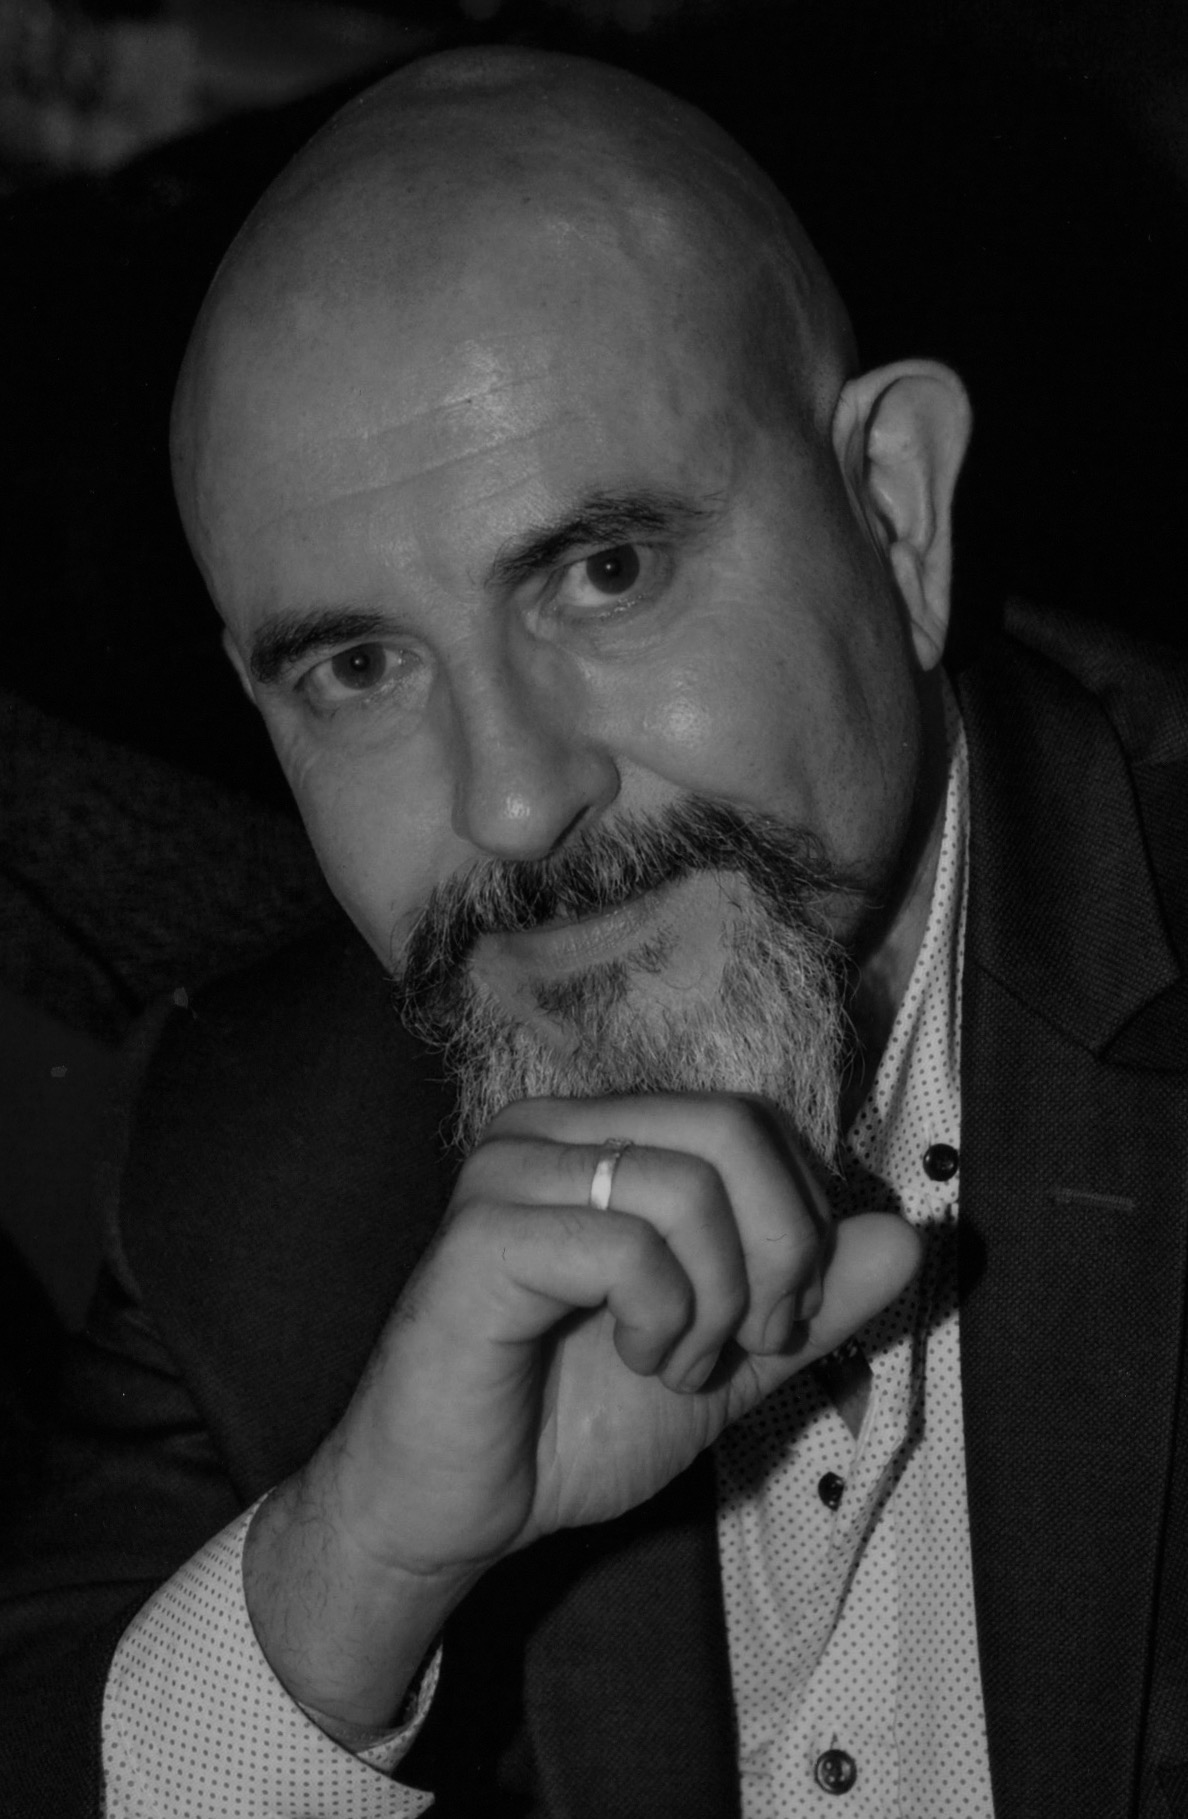
\includegraphics[width=3cm]{\upath/Pictures/authorphoto.jpg}}; 

% ------EAN--------------------------------------------------------------------------------------
\node at (current page.north west)   [xshift= 15cm,  yshift=-24cm, anchor=north west]  {
\includegraphics[width=4cm]{\upath/template.inc/BookModel/BookPictures/ean-white.pdf} }; 

% ------TITRE DE BAS DE PAGE --------------------------------------------------------------------------------------
\node at (current page.center)  [xshift=0cm, yshift=-11cm, text opacity=1]  { {\centering \color{white}\bfseries\sffamily \ubooktitleMain} } ; 

\end{tikzpicture} 
\vfill
\endgroup

  

\end{document}
